\documentclass[fleqn, a4paper, twoside]{article} 


%%%%%%% UNKNOWN %%%%%%%%%%%%%%%%%%%%%%%%%%%%%%%%%%%%%%%%%%%%%%%%%%%%%%%%%%%%%%%
\usepackage{float}
\newcommand{\0}{\langle 0\rangle}

%%%%%%%%%%%%%%%%%%%%%%%%%%%%%%%%%%%%%%%%%%%%%%%%%%%%%%%%%%%%%%%%%%%%%%%%%%%%%%%

%%%%%%%% Measures for printing. %%%%%%%%%%%%%%%%%%%%%%%%%%%%%%%%%%%%%%%%%%%%%%%
\usepackage[
	top = 1.15 in, 
	bottom = 1.25 in,
	left = 1.15 in, 
	right = 1.15 in,
	includehead]{geometry}
% font sizes
\usepackage{scrextend}
\changefontsizes{12pt}
%%%%%%%%%%%%%%%%%%%%%%%%%%%%%%%%%%%%%%%%%%%%%%%%%%%%%%%%%%%%%%%%%%%%%%%%%%%%%%%

%%%%%%%%% Measures for online reading. %%%%%%%%%%%%%%%%%%%%%%%%%%%%%%%%%%%%%%%%
%\usepackage[
%	top = 1.15 cm, 
%	bottom = 2.25 cm,
%	left = 1.15 cm, 
%	right =1.15 cm,
%	includehead]{geometry}
% font sizes
%\usepackage{scrextend}
%\changefontsizes{14pt}
%%%%%%%%%%%%%%%%%%%%%%%%%%%%%%%%%%%%%%%%%%%%%%%%%%%%%%%%%%%%%%%%%%%%%%%%%%%%%%%

%%%%%%%%% Other printing measures. %%%%%%%%%%%%%%%%%%%%%%%%%%%%%%%%%%%%%%%%%%%%
\setlength\parskip{3 pt}
\setlength\parindent{0 em}
\raggedbottom % Bottom is not strict.
%%%%%%%%%%%%%%%%%%%%%%%%%%%%%%%%%%%%%%%%%%%%%%%%%%%%%%%%%%%%%%%%%%%%%%%%%%%%%%%

%%%%%%%%%% Font selection and packages. %%%%%%%%%%%%%%%%%%%%%%%%%%%%%%%%%%%%%%%
\usepackage[utf8x]{inputenc}
\usepackage{mathptmx}
\usepackage[T1]{fontenc}
\usepackage{amsfonts,amssymb,amsmath,amsrefs}
\usepackage{microtype}
\usepackage[all]{nowidow}
\usepackage{changepage}
%%%%%%%%%%%%%%%%%%%%%%%%%%%%%%%%%%%%%%%%%%%%%%%%%%%%%%%%%%%%%%%%%%%%%%%%%%%%%%%

%%%%%%%%%%%%%%%% Other packages. %%%%%%%%%%%%%%%%%%%%%%%%%%%%%%%%%%%%%%%%%%%%%%
\usepackage[british]{babel}
\usepackage{amscd, amssymb, amsmath, amsrefs} % AMS Packages
\usepackage{makeidx}	% Make index
\usepackage{multicol}	% Several columns of text
\usepackage{booktabs}	% Publishing-quality tables
\usepackage{cancel}		% Draw diagonal lines (“cancelling” a term) 
\usepackage{sidecap}	% Side captions
\usepackage{exsheets}	% Package for exercises
\SetupExSheets{headings = runin}
\usepackage{wrapfig}	% Wrapping text around figures
\usepackage{stmaryrd}	% Double brackets
\usepackage{setspace}	% Line spacing
\spacing{1.15}
\usepackage{stackrel}
\usepackage{etoolbox}
\usepackage[bb=ams, cal=euler, scr=rsfso , frak=euler]{mathalpha}
\usepackage{caption}
\usepackage{mathdots, mathtools} 
\usepackage{subfigure}
\usepackage{array}
\usepackage{polynom}
\usepackage[pdf,all]{xy} 
\xyoption{line}
\CompileMatrices
%%%%%%%%%%%%%%%%%%%%%%%%%%%%%%%%%%%%%%%%%%%%%%%%%%%%%%%%%%%%%%%%%%%%%%%%%%%%%%%

%%%%%%%%%%%%%%%%%%%%%%%%%%% TikZ SETUP %%%%%%%%%%%%%%%%%%%%%%%%%%%%%%%%%%%%%%%%
\usepackage{pgf,tikz}
\usepackage{tikz-cd}
\pgfdeclarelayer{bg}    % Declaro background layer.
\pgfsetlayers{bg, main}  % Order layers.
\usetikzlibrary{calc}
\usetikzlibrary{matrix, arrows}
\usetikzlibrary{trees}

%%%%%%%%%%%%%% Tree macros %%%%%%%%%%%%%%%%
%%%%%%%%%%%%%% Edge and vertex styles %%%%%
\tikzset{%
    inner/.style={%
    	circle,draw=black, fill=pagecolor, inner sep=1pt,minimum size=5pt
    	},
    leaf/.style={%
    circle, draw=pagecolor, fill=pagecolor, inner sep=3 pt,minimum size=5 pt
    },
}

\newcommand{\fork}[7]{
\begin{tikzpicture}[scale = .75]
	\begin{pgfonlayer}{main}
		\node [style=inner] (0) at (0, 0) {$#3$};
		\node [style=inner] (2) at (-1, 1) {$#1$};
		\node [style=inner] (9) at (1, 1) {$#2$};
		\node [style=leaf] (10) at (0, -1.25) {};
		\node [style=leaf] (11) at (-1.5, 2) {$#4$};
		\node [style=leaf] (12) at (-0.5, 2) {$#5$};
		\node [style=leaf] (13) at (0.5, 2) {$#6$};
		\node [style=leaf] (14) at (1.5, 2) {$#7$};
	\end{pgfonlayer}
	\begin{pgfonlayer}{bg}
		\draw (2.center) to (0.center);
		\draw (0.center) to (9.center);
		\draw (0.center) to (10.center);
		\draw (2.center) to (11.center);
		\draw (12.center) to (2.center);
		\draw (13.center) to (9.center);
		\draw (9.center) to (14.center);
	\end{pgfonlayer}
\end{tikzpicture}}

\newcommand{\smallfork}[7]{
\begin{tikzpicture}[scale = .50]
	\begin{pgfonlayer}{main}
		\node [style=inner] (0) at (0, 0) {$#3$};
		\node [style=inner] (2) at (-1, 1) {$#1$};
		\node [style=inner] (9) at (1, 1) {$#2$};
		\node [style=leaf] (10) at (0, -1.25) {};
		\node [style=leaf,anchor = south east] (11) at (-1.5, 2) {$#4$};
		\node [style=leaf,anchor = south] (12) at (-0.5, 2) {$#5$};
		\node [style=leaf, anchor = south] (13) at (0.5, 2) {$#6$};
		\node [style=leaf, anchor = south west] (14) at (1.5, 2) {$#7$};
	\end{pgfonlayer}
	\begin{pgfonlayer}{bg}
		\draw (2.center) to (0.center);
		\draw (0.center) to (9.center);
		\draw (0.center) to (10.center);
		\draw (2.center) to (11.center);
		\draw (12.center) to (2.center);
		\draw (13.center) to (9.center);
		\draw (9.center) to (14.center);
	\end{pgfonlayer}
\end{tikzpicture}}


\newcommand{\leftc}[5]{
	\begin{tikzpicture}[scale = .75]
\begin{pgfonlayer}{main}
		\node[style = inner] (0) at (-1, 1) {$#1$};
		\node[style = inner] (1) at (0, 0) {$#2$};
		\node[style = leaf] (2) at (1, 1) {$#5$};
		\node[style = leaf] (3) at (0, 2) {$#4$};
		\node[style = leaf] (4) at (-2, 2) {$#3$};
		\node (5) at (0, -1) {};
		\end{pgfonlayer}
	\begin{pgfonlayer}{bg}
		\draw (1) to (0);
		\draw (2.center) to (1);
		\draw (3.center) to (0);
		\draw (4.center) to (0);
		\draw (5.center) to (1);
		\end{pgfonlayer}	
\end{tikzpicture}
}


\newcommand{\smallb}[3]{
	\begin{tikzpicture}[scale = .50]
\begin{pgfonlayer}{main}
		\node[style = leaf] (0) at (-1, 1) {$#2$};
		\node[style = inner] (1) at (0, 0) {$#1$};
		\node[style = leaf] (2) at (1, 1) {$#3$};
		\node (5) at (0, -1) {};
		\end{pgfonlayer}
	\begin{pgfonlayer}{bg}
		\draw (1) to (0);
		\draw (2.center) to (1);
		\draw (5.center) to (1);
		\end{pgfonlayer}	
\end{tikzpicture}
}
\newcommand{\hplus}{\mathsymbol{.5}{+}}
\newcommand{\hotimes}{\mathsymbol{.5}{\otimes}}

\newcommand{\Tw}{\mathsf{Tw}}
\newcommand{\stick}[1]{
	\begin{tikzpicture}[scale = .50]
\begin{pgfonlayer}{main}
		\node[style = leaf] (0) at (0, 2) {$#1$};
		\node[style = leaf] (1) at (0, 0) {};
		\end{pgfonlayer}
	\begin{pgfonlayer}{bg}
		\draw (1) to (0);
		\end{pgfonlayer}	
\end{tikzpicture}
}

\newcommand{\smallleftc}[5]{
	\begin{tikzpicture}[scale = .50]
\begin{pgfonlayer}{main}
		\node[style = inner] (0) at (-1, 1) {$#1$};
		\node[style = inner] (1) at (0, 0) {$#2$};
		\node[style = leaf] (2) at (1, 1) {$#5$};
		\node[style = leaf] (3) at (0, 2) {$#4$};
		\node[style = leaf] (4) at (-2, 2) {$#3$};
		\node (5) at (0, -1) {};
		\end{pgfonlayer}
	\begin{pgfonlayer}{bg}
		\draw (1) to (0);
		\draw (2.center) to (1);
		\draw (3.center) to (0);
		\draw (4.center) to (0);
		\draw (5.center) to (1);
		\end{pgfonlayer}	
\end{tikzpicture}
}

\newcommand{\inlineleftc}[5]{
	\begin{tikzpicture}[scale = .50, baseline= -10 mm]
\begin{pgfonlayer}{main}
		\node[style = inner] (0) at (-1, 1) {$#1$};
		\node[style = inner] (1) at (0, 0) {$#2$};
		\node[style = leaf] (2) at (1, 1) {$#5$};
		\node[style = leaf] (3) at (0, 2) {$#4$};
		\node[style = leaf] (4) at (-2, 2) {$#3$};
		\node (5) at (0, -1) {};
		\end{pgfonlayer}
	\begin{pgfonlayer}{bg}
		\draw (1) to (0);
		\draw (2.center) to (1);
		\draw (3.center) to (0);
		\draw (4.center) to (0);
		\draw (5.center) to (1);
		\end{pgfonlayer}	
\end{tikzpicture}
}

\newcommand{\Leftc}[7]{
	\begin{tikzpicture}[scale = .75]
\begin{pgfonlayer}{main}
		\node[style = inner] (0) at (-1, 1) {$#2$};
		\node[style = inner] (1) at (0, 0) {$#1$};
		\node[style = leaf] (2) at (1, 1) {$#7$};
		\node[style = leaf] (3) at (0, 2) {$#6$};
		\node[style = inner] (4) at (-2, 2) {$#3$};
		\node[style = leaf] (5) at (-3, 3) {$#4$};
		\node[style = leaf] (6) at (-1, 3) {$#5$};
		\node (7) at (0, -1) {}; %theRoot
		\end{pgfonlayer}
	\begin{pgfonlayer}{bg}
		\draw (1) to (0);
		\draw (2.center) to (1);
		\draw (3.center) to (0);
		\draw (4.center) to (0);
		\draw (7.center) to (1);
		\draw (4.center) to (6);
		\draw (4.center) to (5);
		\end{pgfonlayer}	
\end{tikzpicture}
}

\newcommand{\smallLeftc}[7]{
	\begin{tikzpicture}[scale = .50]
\begin{pgfonlayer}{main}
		\node[style = inner] (0) at (-1, 1) {$#2$};
		\node[style = inner] (1) at (0, 0) {$#1$};
		\node[style = leaf] (2) at (1, 1) {$#7$};
		\node[style = leaf] (3) at (0, 2) {$#6$};
		\node[style = inner] (4) at (-2, 2) {$#3$};
		\node[style = leaf] (5) at (-3, 3) {$#4$};
		\node[style = leaf] (6) at (-1, 3) {$#5$};
		\node (7) at (0, -1) {}; %theRoot
		\end{pgfonlayer}
	\begin{pgfonlayer}{bg}
		\draw (1) to (0);
		\draw (2.center) to (1);
		\draw (3.center) to (0);
		\draw (4.center) to (0);
		\draw (7.center) to (1);
		\draw (4.center) to (6);
		\draw (4.center) to (5);
		\end{pgfonlayer}	
\end{tikzpicture}
}

\newcommand{\Rightc}[7]{
	\begin{tikzpicture}[scale = .75]
\begin{pgfonlayer}{main}
		\node[style = inner] (0) at (1, 1) {$#2$};
		\node[style = inner] (1) at (0, 0) {$#1$};
		\node[style = leaf] (2) at (-1, 1) {$#4$};
		\node[style = leaf] (3) at (0, 2) {$#5$};
		\node[style = inner] (4) at (2, 2) {$#3$};
		\node[style = leaf] (5) at (3, 3) {$#7$};
		\node[style = leaf] (6) at (1, 3) {$#6$};
		\node (7) at (0, -1) {}; %theRoot
		\end{pgfonlayer}
	\begin{pgfonlayer}{bg}
		\draw (1) to (0);
		\draw (2.center) to (1);
		\draw (3.center) to (0);
		\draw (4.center) to (0);
		\draw (7.center) to (1);
		\draw (4.center) to (6);
		\draw (4.center) to (5);
		\end{pgfonlayer}	
\end{tikzpicture}
}


\newcommand{\smallRightc}[7]{
	\begin{tikzpicture}[scale = .50]
\begin{pgfonlayer}{main}
		\node[style = inner] (0) at (1, 1) {$#2$};
		\node[style = inner] (1) at (0, 0) {$#1$};
		\node[style = leaf] (2) at (-1, 1) {$#4$};
		\node[style = leaf] (3) at (0, 2) {$#5$};
		\node[style = inner] (4) at (2, 2) {$#3$};
		\node[style = leaf] (5) at (3, 3) {$#7$};
		\node[style = leaf] (6) at (1, 3) {$#6$};
		\node (7) at (0, -1) {}; %theRoot
		\end{pgfonlayer}
	\begin{pgfonlayer}{bg}
		\draw (1) to (0);
		\draw (2.center) to (1);
		\draw (3.center) to (0);
		\draw (4.center) to (0);
		\draw (7.center) to (1);
		\draw (4.center) to (6);
		\draw (4.center) to (5);
		\end{pgfonlayer}	
\end{tikzpicture}
}

\newcommand{\Leftr}[7]{
	\begin{tikzpicture}[scale = .75]
\begin{pgfonlayer}{main}
		\node[style = inner] (0) at (-1, 1) {$#2$};
		\node[style = inner] (1) at (0, 0) {$#1$};
		\node[style = leaf] (2) at (1, 1) {$#7$};
		\node[style = inner] (3) at (0, 2) {$#3$};
		\node[style = leaf] (4) at (-2, 2) {$#6$};
		\node[style = leaf] (5) at (-1, 3) {$#4$};
		\node[style = leaf] (6) at (1, 3) {$#5$};
		\node (7) at (0, -1) {}; %theRoot
		\end{pgfonlayer}
	\begin{pgfonlayer}{bg}
		\draw (1) to (0);
		\draw (2.center) to (1);
		\draw (3.center) to (0);
		\draw (4.center) to (0);
		\draw (7.center) to (1);
		\draw (3.center) to (6);
		\draw (3.center) to (5);
		\end{pgfonlayer}	
\end{tikzpicture}
}


\newcommand{\smallLeftr}[7]{
	\begin{tikzpicture}[scale = .50]
\begin{pgfonlayer}{main}
		\node[style = inner] (0) at (-1, 1) {$#2$};
		\node[style = inner] (1) at (0, 0) {$#1$};
		\node[style = leaf] (2) at (1, 1) {$#7$};
		\node[style = inner] (3) at (0, 2) {$#3$};
		\node[style = leaf] (4) at (-2, 2) {$#6$};
		\node[style = leaf] (5) at (-1, 3) {$#4$};
		\node[style = leaf] (6) at (1, 3) {$#5$};
		\node (7) at (0, -1) {}; %theRoot
		\end{pgfonlayer}
	\begin{pgfonlayer}{bg}
		\draw (1) to (0);
		\draw (2.center) to (1);
		\draw (3.center) to (0);
		\draw (4.center) to (0);
		\draw (7.center) to (1);
		\draw (3.center) to (6);
		\draw (3.center) to (5);
		\end{pgfonlayer}	
\end{tikzpicture}
}
\newcommand{\Rightl}[7]{
	\begin{tikzpicture}[scale = .75]
\begin{pgfonlayer}{main}
		\node[style = leaf] (0) at (-1, 1) {$#4$};
		\node[style = inner] (1) at (0, 0) {$#1$};
		\node[style = inner] (2) at (1, 1) {$#2$};
		\node[style = inner] (3) at (0, 2) {$#3$};
		\node[style = leaf] (4) at (2, 2) {$#7$};
		\node[style = leaf] (5) at (-1, 3) {$#5$};
		\node[style = leaf] (6) at (1, 3) {$#6$};
		\node (7) at (0, -1) {}; %theRoot
		\end{pgfonlayer}
	\begin{pgfonlayer}{bg}
		\draw (1) to (0);
		\draw (2.center) to (1);
		\draw (3.center) to (2);
		\draw (4.center) to (2);
		\draw (7.center) to (1);
		\draw (3.center) to (6);
		\draw (3.center) to (5);
		\end{pgfonlayer}	
\end{tikzpicture}
}

\newcommand{\smallRightl}[7]{
	\begin{tikzpicture}[scale = .50]
\begin{pgfonlayer}{main}
		\node[style = leaf] (0) at (-1, 1) {$#4$};
		\node[style = inner] (1) at (0, 0) {$#1$};
		\node[style = inner] (2) at (1, 1) {$#2$};
		\node[style = inner] (3) at (0, 2) {$#3$};
		\node[style = leaf] (4) at (2, 2) {$#7$};
		\node[style = leaf] (5) at (-1, 3) {$#5$};
		\node[style = leaf] (6) at (1, 3) {$#6$};
		\node (7) at (0, -1) {}; %theRoot
		\end{pgfonlayer}
	\begin{pgfonlayer}{bg}
		\draw (1) to (0);
		\draw (2.center) to (1);
		\draw (3.center) to (2);
		\draw (4.center) to (2);
		\draw (7.center) to (1);
		\draw (3.center) to (6);
		\draw (3.center) to (5);
		\end{pgfonlayer}	
\end{tikzpicture}
}

\newcommand{\rightc}[5]{
\begin{tikzpicture}[scale = .75]
\begin{pgfonlayer}{main}
		\node[style = leaf] (0) at (-1, 1) {$#3$};
		\node[style = inner] (1) at (0, 0) {$#1$};
		\node[style = inner] (2) at (1, 1) {$#2$};
		\node[style = leaf] (3) at (0, 2) {$#4$};
		\node[style = leaf] (4) at (2, 2) {$#5$};
		\node (5) at (0, -1) {};
		\end{pgfonlayer}
	\begin{pgfonlayer}{bg}
		\draw (1) to (0);
		\draw (2.center) to (1);
		\draw (3.center) to (2);
		\draw (4.center) to (2);
		\draw (5.center) to (1);
		\end{pgfonlayer}	
\end{tikzpicture}
}

\newcommand{\smallrightc}[5]{
\begin{tikzpicture}[scale = .5]
\begin{pgfonlayer}{main}
		\node[style = leaf] (0) at (-1, 1) {$#3$};
		\node[style = inner] (1) at (0, 0) {$#1$};
		\node[style = inner] (2) at (1, 1) {$#2$};
		\node[style = leaf] (3) at (0, 2) {$#4$};
		\node[style = leaf] (4) at (2, 2) {$#5$};
		\node (5) at (0, -1) {};
		\end{pgfonlayer}
	\begin{pgfonlayer}{bg}
		\draw (1) to (0);
		\draw (2.center) to (1);
		\draw (3.center) to (2);
		\draw (4.center) to (2);
		\draw (5.center) to (1);
		\end{pgfonlayer}	
\end{tikzpicture}
}
\newcommand{\mathsymbol}[2]{
	\begin{tikzpicture}
        \node at(0,0){};
        \node at(0,#1){$#2$};
    \end{tikzpicture}
} % TIKZ MACROS TO DRAW TREES 
\tikzcdset{arrow style=tikz, diagrams={>=stealth}}
%%%%%%%%%%%%%%%%%%%%%%%%%%%%%%%%%%%%%%%%%%%%%%%%%%%%%%%%%%%%%%%%%%%%%%%%%%%%%%%

%%%%%%%%%%%%% Colours throughout document %%%%%%%%%%%%%%%%%%%%%%%%%%%%%%%%%%%%%
\usepackage{xcolor}
\definecolor{trinityblue}{rgb}{0.05, 0.45,0.75}
\definecolor{trinitygray}{rgb}{0.33, 0.34,0.35}
\definecolor{mpg-gruen}{rgb}{0.00, 0.428,0.404}
\definecolor{pagecolor}{rgb}{1, 1, 0.88}
%%%%%%%%%%%%%%%%%%%%%%%%%%%%%%%%%%%%%%%%%%%%%%%%%%%%%%%%%%%%%%%%%%%%%%%%%%%%%%%

%%%%%%%%% Getting LaTeX to use letter Sha %%%%%%%%%%%%%%%%%%%%%%%%%%%%%%%%%%%%%
\DeclareFontFamily{U}{wncy}{}
\DeclareFontShape{U}{wncy}{m}{n}{<->wncyr10}{}
\DeclareSymbolFont{mcy}{U}{wncy}{m}{n}
\DeclareMathSymbol{\ShaL}{\mathord}{mcy}{"58} 
\usepackage{scalerel}[2016/12/29]
\newcommand{\Sha}{{\scaleobj{0.75}{\ShaL}}}
%%%%%%%%%%%%%%%%%%%%%%%%%%%%%%%%%%%%%%%%%%%%%%%%%%%%%%%%%%%%%%%%%%%%%%%%%%%%%%%
 
%%%%%%%%%%%%%%% Fancy headers set-up %%%%%%%%%%%%%%%%%%%%%%%%%%%%%%%%%%%%%%%%%%
\usepackage{fancyhdr}

\pagestyle{fancy}
\fancyhead[RE]{\small\it Algebraic operads}
\fancyhead[LO]{\small\it Winter Lecture Series 2021/2022}
\fancyhead[RO,LE]{\small\textbf\thepage}
\renewcommand{\headrulewidth}{0 pt}
\cfoot{}

\fancypagestyle{references}
{\fancyhead[RE]{\small\it References}
\fancyhead[LO]{\small\it References}
\fancyhead[RO,LE]{\small\bf\thepage}
\fancyfoot[L,R,C]{}
\renewcommand{\headrulewidth}{0 pt}}
%%%%%%%%%%%%%%%%%%%%%%%%%%%%%%%%%%%%%%%%%%%%%%%%%%%%%%%%%%%%%%%%%%%%%%%%%%%%%%%





%%%%%%%%%%%%%%%%%% ENUMERATE STUFF %%%%%%%%%%%%%%%%%%%%%%%%%%%%%%%%%%%%%%%%%%%%
\usepackage[shortlabels]{enumitem} 
\setenumerate{label= (\arabic*)}

\newenvironment{tenumerate}{
 \begin{enumerate}
  \setlength{\itemsep}{0pt}
  \setlength{\parskip}{0pt}
}{\end{enumerate}}

\newenvironment{titemize}{
\begin{itemize}
  \setlength{\itemsep}{0pt}
  \setlength{\parskip}{0pt}
}{\end{itemize}}
%%%%%%%%%%%%%%%%%%%%%%%%%%%%%%%%%%%%%%%%%%%%%%%%%%%%%%%%%%%%%%%%%%%%%%%%%%%%%%%


\definecolor{newcol}{rgb}{0,0,0}
\definecolor{deepblue}{rgb}{0.0, 0.28, 0.67}
%{0.5, 0.0, 0.13}
\DeclareTextFontCommand{\new}{\color{black}\em}

%%%%%%%%%%%%%%%% Hyperlinks set up %%%%%%%%%%%%%%%%%%%%%%%%%%%%%%%%%%%%%%%%%%%%
\usepackage[pdftex, 
			colorlinks, 
			bookmarks = true, 
			bookmarksnumbered = true]{hyperref}
\hypersetup{colorlinks, 
			linkcolor={mpg-gruen}, 
			citecolor={mpg-gruen}, 
			urlcolor={mpg-gruen}} 
%%%%%%%%%%%%%%%%%%%%%%%%%%%%%%%%%%%%%%%%%%%%%%%%%%%%%%%%%%%%%%%%%%%%%%%%%%%%%%%

%%%%%%%%%%%%%%%%% Brackets are equations %%%%%%%%%%%%%%%%%%%%%%%%%%%%%%%%%%%%%%
% let \[ and \] be the same as \begin{equation} and \end{equation}
\makeatletter
\AtBeginDocument{%
  \let\[\@undefined
  
\DeclareRobustCommand{\[}{\begin{equation}}%
  \let\]\@undefined
  
\DeclareRobustCommand{\]}{\end{equation}}%
}
\makeatother 
% but only print equation numbers if needed
\mathtoolsset{showonlyrefs,showmanualtags}
%%%%%%%%%%%%%%%%%%%%%%%%%%%%%%%%%%%%%%%%%%%%%%%%%%%%%%%%%%%%%%%%%%%%%%%%%%%%%%%

%%%%%%%%%%%%% Theorem styles set-up %%%%%%%%%%%%%%%%%%%%%%%%%%%%%%%%%%%%%%%%%%%
\usepackage{amsthm}
\usepackage{thmtools}
\newtheoremstyle{mytheorem}
  {\topsep}   % ABOVESPACE
  {\topsep}   % BELOWSPACE
  {\itshape}  % BODYFONT
  {0pt}       % INDENT (empty value is the same as 0pt)
  {\bfseries\color{newcol}} % HEADFONT
  {\color{newcol}}         % HEADPUNCT
  {5pt plus 1pt minus 1pt} % HEADSPACE
  {}          % CUSTOM-HEAD-SPEC
  
\theoremstyle{mytheorem}
\newtheorem{theorem}{Theorem}[section]
\newtheorem{proposition}[theorem]{Proposition}
\newtheorem{corollary}[theorem]{Corollary}
\newtheorem{lemma}[theorem]{Lemma}
\newtheorem*{conj*}{Conjecture}
%\newtheorem{question}[theorem]{Question}

 \newtheoremstyle{introthm}
  {\topsep}   % ABOVESPACE
  {\topsep}   % BELOWSPACE
  {\itshape}  % BODYFONT
  {0pt}       % INDENT (empty value is the same as 0pt)
  {\bfseries\color{newcol}} % HEADFONT
  {\color{newcol}{.}}         % HEADPUNCT
  {5pt plus 1pt minus 1pt} % HEADSPACE
  {}          % CUSTOM-HEAD-SPEC
 
  
\theoremstyle{introthm}
\newtheorem{introthm}{Theorem}
\newtheorem*{introcor}{Corollary}
\renewcommand{\theintrothm}{\Alph{introthm}}
 % Para teoremas en la introducción


\newtheoremstyle{mydefinition}
{\topsep}   % ABOVESPACE
{\topsep}   % BELOWSPACE
{}  % BODYFONT
{0pt}       % INDENT (empty value is the same as 0pt)
{\bfseries\color{newcol}} % HEADFONT
{\color{newcol}}         % HEADPUNCT
{5pt plus 1pt minus 1pt} % HEADSPACE
{}          % CUSTOM-HEAD-SPEC

\theoremstyle{mydefinition}
\newtheorem{definition}[theorem]{Definition}
\newtheorem{obs}[theorem]{Observation}
\newtheorem{rmk}[theorem]{Remark}
\newtheorem{problem}[theorem]{Problem}
\newtheorem{example}[theorem]{Example}
\newtheorem{note}[theorem]{Note}
\newtheorem{variante}[theorem]{Variant}

\newtheoremstyle{mydefinition2}
{\topsep}   % ABOVESPACE
{\topsep}   % BELOWSPACE
{}  % BODYFONT
{0pt}       % INDENT (empty value is the same as 0pt)
{\bfseries\color{newcol}} % HEADFONT
{\color{newcol}{.}}         % HEADPUNCT
{5pt plus 1pt minus 1pt} % HEADSPACE
{}          % CUSTOM-HEAD-SPEC

\theoremstyle{mydefinition2}
\newtheorem*{definition*}{Definition}
\newtheorem*{remark*}{Remark}
\newtheorem*{obs*}{Observation}
\newtheorem*{example*}{Example}

% For specifying a named theorem
\theoremstyle{plain} % just in case the style had changed
\newcommand{\thistheoremname}{}
\newtheorem{genericthm}[theorem]{\thistheoremname}
\newenvironment{namedthm}[1]
{\renewcommand{\thistheoremname}{#1}%
 \begin{genericthm}}
{\end{genericthm}}

\theoremstyle{mytheorem}
\newtheorem*{theorem*}{Theorem}
\newtheorem*{question*}{Question}
%%%%%%%%%%%%%%%%%%%%%%%%%%%%%%%%%%%%%%%%%%%%%%%%%%%%%%%%%%%%%%%%%%%%%%%%%%%%%%%

%%%%%%%% AUTHOR INFORMATION %%%%%%%%%%%%%%%%%%%%%%%%%%%%%%%%%%%%%%%%%%%%%%%%%%%
\newcommand{\myauthor}[3]{
\noindent
\begin{minipage}[t]{.45\textwidth}
\begin{flushright}
\textsc{#1} \\
{\footnotesize\texttt{#2}}
\end{flushright} 
\end{minipage}
\qquad
\begin{minipage}[t]{.45\textwidth}
#3
\end{minipage}
}
%%%%%%%%%%%%%%%%%%%%%%%%%%%%%%%%%%%%%%%%%%%%%%%%%%%%%%%%%%%%%%%%%%%%%%%%%%%%%%%
 
%%%%%%%%%%%%%%%%%%%%%% TODO NOTES SET-UP %%%%%%%%%%%%%%%%%%%%%%%%%%%%%%%%%%%%%%
\usepackage{xargs}                      
\usepackage[colorinlistoftodos,prependcaption,textsize=small]{todonotes}
\newcommand{\hacer}[1]{
	\todo[
		inline,
		linecolor= mpg-gruen,
		backgroundcolor=mpg-gruen!25!white,
		bordercolor=mpg-gruen]
		{#1}
		}
\newcommandx{\unsure}[2][1=]{
	\todo[
		linecolor=blue,
		backgroundcolor=blue!25!white,
		bordercolor=blue,#1
	]
	{#2}
	}
\newcommandx{\change}[2][1=]{
	\todo[
		linecolor=blue,
		backgroundcolor=blue!25,
		bordercolor=blue,
		#1]
		{#2}
		}
\definecolor{col1}{rgb}{0.8, 0.8, 1.0}
\definecolor{col2}{rgb}{0.9, 0.9, 0.98}
\definecolor{col3}{rgb}{0.71, 0.49, 0.86}
%%%%%%%%%%%%%%%%%%%%%%%%%%%%%%%%%%%%%%%%%%%%%%%%%%%%%%%%%%%%%%%%%%%%%%%%%%%%%%%

%%%%%%%%%%%%%%%%%%%%%% To write pseudo-code %%%%%%%%%%%%%%%%%%%%%%%%%%%%%%%%%%%
\usepackage{algorithm}
\usepackage[noend]{algpseudocode}
\makeatletter
\def\BState{\State\hskip-\ALG@thistlm}
\makeatother
%%%%%%%%%%%%%%%%%%%%%%%%%%%%%%%%%%%%%%%%%%%%%%%%%%%%%%%%%%%%%%%%%%%%%%%%%%%%%%%

%%%%%%%%% MATH MACROS %%%%%%%%%%%%%%%%%%%%%%%%%%%%%%%%%%%%%%%%%%%%%%%%%%%%%%%%%

\mathchardef\hy="2D % Define a "math hyphen"
\newcommand{\antishriek}{\text{\raisebox{\depth}{\textexclamdown}}}
\newcommand{\eantishriek}{\emph{\text{\raisebox{\depth}{\textexclamdown}}}}

%%%%%%%%%%% CATEGORIES ETC %%%%%%%%%%%
\newcommand{\GSet}{\mathsf{Fin}^\times}
\newcommand{\FSet}{\mathsf{Fin}}
\newcommand{\Fun}{\mathsf{Fun}}
\newcommand{\Set}{\mathsf{Set}}
\newcommand{\DCSH}{\mathsf{DCSH}}
\newcommand{\kMod}{{}_\kk\mathsf{Mod}}
\newcommand{\kmod}{{}_\kk\mathsf{mod}}
\newcommand{\kCh}{{}_\kk\mathsf{Ch}}
\newcommand{\Sp}{\mathsf{Sp}}
\newcommand{\kSp}{{}_\kk\mathsf{Sp}}
\newcommand{\GVec}{\mathsf{Vec}_q^\times}
\newcommand{\Opr}{\mathsf{Opr}}
\newcommand{\NS}{\mathsf{NS}}
\newcommand{\SC}{SC}
\newcommand{\Mod}{\mathsf{Mod}}
\newcommand{\Gmod}{\mathsf{GMod}}
\newcommand{\nsMod}{{}_{\mathrm{ns}}\mathsf{Mod}}
\newcommand{\aut}{\operatorname{aut}}
\newcommand{\SMod}{{}_\Sigma\mathsf{Mod}}
\newcommand{\dgSMod}{{}_\Sigma\mathsf{dgMod}}
\newcommand{\gSMod}{{}_\Sigma\mathsf{gMod}}
\newcommand{\coker}{\operatorname{coker}}
\newcommand{\Ho}{\operatorname{Ho}}
\newcommand{\DC}{\mathsf{DC}}
\newcommand{\DA}{\mathsf{DA}}

\renewcommand{\tt}{\otimes}
\newcommand{\vv}{\vert}
\newcommand{\imor}{\interleave\kern-.45em\longrightarrow}
\newcommand{\ps}{\mathbin\parallel}

\newcommand\category[1]{\mathsf{#1}}
\newcommand\spe[1]{\mathcal{#1}}
\newcommand\id{\mathrm{id}}
\newcommand\place{\mathord-}

\DeclarePairedDelimiter\abs{\lvert}{\rvert}


\definecolor{sqsqsq}{rgb}{0.13,0.13,0.13}
\definecolor{aqaqaq}{rgb}{0.63,0.63,0.63}




\newcommand{\dd}{\partial}
\newcommand{\?}{\,?\,}
\renewcommand{\k}{[k]}
\newcommand{\n}{[n]}
\newcommand{\kk}{\Bbbk}

\newcommand\inter[1]{\llbracket#1\rrbracket}

%%%%%%%% HOMOLOGICAL ALGEBRA MACROS.
\newcommand{\bt}{\bullet}
\newcommand{\Aut}{\operatorname{Aut}}
\newcommand{\Ext}{\operatorname{Ext}}
\newcommand{\Tor}{\operatorname{Tor}}
\newcommand{\PAlg}{\mathsf{Alg}_{\geqslant 0}}
\newcommand{\Cog}{\mathsf{Cog}}
\newcommand{\Alg}{\mathsf{Alg}}
\newcommand{\Cxs}{\mathsf{Ch}_\kk}
\newcommand{\Der}{\operatorname{Der}}
\newcommand{\HH}{\mathrm{HH}}

%%%%%%%%%% NAMED OPERADS %%%%%%%%%
\newcommand{\As}{\mathsf{As}}
\newcommand{\Com}{\mathsf{Com}}
\newcommand{\Lie}{\mathsf{Lie}}

\newcommand{\Q}{\mathbb Q}
\newcommand{\Z}{\mathbb Z}
\newcommand{\NN}{\mathbb N}
\newcommand{\PP}{\mathcal P}
\newcommand{\OO}{\mathcal O}
\newcommand{\MM}{\mathcal M}
\newcommand{\E}{\mathcal{E}}
\newcommand{\CC}{\mathcal{C}}


\newcommand{\hoq}{\!\sslash\!\!}
\newcommand{\adjoint}{\;\substack{\longrightarrow \\[-0.6ex] \longleftarrow}\;}


%%%%% COMMANDS FOR GROEBNER THEORY %%%%%
\newcommand{\lead}[1]{\operatorname{LT}(#1)}
\newcommand{\leadm}[1]{\operatorname{LM}(#1)}
\newcommand{\repl}[3]{\square_{#1}^{#2}(#3)}
\newcommand{\leadc}[1]{\operatorname{LC}(#1)}


\newcommand{\XX}{\mathcal{X}}
\renewcommand{\AA}{\mathcal{A}}
\newcommand{\YY}{\mathcal{Y}}
\newcommand{\End}{\operatorname{End}}
\newcommand{\RR}{\mathcal{R}}
\newcommand{\II}{\mathcal{I}}
\newcommand{\QQ}{\mathcal{Q}}
\newcommand{\FF}{\mathcal{F}}
\newcommand{\GG}{\mathcal G}
\newcommand{\B}[1]{\mathsf{B}(#1)}
\newcommand{\syz}[1]{\mathsf{s}(#1)}

\newcommand{\f}{\mathsf{f}}
\newcommand{\ari}{\operatorname{ar}}
\newcommand{\cone}{\operatorname{cone}}
\newcommand{\hem}{\hspace{0.5 em}} 

 \newcommand{\stt}{\mathbin{\text{\tikz 
[x=1ex,y=1ex,line width=.1ex,line 
join=round] \draw (0,0) rectangle (1,1) 
(1,1) -- (0,0)  (1,0) -- (0,1);}}}


\newcommand{\ind}{\operatorname{Ind}_\PP}

\newcommand{\cof}{\rightarrowtail}
\newcommand{\foc}{\leftarrowtail}
\newcommand{\weq}{\overset{\sim}{\longrightarrow}}
\newcommand{\tcf}{\overset{\sim}{\cof}}
\DeclareMathOperator\sgn{sgn}
\newcommand{\ra}[1]{\renewcommand{\arraystretch}{#1}}

%%%%%%%%%%%%%%%%%%%%%%%%%%%%%%%%%%%%%%%%%%%%%%%%%%%%%%%%%%%%%%%%%%%%%%%%%%%%%%%

%%%%%%%%%%%%%%%%%% Front matter style %%%%%%%%%%%%%%%%%%%%%%%%%%%%%%%%%%%%%%%%%
\renewenvironment{abstract}{%
\small\begin{center}
\begin{minipage}{.9\textwidth}
}
{\par\noindent\end{minipage}\end{center}\vspace{3 em}}
%
\makeatletter
\renewcommand\@maketitle{%
\hfill
\begin{center}\begin{minipage}{0.9 	\textwidth}
\centering
\vskip 6em
\let\footnote\thanks 
{\LARGE \@title \par }
\vspace{1 em}
%\hrulefill
\vskip 1 em
{\large \@author \par}
\vspace{3.5 em}

\end{minipage}\end{center}
\par
}
\makeatother
%
%%%%%%%%%%%%%%%%%%%%%%%%%%%%%%%%%%%%%%%%%%%%%%%%%%%%%%%%%%%%%%%%%%%%%%%%%%%%%%%

%%%%%%%%%%%%%%%%% Textual claims in equations %%%%%%%%%%%%%%%%%%%%%%%%%%%%%%%%%
\newcommand\claim[2][.8]{%
  \begin{minipage}{#1\displaywidth}%
  \itshape
  #2
  \end{minipage}%
}
%%%%%%%%%%%%%%%%%%%%%%%%%%%%%%%%%%%%%%%%%%%%%%%%%%%%%%%%%%%%%%%%%%%%%%%%%%%%%%%

%%%%%%%%%%%%%%%%%% Add blank pages after %%%%%%%%%%%%%%%%%%%%%%%%%%%%%%%%%%%%%%
\usepackage{afterpage}
\newcommand\blankpage{%
    \null
    \thispagestyle{empty}%
    %\addtocounter{page}{-1}%
    \newpage}
%%%%%%%%%%%%%%%%%%%%%%%%%%%%%%%%%%%%%%%%%%%%%%%%%%%%%%%%%%%%%%%%%%%%%%%%%%%%%%%

%%%%%%%%%%%%%%% Set-up the Table of Contents. %%%%%%%%%%%%%%%%%%%%%%%%%%%%%%%%%
\usepackage{titletoc}
\setcounter{section}{-1}
\patchcmd{\section}{\normalfont}{\normalfont\large}{}{}

\titlecontents{chapter}
[0.2em] %
{\bigskip}
%{\contentslabel[\thecontentslabel.]{2em}\hspace{0.667em}}%\thecontentslabel
{\makebox[2em][r]{\thecontentslabel.}\hspace{0.333em}}%\thecontentslabel
{\hspace*{-2em}}
{\hfill\contentspage}[\smallskip]

\titlecontents{section}% <section>
[0.2em]% <left>
{\small}% <above-code>
{\thecontentslabel.\hspace{3pt}}%<numbered-entry-format>; you could also 
%use  {\thecontentslabel. } to show the numbers
{}% <numberless-entry-format>
{\enspace\titlerule*[0.5pc]{.}\contentspage}%<filler-page-format>
\titlecontents*{subsection}% <section>
[1em]% <left>
{\footnotesize}% <above-code>
{\thecontentslabel. \hspace{3pt}}% <numbered-entry-format>; you could also 
%use {\thecontentslabel. } to show the numbers
{}% <numberless-entry-format>
{}% <filler-page-format>
[ --- \ ]% <separator>
[]% <end>
\setcounter{tocdepth}{2}% Display up to \subsection in ToC
%%%%%%%%%%%%%%%%%%%%%%%%%%%%%%%%%%%%%%%%%%%%%%%%%%%%%%%%%%%%%%%%%%%%%%%%%%%%%%%

%%%%%%%%%%%%%%% Title and author %%%%%%%%%%%%%%%%%%%%%%%%%%%%%%%%%%%%%%%%%%%%%%
\title{
	\vspace{-5 em}
	\setstretch{0.85}
		{
		\textbf
			{Algebraic operads, 
			Koszul duality and Gr\"obner bases: 
			an introduction}
		}
	}
\author{P. Tamaroff}
%%%%%%%%%%%%%%%%%%%%%%%%%%%%%%%%%%%%%%%%%%%%%%%%%%%%%%%%%%%%%%%%%%%%%%%%%%%%%%%

\makeindex

\begin{document}
\pagecolor{pagecolor}
\maketitle
\thispagestyle{empty}

\begin{abstract}
This lecture series aim to offer a gentle introduction to the theory of algebraic 
operads, starting with the elements of the theory, and progressing slowly towards
more advanced themes, including (inhomogeneous) Koszul duality theory, Gr\"obner 
bases and higher structures. The course will consist of approximately twelve 
lectures, along with extra talks by willing participants, with the goal of 
introducing extra material to the course, and making them more familiar with the 
theory.
\end{abstract}

\vspace{2 cm}

\begin{center}

\includegraphics[scale=.35]{logoMPG.png}
\end{center}

\vfill
\vfill

\texttt{Note! This is a draft. } \hfill	Berlin, \today


\afterpage{\blankpage}
\newpage

%%%%%%%%%%%%%%%%%%%%% AUTHOR COMMENT AND INFORMATION %%%%%%%%%%%%%%%%%%%%%%%%%%
\vspace*{\fill} 

\emph{These notes were written during the Winter Lecture Series for the academic 
term 2021-2022 at the \emph{Max Planck Institut f\"ur Mathematike in den 
Naturwissenschaften}. We acknowledge the excellent working conditions during the 
time the lecture series took place, which in particular allowed to produce these 
lecture notes.}

\bigskip

\begin{small}
	\myauthor{Pedro Tamaroff}{tamarofp@hu-berlin.de}
	{
		\textsc{Institut für Mathematik},	\\ 
		Johann von Neumann-Haus, 			\\
		Humboldt-Universität zu Berlin, 	\\
		Rudower Chaussee 25, 				\\
		12489 Berlin, Deutschland
									}
\end{small} \afterpage{\blankpage}
\vspace*{\fill} 
\newpage
%%%%%%%%%%%%%%%%%%%%%%%%%%%%%%%%%%%%%%%%%%%%%%%%%%%%%%%%%%%%%%%%%%%%%%%%%%%%%%%

%%%%%%%% TOC PAGE %%%%%%%%%%%%%%%%%%%%%%%%%%%%%%%%%%%%%%%%%%%%%%%%%%%%%%%%%%%%%
\thispagestyle{empty}
\tableofcontents
\afterpage{\blankpage}
\newpage
%%%%%%%%%%%%%%%%%%%%%%%%%%%%%%%%%%%%%%%%%%%%%%%%%%%%%%%%%%%%%%%%%%%%%%%%%%%%%%%



\section{Motivation and history}\label{lecture:theintro}
 
\textbf{Goals.} The goal of this lecture is to give a broad picture of the 
history and pre-history of operads, and some current trends, and give a road-map
for the course.  
  
Operads (topological operads, more precisely) originally appeared as tools in 
algebraic topology and homotopy theory, specifically in the study of iterated loop 
spaces (May, 1972 and Boardman and Vogt before). They also appeared as \emph{comp 
algebras} in Gerstenhaber's work on Hochschild cohomology and topologically as 
Stasheff's `associahedra' for his homotopy characterization of loop spaces (both 
in 1963). The theory of operads, in particular topological and algebraic, saw 
itself very much influenced by homological algebra, category theory, algebraic
geometry, rational homotopy theory and mathematical phyisics. Here we list a few 
examples:

\begin{tenumerate}
\item Stasheff~\cite{Stasheff1970,Stasheff1963,Stasheff1963a} and 
Sugawara~\cite{Sugawara55} studied homotopy associative $H$-spaces, Stasheff 
implicitly discovers a topological non-symmetric operad $K$ and a recognition 
principle for infinite deloopings: a connected topological space is an infinite
loop space if and only if it is acted upon by this topological operad $K$. 

\item Boardmann--Vogt~\cite{Boardman1973,bams/1183530111} studied infinite loop 
spaces, built a PROP that provides a version of an $E_\infty$-operad,and obtained
a recognition principle for infinite loop spaces.

\item Kontsevich~\cite{Kontsevich2003} used $L_\infty$-algebras and configuration 
spaces to prove his deformation quantization theorem that every Poisson manifold
admits a deformation quantization.

\item The above is implied by Kontsevich's the formality theorem: the Lie algebra 
of polyvector fields is $L_\infty$-quasi-isomorphic to the Hochschild complex, and 
$f_1 = \mathsf{HKR}$. 

\item Tamarkin~\cite{Tamarkin2003,Hinich2003} approached this result through 
the formality of the little disks operad $D_2$. Proves that the Hochschild 
complex of a polynomial algebra is \emph{intrinsically formal} as a 
Gerstenhaber algebra.

\item Manifold calculus describes the homotopy type of embedding spaces as certain 
derived operadic module maps and to produces their explicit deloopings using 
little disk operads, due to many authors~\cite{Arone2007, Goodwillie1999, Weiss1996, 
Weiss1999}. We point the reader to~\cite{IdrissiPeccot} for a comprehensive
list of references.

\item Koszul duality~\cite{Ginzburg1994} for algebraic operads and cousins allows
to develop a robust homotopy theory of homotopy algebras~\cite{Vallette2020,
Hinich1999}, cohomology theory, deformation theory, Quillen homology, etc. 
Rational homotopy theory~\cite{Quillen1967,Felix2001,Sullivan1977} motivated 
and heralded the development of the homotopy theory of and Koszul duality
theory for algebraic operads.

\item The study of natural operations on the Hochschild complex of an associative
algebra~\cite{Hochschild1945} lead to a manifold of results beginning with the 
proof that there is an action of the little disks operad $D_2$ on it (Deligne's
conjecture), and the ultimate version by Batanin--Markl~\cite{Batanin2014},
who proved that the operad of natural operations on it has the homotopy type 
of $C_*(D_2)$.  

\end{tenumerate}

Operads are modelled by trees: planar or
non-planar, rooted or not, there exists a monad
of trees that defines them. This idea
 in fact extends
to more complicated situations, like that of
properads, dioperads or modular operads,
in the sense that relaxing these
graphs to allow for more structure 
produces other type of algebraic structures
of interest. The following table
gives the reader a ``taxonomy cheat sheet''
for operads and their kin; we will, for better
or worse, defer from diving into the curious
world that lies beyond operads, but encourage
the reader to do this for themselves (and find
out what ``wheeled structures'' are, and how
they fit in the table below).

\begin{center}
\begin{tabular}{@{}llccr@{}} 

\toprule
Type 				& Graph 			& Compositions					& Due to 			& Ref.						\\
\midrule
PROPs 				& Any graph 		& Any  							& Adams--MacLane 	& \\
Modular 			& Any graph 		& $\xi_{i,j}$, $\circ_{i,j}$	& Getzler--Kapranov & \cite{Getzler1998}		\\ 
Properads 			& Connected graphs	& Any 							& B. Vallette 		& \cite{Vallette2004}		\\
Dioperads 			& Trees 			& ${}_i\circ_j$ 				& W. L. Gan 		& \cite{Gan2003}			\\
Half-PROPs 			& Trees 			& $\circ_j$ , ${}_i\circ$ 		& Kontsevich\footnotemark 	& \cite{Markl2007}	\\ 
Cyclic operads 		& Trees 			& $\circ_{i,j}$ 				& Getzler--Kapranov & \cite{Kajiura2008}		\\ 
Symmetric operads 	& Rooted trees 		& $\circ_i$  					& J. P. May			& \cite{May1972}			\\ 
\bottomrule
	\end{tabular}
		\end{center}
\footnotetext{The reference explains that ``These results are based on the useful 
notion of a 1/2 PROP introduced by Kontsevich in an e-mail message to the first author.''}

\subsection{Koszul duality}
 
Koszul duality was invented by Steward Priddy in
the seventies~\cite{Priddy1970}, with the objective of streamlining
computations of certain cohomology theories for
classes of algebras (notably, Lie and associative 
algebras). One of the reasons this was (and still is)
relevant is that such cohomology groups play a central
role in the computation of other more complicated invariants
of algebras and topological spaces: in particular,
the cohomology of the Steenrod algebra famously featured
in Adam's spectral sequence computing the stable homotopy
groups of spheres at each prime. In Priddy's own words:
\[
\claim{
The purpose of this paper is to construct resolutions for a 
large class of algebras which includes the Steenrod algebra
and the universal enveloping algebras. 
It is a basic problem of homological algebra to compute the 
cohomology algebras of various augmented algebras. Unfortunately, 
the canonical tool for attacking this problem ---the bar resolution--- 
is often intractable. In some instances,
however, one is able to find a simpler resolution.
}
\]
Priddy developed his theory for both ``inhomogeneous''
and ``homogeneous'' quadratic algebras ---those presented
in coordinates by quadratic equations in their variables---
and, while in the homogeneous case his formalism gave the
answer immediately, the inhomogenous case required an
additional step, which nonetheless simplified the existing
methods considerably.  

Although Koszul duality nowadays has a much broader meaning
and casts an immense net in modern day algebra, representation
theory, combinatorics, topology and geometry, 
among other areas of mathematics, in this lecture
series we will follow Priddy's motivation and see it as an
instance of a phenomenon in which certain algebraic objects
have very economical ---and thus computationally and theoretically
useful--- resolutions. An interested reader can 
consult~\cites{KellerKoszul2003,Positselski2011,
Sinha2010,MO329,holstein2021categorical} to obtain a broader
view of this phenomenon, and in particular find a wide
variety of answers to the question ``...but what \emph{exactly}
is Koszul duality?''.  
%
%With the risk of diverging 
%from our initial definition, a ``Koszul duality phenomenon'' 
%comes in the shape of a Quillen equivalence between 
%two model categories of algebraic objects of some kind,
%which allows to consider ``object-wise Koszul duality phenomenona''.
%The latter then induce equivalences between categories of
%``representations'' of such objects.

Naturally, one of the reasons why Koszul duality has cemented
itself in modern day mathematics is that it appears often:
algebraic structures of interest have an inclination to be
quadratic and, when in luck, Koszul. These can be anything
from Lie, commutative or associative algebras, to Feynmann
categories, dg categories, operads and their kin. In this
lecture series, we will focus on algebraic operads: our goal
is to introduce the reader to these objects in general
and to quadratic operads in particular, define what
it means for such operads to be Koszul, and explore
the consequences this property has on the operads
and its representations. We do this in 
Lectures~\ref{lecture:quadraticops}, \ref{lecture:KD1}, 
\ref{lecture:barcobar} and \ref{lecture:KD2}, and include 
further material in the Appendix.

Although, as we
mentioned, we will take a rather old fashioned point of 
view and think of Koszul operads as those operads 
having a ``nice resolution'', we aim to give the reader
a modern outlook on the current methods available to
prove that an operad is Koszul, and some relatively 
new developments in the area from the last two (or
maybe three) decades:
the inhomogenous Koszul duality for (pr)operads due
to Galvez-Carillo--Tonks--Vallette, which
followed the original theory of 
Ginzburg--Kapranov~\cite{Ginzburg1994},
the use of filtered distributive laws 
of Dotsenko~\cite{Bremner2016}*{Section 6.3.5}
which followed the methods of Markl~\cite{MarklDistributive}, 
and the general theory stating Koszul operads give rise to good
notions of algebras up to homotopy, due to Vallette~\cite{Vallette2020},
following Hinich~\cite{Hinich2001} and Lefèvre-Hasegawa~\cite{LH03}.
Naturally, we will also focus on the classical developments,
and on the effective methods of Hoffbeck~\cite{Hoffbeck2009} and 
Dotsenko--Khoroshkin~\cite{Dotsenko2010}, which we mention again in
the next section.

\subsection{Gr\"obner bases}
Many algebraic structures that exhibit some kind of 
associativity can be described by making the following check-list:
they have a notion \emph{variable} (or alphabet) and a notion 
of \emph{monomial} in the given alphabet. In turn, they have
a notion of \emph{polynomial} and a notion of \emph{free algebra}:
its basis is given by such monomials.
At the same time, these structures have a notion of \emph{ideal} and
\emph{quotient algebra}, and hence of a \emph{presentation} of an object of that
type by \emph{generators and relations}.
At this point, a natural question arises, which was 
famously raised by Wolfgang Gr\"obner around 1964 to his student Bruno
Buchberger: \emph{How can one find a basis of a free algebra by
a set of relations?} 

In his PhD thesis, Buchberger developed the tool-kit to 
answer this question in a streamlined fashion for the case
of commutative (associative) algebras: the first step is
to have a notion of an admissible monomial order, that
effectively allows to do linear algebra on the free algebra.
With this at hand, one develops a notion of divisibility
and of leading terms of polynomials: with this, one can
perform long division and define normal forms. 
In tandem, one can define what a 
Gr\"obnber basis of an ideal is and, finally, long division 
can be used to build Bucherberger's algorithm, that allows
us to complete generators of ideals to Gr\"obner bases.
With this at hand, the membership problem is solved:
an element belong to an ideal if and only if the result
of long division of it using a Gr\"obner basis is zero,
and the normal forms with respect to a Gr\"obner basis give
a linear basis of the quotient algebra.

At this point, as in the following excerpt from~\cite{Bremner2016},
one has to make the key observation that this tool-kit works,
\emph{mutatis-mutandis}, for many different algebraic structures
exhibiting some kind of associativity, and not only for
those which Gr\"obner and Buchberger were originally concerned with:
\[
\claim{
Both testing hypotheses and proving theorems about polynomial 
expressions of all those types often involves highly complex 
symbolic computations which can never be completed in a reasonable
time unless one approaches them in an extremely structured way. [...] 
Our goal in this book is to present the solution 
to the problem of determining normal forms in a way that all the 
individual building blocks of that solution are clearly identified; 
this makes desired generalizations of the theory straightforward. 
We give complete proofs of key facts, many detailed examples, 
a large array of exercises, mostly coming from actual research
questions, and references to further reading.
}
\]

Lectures~\ref{lecture:shuffleops}-\ref{lecture:GB2} in these
notes are aimed at studying the analogue of the usual
theory of Gr\"obnber bases (for commutative algebras) as it was
developed for algebraic operads by Dotsenko and Khoroshkin, 
following the breakthrough paper of Hoffbeck~\cite{Hoffbeck2009}
giving a ``Poincar\'e--Birkhoff--Witt criterion'' for an operad
to be Koszul. We will not deviate too much from the exposition of the 
book~\cite{Bremner2016}, although we will incorporate to our
exposition new developments that happened after that book
was written, such as examples where we compute
Gr\"obner bases and count normal forms 
with the \textsf{Haskell Operad Calculator}
developed by Dotsenko and Heijltjes~\cite{Calculator}, along with new
monomial orders coming from~\cite{Dotsenko2020},
one of which we have implemented (along with F. Lebr\'on)
to this \textsf{Haskell} program. 

\subsection{Effective methods}

Checking whether an algebraic operad is
Koszul is potentially a complicated task,
and in Lectures~\ref{lecture:methods1} 
and~\ref{lecture:methods2}, we give the reader
a few methods to prove that an operad is Koszul,
hoping to convince them that the use of shuffle
operads and Gr\"obner basis theory is one of 
the most effective and streamlined ways to 
attack the problem. Naturally, not every
Koszul shuffle operad admits a quadratic
Gr\"obnber basis, so one should be judicious
when using this method. We do not consider,
for example, the partition poset criterion
of Vallette~\cite{Vallette2007}, but encourage
the reader to learn about it.

We begin Lecture~\ref{lecture:methods1} 
by considering quadratic monomial operads and 
showing they are Koszul, and follow up with 
the numerical criterion
of Ginzburg--Kapranov~\cite{Ginzburg1994}
to test if an operad is \emph{not} Koszul; we
provide two examples where the criterion detects
that an operad is not Koszul and
use the \textsf{Haskell Operad
Calculator} to replicate the results of Dzhumadil'daev
stating that the Novikov operad is not 
Koszul~\cite{Dzhumadildaev2009}.
In Lecture~\ref{lecture:methods2}, 
we consider the situation where one
can explicitly compute the homology of the
Koszul complex of an algebraic operad,
as in the case of the associative operad.
We also consider a recent computation
of the homology of a Koszul complex 
carried out by Dotsenko--Flynn-Connolly~\cite{Dotsenko2020Schur}
through filtration methods; although it is
not computing the Koszul homology of an operad,
in can be interpreted as computing a
relative version of it, which is very useful
for applications~\cite{DotsenkoTamaroff2020}. 
After this, we explain how to show, in the
spirit Hoffbeck's original article~\cite{Hoffbeck2009},
that a shuffle operad with a quadratic
Gr\"obner basis is Koszul; this result
single handedly deals with almost all 
quadratic algebraic operads we will introduce
in the lectures, with only a few exceptions
that the Ginzburg--Kapranov criterion can
discard. Along the way, we introduce filtration
methods that give the more general result that
a filtered quadratic operad whose associated
graded operad is Koszul is itself Koszul.
Finally, we survey the distributive law methods
of Dotsenko~\cite{Dotsenko2007}, Markl~\cite{MarklDistributive}
and Vallette~\cite{Vallette2004}, where one
has available a ``Diamond Lemma'' criterion,
which one can again effectively check using
rewriting methods. 

\newpage

\subsection{Exercises}
 
\textbf{A. Symmetric groups.} Operads are meant to encode
operations on objects \emph{along with their symmetries},
which is done through the representation theory of the
symmetric groups. The following exercises will remind
you of some basic facts about them.


\begin{question} Let $I = [n]$ so that $\Aut(I) = S_n$ is 
the symmetric group on $n$ letters. For each ordered 
partition $\pi = (\pi_1,\ldots,\pi_k)$, let $\lambda$
be the ordered partition of $n$ with $\lambda_i = \# \pi_i$
for $i\in \underline{k}$, where
we write $\underline{k} = \{1,\ldots,k\}$. Show that the permutations of
$\underline{n}$ that preserve $\pi$ determine a subgroup of $S_n$
isomorphic to $S_\lambda := S_{\lambda_1}\times
\cdots \times S_{\lambda_k}$. 
\end{question}


\begin{question} Consider the subgroup of $S_n$ corresponding
to the ordered partition of $\underline{n}$ given by $([1,k],[k+1,n])$, along with the 
inclusion $S_k\times S_{n-k} \hookrightarrow S_n$. Show that
a set of representatives for the cosets of this inclusion
in $S_n$ is given by the \emph{$(k,n-k)$-shuffles}, those
permutations $\sigma\in S_n$ that preserve the linear order in
$[1,k]$ and $[k+1,n]$. Conclude that there are exactly
$\binom nk$ shuffles of type $(k,n-k)$ on $\underline{n}$. Define
shuffles associated to other partitions of $n$.
\end{question}

\medskip
\textbf{B. Categories.} The language of categories and
functors permeates most of modern algebra and geometry,
and in particular is useful to work with operads and
other combinatorial structures defines by graphs. The
following will remind you of some important notions
we will use during the course.

\begin{question} A category $\mathcal C$ is the datum of
a set of objects $\operatorname{Ob}(\mathcal{C})$, and
for each $x,y\in \operatorname{Ob}(\mathcal{C})$ a
set $\mathcal C(x,y)$ of morphisms from $x$ to $y$.
Moreover, we require the existence of an associative
and unital composition law
\[-\circ -: \mathcal C(y,z) \times  \mathcal C(x,y) 
	\longrightarrow \mathcal C(x,z). \] 
	The latter means there are distinguished elements
	$1_x\in \mathcal{C}(x,x)$ for each object of $\mathcal{C}$
	that induce the identity $-\circ 1_x$ and $1_x\circ -$
	of any $\mathcal{C}(-,x)$ and $\mathcal{C}(x,-)$.
	Find examples of categories: sets, finite sets,
	rings, vector spaces, open subsets, posets, and 
	others.
\end{question}

\begin{question} A functor $F: \mathcal{C}_1\longrightarrow 
\mathcal{C}_2$ is a datum that assigns to each object
$x$ of the domain an object $F(x)$ of the codomain,
and to each morphism $f:x\to y$ a morphism $F(f)$ such
that $F(f\circ g) = F(f) \circ F(g)$ and $F(1_x) = 1_{Fx}$
for each pair of composable arrows $f$ and $g$ and each
object $x$ of $\mathcal C_1$. Find examples of functors
between the examples of categories you found above.

\end{question}
\begin{question} A monoidal category is a category $\mathcal C$ 
along with the datum of a bifunctor $\otimes :
\mathcal{C}\times \mathcal{C}\longrightarrow \mathcal{C}$
along with an associator and left and right units. 
A monoidal category is \emph{strict} if the associator and left
and right units are identities.
\begin{enumerate}
\item Expand on the details of these definitions. Define what
a braided monoidal category and what a symmetric monoidal category are.
\item Exhibit monoidal
structures the following categories: sets, vector spaces,
linear representations of a group $G$, topological spaces,
associative algebras, Lie algebras, and others.
\end{enumerate}
 \emph{Hint.} In the case of Lie algebras,
 consider the category of Lie groups with its
 canonical tensor product (the cartesian product) 
 and the functor $G\longmapsto T_e(G)$ to decide
 what the tensor product of two Lie algebras is.
\end{question}


\begin{question}
If $(\mathcal{V},\otimes)$ is a monoidal category, 
we say a category $\mathcal{C}$ 
is $\mathcal V$-enriched if each hom-set 
$\mathcal{C}(x,y)$ is an object of $\mathcal{V}$ and
there is a composition law 
\[-\circ -: \mathcal C(y,z) \otimes  \mathcal C(x,y) 
	\longrightarrow \mathcal C(x,z). \] 
which consists of morphisms in $\mathcal{V}$, and which is 
associative and unital. Note that an ordinary category is
just a category enriched over the category of sets.
A linear category is a category enriched over the
category of vector spaces, an additive category is a
category enriched over Abelian groups.
Expand on what this means. Find about Abelian
categories, and ponder over the difference: an additive
category is a category with structure, while an
Abelian category is a category with additional properties.
See~\cite{Kassel1995} for more on monoidal categories in
general.
\end{question}

\begin{question}\label{ex:skeleton}
A category $\mathcal D$ is skeletal if no two distinct
objects in it are isomorphic. We say that $\mathcal{D}$ is
the skeleton of a category $\mathcal{C}$ if:
\begin{tenumerate}
\item It is a full subcategory of $\mathcal{C}$: for each
pair of objects $x,y\in\mathcal{D}$, we have that 
$\mathcal{D}(x,y) = \mathcal{C}(x,y)$.
\item The inclusion of $\mathcal{D}$ in $\mathcal{C}$ is
essentially surjective: every object of $\mathcal{C}$ is
isomorphic to an object of $\mathcal{D}$.
\item $\mathcal{D}$ is skeletal.
\end{tenumerate}
Show that every small category admits a skeleton, and
compute the skeleton of the following categories: sets,
finite sets, finite dimensional vector spaces over
a field.
\end{question}
\medskip

\begin{question}
Suppose that $x$ is an object in a symmetric monoidal
category $(\mathcal{C},\tau)$. For each $n\in\NN$ and 
each $i\in \underline{n-1}$ define $\tau_i : x^{\otimes n} 
\longrightarrow x^{\otimes n}$ by
\[ \tau_i = 1^{i-1} \otimes \tau \otimes 1^{n-i-1}.\]
Show that the assignment
$(i,i+1)\in S_n\longmapsto \tau_i
	 \in\operatorname{Aut}( x^{\otimes n})$ 
	 is a group homomorphism. \emph{Note.} This
	 produces in particular a map $S_2\longrightarrow 
	 \operatorname{Aut}(x^{\otimes 2})$ that sends
	 the transposition $(12)\in S_2$ to the
	 flip $\tau_{x,x}:x\otimes x\longrightarrow 
	 x\otimes x$.  
\end{question}

\begin{question} A product and permutation category (abbreviated `PROP')
is a monoidal category $\mathcal{C}$ whose set of objects is $\mathbb N = 
\{0,1,2,\ldots\}$ and its tensor product is addition (in particular, 
it is strict and symmetric). Unravel the definitions:
\begin{tenumerate}
\item Use that $n = 1+\cdots + 1$ to show that $\mathcal{C}(m,n)$ is a right $S_n$-module.
\item Similarly, show that $\mathcal{C}(m,n)$ is also a left $S_m$-module.
\item Show these two actions are compatible (i.e. they commute).
\item Show that the product $+$ induces a \emph{horizontal} composition rule 
\[ \mathcal{C}(m,n) \times \mathcal{C}(m',n') 	\longrightarrow
 	\mathcal{C}(m+m',n+n'). \]
\item Interpret the usual categorical product as a \emph{vertical} composition rule 
\[ \mathcal{C}(n,k) \times \mathcal{C}(m,n) 	\longrightarrow
 	\mathcal{C}(m,k). \]
\end{tenumerate}
Consider the definition of a PROP enriched over a symmetric strict 
monoidal category, like $\mathsf{Vect}$, the category of vector spaces 
(these are called $\kk$-linear PROPs). Define the category of PROPs. 
\end{question}

\emph{Note.} For each $n\in\mathrm{Ob}(\mathcal C)$ the
object $\mathcal{C}(n,n)$ is a monoid under composition
that receives a map $S_n\longrightarrow \mathcal{C}(n,n)$.
Under the interpretation above, the image of $\sigma$
is equal to both the left and the right action of $S_n$ 
on the identity map $n\to n$. In particular, the twist
$\tau$ of $\mathcal{C}$ is equal to $(12)\mathrm{id}_2$,
and may (or may not) be trivial.
  
\medskip
  
\textbf{C. Graded spaces and complexes.} When studying
algebraic structures like operads, it will be necessary
to use some tools from homological algebra: graded spaces,
chain complexes, differentials, their homology, among
others. The following exercises are intended to familiarize
you with the elements of homological algebra, but we will
look at them in more detail during the course.

\begin{question} A $\mathbb Z$-graded vector space (usually 
just called a graded vector space) is a $\mathbb Z$-indexed 
sequence of vector spaces $n \in \mathbb Z \longmapsto V_n \in
\mathsf{Vect}$. If $v\in V_n$ we say that $v$ is homogeneous of
degree $n$. Find out about the category of graded vector spaces, 
specifically:

\begin{titemize}
\item What are its (degree zero) morphisms?
\item What are its (degree homogeneous) morphisms?
\item What is the tensor product of two graded spaces?
\item What is the natural isomorphism $V\otimes W\longrightarrow W\otimes V$?
\item How does the last item relate to the `Koszul sign
rule'?
\end{titemize}
%\emph{Note:} there is a subtle difference between
%graded spaces (as we just defined) and \emph{weight graded} spaces, 
%which we will define later. One can think of graded 
%spaces as a ``discrete diagram of spaces over the integers'',
%while a weight graded space (usually graded over the natural 
%numbers) is a vector space with the
%\emph{additional} datum of a direct sum
%decomposition indexed by $\mathbb N$. Informally,
%one can say that a graded space is like a (possibly infinite)
%row of houses,
%while a weight graded object is like a (possibly infinitely tall)
%house that has been 
%turned into an apartment building by subdividing it
%horizontally.
\end{question}

\begin{question} A differential graded (dg) vector space,
usually called a complex, is a pair $(V,d)$ where $V$ is 
a graded vector space $V$ and $d: V \to V$ is a homogeneous
map of degree $-1$ such that $d^2 = 0$. Repeat the previous
exercise replacing $\mathsf{gVect}$ with $\mathsf{Ch}$,
the category of complexes of vector spaces.
\end{question}

\begin{question} If $(V,d)$ is a complex, then $Z(V) = \ker d$ 
is called its space of cycles, and $B(V) = \operatorname{im} d$ 
is called its space of boundaries. The quotient $Z(V) / B(V)$ is called
the homology of $V$, and is written $H(V)$. Show that a map 
of complexes $f : V \to W$ induces a map $Z(V) \to Z(W)$ and 
in turn a map $H(f) : H(V) \to H(W)$. 
\end{question}
 
\begin{question} (Leisure) Find a book on homological algebra
and read about the \emph{snake lemma} and the \emph{five lemma}.
If you are very motivated, read about double complexes and spectral
sequences.
\end{question} 
%\afterpage{\blankpage}
\newpage

\section{Symmetric modules and algebraic operads}\label{lecture:thebasics}

\textbf{Goals.}
We will define
some related gadgets (symmetric collections,
algebras, modules, endomorphism operads)
necessary to introduce operads. 
Then, we define what an operad is (topological,
algebraic, symmetric, non-symmetric). 
We will then give some
(not so) well known examples of topological
and algebraic operads.

\subsection{Basic definitions}
\emph{What is an operad?} A group is a model of
$\operatorname{Aut}(X)$ for $X$ a set, an algebra
over a field
is a model of $\End(V)$ for $V$
a vector space. Equivalently, groups are the
gadgets that act on objects by automorphisms,
and algebras are the gadgets that act
on objects by their (linear) endomorphisms. 
Operads are the gadgets that act on
objects through operations with many 
inputs (and one output), and at the same
time keep track of symmetries when
the inputs are permuted.

The underlying objects to operads are known as
\emph{symmetric sequences}: a symmetric sequence
(also known as a $\Sigma$-module or symmetric 
module) is a sequence of vector spaces
$\XX = (\XX(n))_{n\geqslant 0}$ such that for
each $n\in\NN_0$ there is a right action of
$S_n$ on $\XX(n)$. We usually consider \emph{reduced}
$\Sigma$-modules, those for which $\XX(0)=0$
(or, in other cases, the terminal object of the
category).

A map of $\Sigma$-modules is a collection of maps
$(f_n : \XX_1(n) \longrightarrow \XX_2(n))_{n\geqslant 0}$,
each equivariant for the corresponding group action. 
This defines the category $\SMod$ of symmetric
sequences, and whenever we think of symmetric sequences
using this definition, we will say we are considering  
a biased or skeletal approach to them.

In parallel, it is convenient to consider the 
category $\GSet$ of finite sets and bijections.
An object in this category is a finite set $I$,
and a morphism $\sigma : I\longrightarrow J$ is a
bijection. Since every finite set $I$ with $n$
elements is (non-canonically) isomorphic to 
$[n] =\{1,\ldots,n\}$, the following holds:

\begin{lemma} The skeleton of $\GSet$ is
equal to the category with objects the finite sets
$[n]$ for $n\geqslant 0$ and with morphisms the
bijections $[n]\longrightarrow [n]$ (and no morphism
between $[n]$ and $[m]$ if $m\neq n$).
\end{lemma}

\begin{proof}
This is Exercise~\ref{ex:skeleton}.
\end{proof}

We set ${}_\Sigma\Mod  = 
\Fun(\GSet,\mathsf{Vect}^{\mathrm{op}})$,
so that a $\Sigma$-module is a pre-sheaf of vector
spaces $I\longmapsto \XX(I)$ assigning to each
isomorphism $\tau : I\longrightarrow J$ an isomorphism
$\XX(\tau): \XX(J)\longrightarrow \XX(I)$. When we
think of $\Sigma$-modules as pre-sheaves, we will say we 
are taking an unbiased approach, if we specify only
its values on natural numbers, we will say we are taking the
biased or skeletal approach; we will come back to this later.

With this at hand, 
we can in turn define the \emph{Cauchy product}
of two $\Sigma$-modules $\XX$ and $\YY$
\[ (\XX\otimes_\Sigma \YY)(I) = 
 	\bigoplus_{S\sqcup T= I}
 		 \XX(S)\otimes \YY(T)\] 
where the right-hand is the usual tensor product of
vector spaces
and the sum runs through partitions of $I$ into
two disjoint sets. The symmetric product is then
defined by 
\[ (\XX\circ_\Sigma \YY)(I) 
 	= \bigoplus_{\pi \vdash I} \XX(\pi) 
 		\otimes \YY^{\otimes k}(\pi)\] 
as the sum runs through (ordered) partitions of $I$.
These two products will be central in what follows.

\begin{lemma}
The category ${}_\Sigma\Mod$ with $\circ_\Sigma$ is
monoidal with unit the $\Sigma$-module taking the value $\kk e_x$ at 
the singleton sets $\{x\}$ and zero everywhere else. The same
category is monoidal for $\otimes_\Sigma$ with unit
the species taking the value $\kk$ at $\varnothing$
and zero everywhere else.
\end{lemma}

We will use the notation $\kk$ for the base field but
also for the unit for the composition product $\circ_\Sigma$,
hoping it will not cause much confusion. It will be useful 
later to think of $\kk$ as a twig or ``stick''.

Observe that the associator for $\circ_\Sigma$ is
not too simple and involves reordering certain
factors of tensor products in $\mathsf{Vect}$. In
particular, replacing vector spaces by graded vector
spaces or complexes will create signs in the
associator.

We are now ready to define the prototypical symmetric
 sequence that carries the structure of an algebraic 
 operad. 
 
\begin{definition}
The \emph{endomorphism operad} of a space $V$ is the symmetric sequence $\End_V$
where for each $n\in\NN$ we set $\End_V(n) = \End(V^\otimes n, V)$. 
The symmetric group $S_n$ acts on the right
on $\End_V(n)$ 
so that $(f\sigma)(v) = f(\sigma v)$ for
$v\in V^{\otimes n}$, where $S_n$ acts on
the left on $V^{\otimes n}$ by $(\sigma v)_i
= v_{\sigma i}$. The composition maps are defined
by $\gamma(f;g_1,\ldots,g_n) = f\circ (g_1\otimes\cdots \otimes g_n)$. 
If $f\in\End_V(n)$, we say that $f$ has arity $n$ and write
it $\ari{f}$.
\end{definition}


The following two operations on permutations 
will streamline our definition of (algebraic)
operads.

\medskip

\textbf{Two useful maps.} For each $k\geqslant 1$
and each tuple $\lambda = (n_1,\ldots,n_k)$ 
with sum $n$
there is a map
\[ S_k \longrightarrow S_{n_1+\cdots+n_k} \]
that sends $\sigma\in S_k$ to the permutation
$\lambda(\sigma)$ of $[n]$ that permutes the blocks 
$\pi_i = \{n_1+\cdots+n_{i-1}+1,\ldots
			n_1+\cdots+n_{i-1}+n_i\}$
			according to $\sigma$.
There is also a map
\[S_{n_1}\times \cdots \times  S_{n_k} 
	\longrightarrow S_{n_1+\cdots+n_k}  \] 
	that sends a tuple of permutations 
	$(\sigma_1,\ldots,\sigma_k)$ to the
	permutation $\sigma_1\#\cdots \# \sigma_k$
	that acts like $\sigma_i$ on the block $\pi_i$
	as above. These operations are illustrated
	in Figure~\ref{fig:1}. With these at hand, 
one can check that these composition maps
satisfy the following axioms:

\begin{figure}
$$\lambda = (2,1,2), \quad \sigma = 312
	\quad \leadsto \quad \lambda(\sigma) =  34512 \in S_5
	$$
	$$
	(213,213,132)\in S_3\times S_3\times S_3 \quad \leadsto \quad 213546798\in S_9 $$
\caption{The useful operations}
\label{fig:1}
\end{figure}

\begin{tenumerate}
\item \emph{Associativity}: let $f\in \End_V(n)$,
and consider $g_1,\ldots,g_n \in \End_V$ and
for each $i\in [n]$ a tuple $h_i= (h_{i1},\ldots,h_{i n_i})$
were $n_i= \mathrm{ar}(g_i)$. Then for
$f_i = \gamma(g_i; h_{i1},\ldots,h_{in_i})$ 
and $g= \gamma(f; g_1,\ldots,g_n)$ we have
that
\[ \gamma(f;f_1,\ldots,f_n) = 
	\gamma(g; h_1,\ldots,h_n).\]
\item \emph{Intrinsic equivariance}: for
each $\sigma\in S_k$ and $\lambda = (\ari(g_1),\ldots,\ari(g_k))$ we have that
\[ \gamma(f\sigma; g_1,\ldots,g_k) = 	
	\gamma(f; g_{\sigma 1} ,\ldots, 
		g_{\sigma k})\lambda(\sigma),\]
	
\item \emph{Extrinsic equivariance}: for each
tuple of permutations $(\sigma_1,\ldots,\sigma_k) \in S_{n_1} \times
\cdots \times S_{n_k}$, if $\sigma = \sigma_1\#\cdots\#\sigma_k$, we have that
\[\gamma(f,g_1\sigma_1,\ldots,g_k\sigma_k) = 
	\gamma(f; g_1,\ldots,g_k)\sigma.\]
\item \emph{Unitality:} the identity $1\in\End_V(1)$
satisfies $\gamma(1;g) = g$ and $\gamma(g;1,\ldots,1) = g$ for every $g\in\End_V$.
\end{tenumerate}

\begin{definition} 
A symmetric operad (in vector spaces) is a
$\Sigma$-module $\PP$ along with a composition
map $\gamma : \PP\circ \PP \longrightarrow \PP$
of signature
\[\gamma : \PP(k)\otimes 
	\PP(n_1) \otimes \cdots \otimes \PP(n_k)
	 	\longrightarrow \PP(n_1+\cdots+n_k)\]
along with a unit $1\in \PP(1)$, that satisfy
the axioms above. 
\end{definition} 

\begin{variante} A non-symmetric operad is
an operad whose underlying object is a collection
(with no symmetric group actions). Operads in
topological spaces or chain complexes require
the composition maps to be morphisms (that is,
continuous maps or maps of chain complexes,
respectively) and, more generally, operads 
defined on a symmetric monoidal category
require, naturally, that the composition
maps be morphisms in that category. 
\end{variante}

\textbf{Pseudo-operads.}
One can define operads through \emph{partial 
composition maps}, modeling the honest partial
composition map
\[ f\circ_i g = f(1,\ldots,1,g,1,\ldots,1)\] 
in $\End_V$. These composition maps satisfy the
following properties:

\begin{tenumerate}
\item \emph{Associativity}: for
each $f,g,h\in\End_V$, and $\delta = i-j+1$,
we have
\[ 
(f \circ_j g) \circ_i h  = 
 	\begin{cases} 
 		 (f \circ_i h) \circ_{\ari(f)+j-1} g
 		  	& \delta \leqslant 0  \\
 		  	f\circ_j (g \circ_\delta h) &
 		  	\delta\in [1,\ari(g)] \\
 		  	(f \circ_\delta h) \circ_j g & \delta > \ari(g)
 		   \end{cases}
 		 \]
\item \emph{Intrinsic equivariance}: for
each $\sigma\in S_k$, we have that
\[  (f\sigma) \circ_i g  = (f\circ_{\sigma i} g)\sigma'\]
where $\sigma'$ is the same permutation as $\sigma$
that treats the block $\{i,i+1,\ldots,i+\ari(g)-1\}$
as a single element. 
\item \emph{Extrinsic equivariance}: 
 for each $\sigma\in S_k$, we have that
\[  f \circ_i (g\sigma)  = (f\circ_i g)\sigma''\]
where $\sigma''$ acts by only permuting the
block $\{i,\ldots,i+\ari(g)-1\}$ according
to $\sigma$.
\item \emph{Unitality:} the identity $1\in\End_V(1)$
satisfies $1 \circ_1 g = g$ and $g\circ_i 1 = g$ for every $g\in\End_V$ and $1\leqslant i\leqslant \ari(g)$.
\end{tenumerate}

\begin{definition}
A symmetric operad (in vector spaces) is a
$\Sigma$-module $\PP$ along with partial composition
map of signature
\[ -\circ_i -  : \PP(m)\otimes \PP(n) 
	\longrightarrow \PP(m+n-1) \]
and a unit $1\in\PP(1)$ satisfying the axioms above.
\end{definition}

It is not hard to see (but must be checked at least once)
that an operad with $\PP(n) = 0$ for $n\neq 1$ is
exactly the same as an associative algebra. 

\textbf{Warning!} If one does not require
the existence of a unit, the notion of a
\emph{pseudo-operad} by Markl (defined by partial
compositions) does not coincide with the
notion of an operad as defined by May.


\subsection{Constructing operads by hand}

One can define operads in various ways. For example,
one can define the underlying collection explicitly,
and give the composition maps directly:
\begin{tenumerate}
\item \emph{Commutative operad.} The reduced symmetric topological (or set)
operad with $\mathsf{Com}(n)$ a single point for each
$n\in \NN$, and composition maps the unique
map from a point to a point.
\item \emph{Associative operad.} 
The reduced set operad with
$\mathsf{As}(n) = S_n$
the regular representation and composition maps
\[ S_k \times S_{n_1} \times
\cdots \times S_{n_k} \longrightarrow S_{n_1+\cdots+ n_k} \]
the unique equivariant map that sends the tuple
of identities to the identity.
\item  \emph{Stasheff operad.}
Let $K_{n+2}$ be the subset of $I^n$ (the
product of $n$ copies of $I=[0,1]$) 
consisting of tuples $(t_1,\ldots,t_{n+2})$
such that $t_1\cdots t_k\leqslant 2^{-k}$
for $j\in [n+2]$. The boundary of 
$K_{n+2}$ consists of those points such
that for some $j\in [n+2]$ we have
either $t_j$ or $t_1\cdots t_j = 2^{-j}$.
It is tedious (but otherwise doable)
to show that for each pair $(r,s)$ of
natural numbers and each $i\in [r]$
there exists an inclusion
\[ \circ_i : K_{r+1} \times K_{s+1} \longrightarrow
 	K_{r+s+1} \] 
that defines on the sequence of
spaces $\{K_{n+2}\}_{n\geqslant 0}$
the structure of a non-symmetric operad.

\item If $M$ is a monoid, there is an
operad $\mathbb W_M$ with $\mathbb{W}_M(n) =
M^n$ such that 
\[(m_1,\ldots,m_s) \circ_i (m_1',\ldots,m_t') = 
 	(m_1,\ldots,m_{i-1}, m_im_1',\ldots,m_im_t',m_{i+1},\ldots, m_s).\] We call it the
 \emph{word operad of $M$}. Its underlying
 symmetric collection is $\mathsf{As}\circ M$. 
 
 \item Write $\operatorname{Aff}(\mathbb C) = \mathbb{C}\times \mathbb{C}^\times$ for the group of affine transformations of
$\mathbb C$ with group law $(z,\lambda)(w,\mu) = (z+\lambda w,\lambda\mu)$. In turn, define for each finite set $I$ the topological space
\[ \mathcal{C}(I) = \{ (z_i,\lambda_i)\in \operatorname{Aff}(\mathbb C)^I  : |z_i-z_j|>|\lambda_i|+|\lambda_j| \}.\] 
The group law of $\operatorname{Aff}(\mathbb C)$ allows us to
define an operad structure on $\mathcal{C}(I)$ using the
exact same definition as in the word operad of a monoid. 
The subspaces $\mathcal{D}_2^{\mathrm{fr}}(I)
	\subseteq \mathcal{C}(I)$
where $|z_i|+|\lambda_i|\leqslant 1$ for all $i\in I$, and 
where the inequality is strict unless $z_i=0$ is called
the \emph{framed little disks operad}. The little disks operad
is the suboperad where $\lambda_i = 1$ for all $i\in I$, and 
we write it $\mathcal{D}_2(I)$.

 \item The operad of rooted trees $\mathsf{RT}$ has
 $\mathsf{RT}(n)$ the collection of rooted trees with $n$
 vertices labelled by $[n]$, and the composition $T \circ_j T'$
  is obtained by inserting $T'$ at the $j$th vertex of $T$
  and reattaching the children of that vertex to $T'$ in
  all possible ways. For example, if
\[
\mathsymbol{.6}{S=} 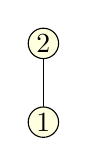
\begin{tikzpicture}
	\begin{pgfonlayer}{main}
		\node [style=inner] (0) at (0, 0) {$1$};
		\node [style=inner] (2) at (0, 1) {$2$};
	\end{pgfonlayer}
	\begin{pgfonlayer}{bg}
		\draw (2.center) to (0.center);
	\end{pgfonlayer}
\end{tikzpicture}\quad
\mathsymbol{.6}{T=}
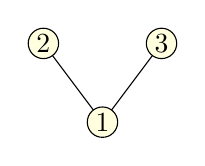
\begin{tikzpicture}
	\begin{pgfonlayer}{main}
		\node [style=inner] (0) at (0, 0) {$1$};
		\node [style=inner] (1) at (-.75, 1) {$2$};
		\node [style=inner] (3) at (.75, 1) {$3$};
	\end{pgfonlayer}
	\begin{pgfonlayer}{bg}
		\draw (1.center) to (0.center);
		\draw (0.center) to (3.center);
	\end{pgfonlayer}
\end{tikzpicture}
\]
then we have that  
\[
\mathsymbol{.6}{T\circ_1 S \; =} \;
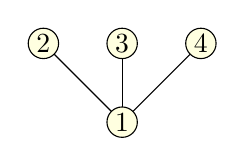
\begin{tikzpicture}
	\begin{pgfonlayer}{main}
		\node [style=inner] (0) at (0, 0) {$1$};
		\node [style=inner] (1) at (-1, 1) {$2$};
		\node [style=inner] (2) at (0, 1) {$3$};
		\node [style=inner] (3) at (1, 1) {$4$};
	\end{pgfonlayer}
	\begin{pgfonlayer}{bg}
		\draw (1.center) to (0.center);
		\draw (2.center) to (0.center);
		\draw (0.center) to (3.center);
	\end{pgfonlayer}
\end{tikzpicture}
\;\mathsymbol{.6}{+}\quad
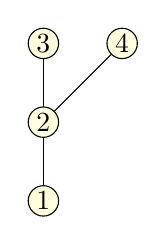
\begin{tikzpicture}
	\begin{pgfonlayer}{main}
		\node [style=inner] (0) at (0, 0) {$1$};
		\node [style=inner] (1) at (0, 1) {$2$};
		\node [style=inner] (2) at (0, 2) {$3$};
		\node [style=inner] (3) at (1, 2) {$4$};
	\end{pgfonlayer}
	\begin{pgfonlayer}{bg}
		\draw (2.center) to (1.center);
		\draw (1.center) to (0.center);
		\draw (1.center) to (3.center);
	\end{pgfonlayer}
\end{tikzpicture}
\;\mathsymbol{.6}{+}\quad
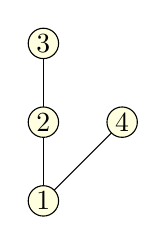
\begin{tikzpicture}
	\begin{pgfonlayer}{main}
		\node [style=inner] (0) at (0, 0) {$1$};
		\node [style=inner] (1) at (0, 1) {$2$};
		\node [style=inner] (2) at (0, 2) {$3$};
		\node [style=inner] (3) at (1, 1) {$4$};
	\end{pgfonlayer}
	\begin{pgfonlayer}{bg}
		\draw (2.center) to (1.center);
		\draw (1.center) to (0.center);
		\draw (0.center) to (3.center);
	\end{pgfonlayer}
\end{tikzpicture}
\;\mathsymbol{.6}{+}\quad
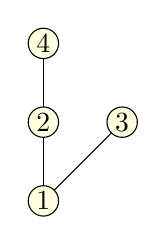
\begin{tikzpicture}
	\begin{pgfonlayer}{main}
		\node [style=inner] (0) at (0, 0) {$1$};
		\node [style=inner] (1) at (0, 1) {$2$};
		\node [style=inner] (2) at (0, 2) {$4$};
		\node [style=inner] (3) at (1, 1) {$3$};
	\end{pgfonlayer}
	\begin{pgfonlayer}{bg}
		\draw (2.center) to (1.center);
		\draw (1.center) to (0.center);
		\draw (0.center) to (3.center);
	\end{pgfonlayer}
\end{tikzpicture}\mathsymbol{.6}{.}
\]
\end{tenumerate}
\subsection{Exercises}

 \begin{question}
 Follow the lecture notes and read about the
 partial definition of an operad (and what
 a Markl operad is). Show that a unital
 pseudo-operad is the same as a unital 
 May operad. 
 \end{question}
 
 \begin{question}
Define the category of collections
in $\mathsf{Vect}$
using the biased approach and the 
unbiased approach (this requires considering
\emph{totally ordered} sets instead of sets,
and their order preserving bijections. We will
write them with calligraphic letters but
use subscripts, so $\mathcal X$ has ns
components $\{\mathcal X_n\}_{n\geqslant 1}$.

\begin{enumerate}
\item Show
that it supports a non-symmetric Cauchy
product given by 
\[ (\mathcal{X}\otimes\mathcal{Y})_n =
  \bigoplus_{i+j=n} \mathcal{X}_i\otimes
   	\mathcal{Y}_j.\]
   	
   	\item Use this and the unbiased approach to 
   	argue that the ns counterpart of a
   	`subset of $I$' is an interval:
   	a totally ordered subset of $I$ of the
   	form $[i,j] = \{ x\in I : i\leqslant x \leqslant j\}$.
 \item Use the previous item to define the
 non-symmetric composition of ns collections.
 Define the generating function associated
 to a collection, and show it behaves
 well with respect to the products above. 
\end{enumerate}
\end{question}

\begin{question}
Since every finite totally ordered set
is, in particular, a finite set (and
every order preserving function is a
fortiori a function) there is a 
map of categories 
$ \mathsf{FinOrd}^\times \longrightarrow
 	\mathsf{FinSet}^\times$
which induces a map that `forgets the
symmetries' ${}_\Sigma\mathsf{Mod}	\longrightarrow\mathsf{Coll}$. 
Show that there is a functor that assigns
a ns sequence $\mathcal{X}$ to the 
sequence $\mathcal{X}_\Sigma(n) =
\kk S_n\otimes \mathcal{X}_n$.  Show that it is
left adjoint to the forgetful functor and that it is monoidal. 
\end{question}
 
\begin{question}
Describe the associator for $\circ_\Sigma$ in the
category of differential graded collections. 
In particular,
write down the signs explicitly. Explain
how this is related to the signs
in the parallel composition axiom
for \emph{graded operads} that read as follows:
for elements $f,g$ and $h$
in an operad (of homogeneous arities)
and $\delta = i-j+1$, we have that
\[ 
(f \circ_j g) \circ_i h  = 
 	\begin{cases} 
 		(-1)^{|g||h|}
 		 (f \circ_i h) \circ_{\ari(f)+j-1} g
 		  	& \delta \leqslant 0  \\
 		 \phantom{(-1)^{|g||h|}(} 	f\circ_j (g \circ_\delta h) &
 		  	\delta\in [1,\ari(g)] \\
 		(-1)^{|g||h|}
   	(f \circ_\delta h) \circ_j g
   		 & \delta > \ari(g).
 		   \end{cases}
 		 \]
\end{question}

\begin{question}
A (unital associative) monoid $x$ in a monoidal category 
$(\mathcal C,\otimes,\alpha,\rho,\lambda,1)$ is an object
along with maps $\mu: x\otimes x\to x$ and $\eta : 1
 \longrightarrow x$ such that $\mu$ is associative, 
 that is $\mu (\mu\otimes 1) = \mu(1\otimes \mu)
 \alpha_{x,x,x}$, and unital for
$\eta$, that is $\mu(\eta\otimes 1)=\rho_x$
and $\mu(1\otimes \eta) = \lambda_x$.
Show that a $\Sigma$-operad is exactly the
same as a monoid in $({}_\Sigma\mathsf{Mod},\circ_\Sigma)$.
\end{question}

\begin{question}
We write $\mathsf{End}$ for
 category of endofunctors of $\mathsf{Vect}$. Show
 that there is a \emph{monoidal}
 functor $S:{}_\Sigma\mathsf{Mod}
 \longrightarrow \mathsf{End}$ that assigns
 $\mathcal{X}$ to $V\longmapsto \bigoplus_{n\geqslant 0} \mathcal{X}(n)\otimes_{\Sigma_n} V^{\otimes n}$.
 It is called the \emph{Schur functor} associated
 to $\mathcal{X}$. The endofunctors in the essential
 image of $S$ are called \emph{analytic}.
\end{question}

\begin{question}
	 If $\mathcal{X}$
	 is a symmetric sequence, describe the $\Sigma_n$
	 action on $\mathcal{X}^{\otimes n}$ where
	 $\otimes$ is the Cauchy product. Observe that
	 it commutes with the $\Aut(I)$ action on 
	 $\mathcal{X}^{\otimes n}(I)$.
\end{question}
	 
\begin{question}
Define ${}_\Sigma\mathsf{Mod}(\CC)$
for any symmetric monoidal category $(\CC,\otimes,1)$
(such as the category of sets, or topological spaces,
or chain complexes, among others) along with
its \emph{symmetric composition product}
 $-\circ_\Sigma - $.
 \end{question}
 
\begin{question} Prove that non-unital Markl operads
and non-unital May operads differ.
To do this, consider the non-unital ns operad
$\PP$ such that $\PP(2)$ and $\PP(4)$
are its only non-zero components, and are
both one dimensional, and define
\[ \gamma : \PP(2)\otimes \PP(2)\otimes \PP(2)
 	\longrightarrow \PP(4) \]
to be an isomorphism, and set all other maps to zero. 
Check that $\PP$ is a May operad, and
show that $\PP$ is not a Markl
operad by exploring the consequences
of the equality
\[ \mu(\mu,\mu) = (\mu \circ_2\mu)\circ_1 \mu \]
in any Markl operad.
\end{question}

\begin{question}
 Check that examples (1), (2), (4), (5) are indeed all operads.
\end{question}
%
%\begin{question}
%Follow these steps to construct the
%Stasheff operad as a sequence of 
%convex polytopes $K_2',K_3',\ldots$
%for which the boundary of $K_{n+1}'$
%is a union of products $K_{r+1}'\times
%K_{s+1}'$ with $r+s=n$ indexes by
%planar rooted trees with two internal
%vertices.
%\end{question}
%\begin{enumerate}
%\item Let us write $T_n$ for the collection
%of planar rooted \emph{binary} 
%trees with $n+1$ leaves, which we 
%order from left to right. Explain how
%this gives a total order on the vertices,
%which we will thus call $1,\ldots,n$.
%\item  For
%each $t\in T_n$ and each vertex $i$ of
%$t$, let $L(i)$ denote the number of paths
%from $i$ to a leaf of $t$ going through
%its left child, and let $R(i)$ denote
%the the number of paths
%from $i$ to a leaf of $t$ going through
%its right child. We define
%\[ x(t) = (L(1)R(1),\ldots,L(n)R(n))
%	\in \mathbb N^n. \]
%Show that $x(t)$ always lies in the
%hyperplane $x_1+\cdots x_n = \binom{n}{2}$.	
%We write $K_{n+2}'$ for the convex hull of 
%the points $\{ x(t) : t\in T_n \}$.
%\emph{Hint.} Any planar binary rooted tree
%$t$ decomposes into a left tree $L_t$
%and a right tree $R_t$ by looking at the
%children of the unique child of the root.
%Express $W(t) = \sum_{i=1}^n x(t)$ in terms of $W(R_t)$ and $W(L_t)$.
%
%\item 
%Show that the polytope $K_{n+2}'$ 
%is of dimension $n$, 
%and its $k$-cells for $k\in [n]$
%are in bijection with planar rooted
%trees with $n-k+1$ internal vertices
%and $n+2$ leaves. Conclude, in particular,
%that its codimension one faces are
%in bijection with planar rooted trees
%with $2$ internal vertices and $n+2$
%leaves.
%
%\item Suppose that $t$ has $r+1$
%leaves and that $t'$ has $s+1$ leaves,
%and consider the grafting $t\circ_i t'$.
%We define $x(t)\circ_i x(t')$ by
%$x(t\circ_i t')$. Show that this
%defines a map
%\[\circ_i :  K_{r+1}'\times K_{s+1}' 
%	\longrightarrow K_{r+s+1}'.\]
%\item Show the maps above give the
%collection $\{K_{n+2}'\}_{n\geqslant 0}$
%the structure of a ns operad.
%\end{enumerate}

\begin{question}
Suppose that $T\in\mathsf{RT}(n)$ and
that $T'\in \mathsf{RT}(m)$, where $\mathsf{RT}$
is the symmetric collection
 of rooted trees of Lecture 1,
and let $\mathrm{In}(T,i)$ denote the
set of incoming edges of $T$ at the
vertex labeled $i$. For each function
$f: \mathrm{In}(T,i)\longrightarrow [m]$,
define the tree $T\circ_i^f T'$ by
replacing vertex $i$ of $T$ by $T'$ and
attaching the loose incoming edges of 
vertex $i$ to the vertices of $T'$
according to the map $f$: the edge
$e\in \mathrm{In}(T,i)$ is attached
to vertex $f(e)\in T'$. Finally,
define $T\circ_i T'$ by taking the
sum through all possible functions
$f$. Show that this gives $\mathsf{RT}$
the structure of a unital pseudo-operad,
and thus of a usual operad, with unit
the tree with no edges and one vertex.
\end{question}


\begin{question}
 Describe the operation $T\star T' = S(T,T')$ where
$S$ is the rooted tree 
\[
\mathsymbol{.6}{S=} 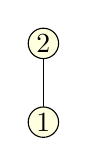
\begin{tikzpicture}
	\begin{pgfonlayer}{main}
		\node [style=inner] (0) at (0, 0) {$1$};
		\node [style=inner] (2) at (0, 1) {$2$};
	\end{pgfonlayer}
	\begin{pgfonlayer}{bg}
		\draw (2.center) to (0.center);
	\end{pgfonlayer}
\end{tikzpicture}
\]
above in terms of 
insertions of $T'$ in $T$ and regrafting of incoming 
edges. Show that it satisfies the following \emph{pre-Lie
identity}:
\[
  (T\star T')\star T'' -  T \star (T' \star T'' ) =
    (T\star T'')\star T' -  T \star (T'' \star T' ) 
 	\]
 	by explicitly interpreting the left hand side in
 	terms of certain insertions of $T'$ and $T''$ in $T$,
 	and showing the resulting sum of trees is symmetric
 	in $T'$ and $T''$.

\end{question}

\begin{question}
Suppose that $\mathcal P$ is an operad
and that $\mathcal X\subseteq \mathcal P$
is a symmetric subsequence. We say
$\mathcal X$ generates $\mathcal P$
if every element of $\mathcal P$ is
an iterated composition of elements of
$\mathcal X$. 
Show that the rooted trees operad 
$\mathrm{RT}$ 
is generated by the symmetric subsequence
generated by the rooted tree $S$ of the
previous exercise, which spans
the regular representation of
$S_2$. Follow these steps:
\end{question}
\begin{tenumerate}
\item Suppose that $T$ is an $n$-rooted tree
and let $J$ be a subset of $[n]$ corresponding
to leaves of $T$ that are the children of a
vertex $i\in T$. Let $T'$ be the
tree obtained by erasing all these leaves
and replacing the vertex label by a new
symbol $\ast$, and let $T''$ be the rooted
tree with root $i$ and children labeled
by $J$. Show that $T'\star_\ast T'' = T$.
\item Use the above and induction on the
number of vertices to show it suffices to prove
the claim for the corollas, that is, trees with
one internal root vertex.
\item Let us write $T_n$
for the operation in $\mathsf{RT}(n)$
corresponding to a corolla with root $1$,
so in particular $T_2 = S$.
Show that 
\[ 
T_n = 
 T_2\star T_{n-1} - 
  	\sum_{i=1}^{n-1} (T_{n-1}\star T_i)\sigma_i
\]
where $\sigma_i = (i+1,i+2,\ldots,n)\in S_n$
is a cycle, and use this to conclude.
\end{tenumerate}

\emph{Note.} The operation $T_n$ is usually
denoted $\{x_1; x_2,\ldots,x_n\}$ and is called
a \emph{symmetric brace}, and the equation
above is usually written in the form
\[ 
\{x_1; x_2,\ldots,x_n\} = 
 \{\{x_1; x_2,\ldots,x_{n-1}\}; x_n\}
 - \sum_{i=1}^{n-1} \{ x_1; x_2,
 \ldots, x_{i-1}, \{x_i ; x_n \},
 x_{i+1},\ldots,x_{n-1}\}.
 \]
 
 \begin{question}
 Let $\mathcal X$ be a symmetric sequence,
 and define the derivative $\partial\mathcal X$ 
 of $\mathcal X$ to be symmetric sequence
 with $(\partial\mathcal X)(I) = \mathcal X(I^*)$
 where $I^* = I \sqcup \{ I \}$. Note that
 $S_I$ acts on $I^*$ fixing the element $I$.
 Show that $(\partial \mathcal X)(n)$ 
 is isomorphic to the restriction of $\mathcal{X}(n+1)$ to $S_n = \mathrm{Fix}(n+1)$, and
 conclude that 
 \[ \partial_z f_{\mathcal X}(z) = 
  			f_{\partial\mathcal X}(z). \]	
  Let $s$ be the sequence of singletons and
  define the pointing of operation by
  $\mathcal X^\bullet = s\otimes_\Sigma \partial   \mathcal{X}$. Determine the representation
  $\mathcal{X}^\bullet(n)$ in terms of
  $\mathcal{X}(n)$. 
 \end{question}

\afterpage{\blankpage}
\newpage

\section{Free operads and presentations}\label{lecture:freeops}

\textbf{Goals.} We will define algebraic operads
by generators and relations, and with this at
hand define quadratic and quadratic-linear
presentations of operads. 

\subsection{Trees}

Operads and their kin are gadgets modeled after
combinatorial graph-like objects. Operads themselves are modeled after
rooted trees, so it is a good idea to have a concrete definition of 
what a rooted tree is. We will also consider planar rooted trees,
and trees with certain decorations, so it is a good idea to digest
the definitions carefully to later embellish them.

A rooted tree $\tau$ is the datum of a finite set $V(\tau)$
of vertices along with a partition $V(\tau) = 
\mathrm{Int}(\tau)\sqcup L(\tau) \cup R(\tau)$,
where the first are the \emph{interior} vertices, $L$ are the leaves, and $R(\tau)$ is
a singleton, called the root of $\tau$. We also require there is 
a function $p :V(\tau)\smallsetminus R(\tau) \longrightarrow V(\tau)$,
describing the edges of $\tau$, 
with the following properties: call a vertex $v\in V(\tau)$ a child 
of $w\in V(\tau)$ if $v\in p^{-1}(w)$. Then:
\begin{tenumerate}
\item The root $r\in R(\tau)$ has exactly one child.
\item The leaves of $\tau$ have no children.
\item For each non-root vertex $v$ there exist a unique sequence
$(v_0,v_1,\ldots,v_k)$ such that $p(v_{i-1}) = v_{i}$ for $i\in [k]$
with $v_0 = v$ and $v_k = r$.
\end{tenumerate}
We will call a non-leaf vertex that has no children a \emph{stump}
(or an endpoint, or a cherry-top).
A tree is reduced if has no stumps. We say it is 
series-reduced if all of its non-root and
non-leaf vertices have at least two children. We will also call
the root the (unique) \emph{output vertex} of $\tau$, and the leaves
the \emph{input vertices} of $\tau$. 

A planar rooted tree is a rooted tree $\tau$
along with a linear order in each of the fibres
of the parent function $p$ of $\tau$. In short,
the children of each vertex are linearly ordered,
so we are effectively considering a drawing of
$\tau$ in the plane, where the clockwise
orientation gives us the order at each
vertex. 

Two rooted trees $\tau$ and $\tau'$ are isomorphic
if there exists a bijection $f : V(\tau) \longrightarrow 
V(\tau')$ that preserves the root, the input vertices and the
interior vertices, so that $p'\circ f = p$ where we
also write $f$ for the induced bijection $f : V(\tau)\smallsetminus r \longrightarrow 
V(\tau')\smallsetminus r'$. Two planar rooted trees
are isomorphic if in addition $f$ respects the linear order
at each vertex.

For example, consider the rooted tree $\tau$ with
$V = \{1,2,3\}\cup \{4,5\}\cup \{0\}$, that is,
three leaves, two interior vertices and the root.
Then the choice of $p : [5] \to \llbracket 5 \rrbracket$ 
with $p(\{1,2\}) = 4$, $p(\{3,4\}) = 5$, $p(5) = 0$
gives a tree isomorphic to the one with 
with $p(\{1,2\}) = 3$, $p(\{3,4\}) = 5$, $p(5) = 0$.
On the other hand, if we consider the vertices linearly
ordered by their natural order, these two planar rooted trees 
are no longer isomorphic. 

\begin{definition}
For a finite set $I$, an $I$-labeled tree $T$
is a pair $(\tau,f)$ where $\tau$ is a 
reduced rooted tree, along with
a bijection $f : I \longrightarrow L(\tau)$.
Two $I$-labeled trees $T$ an $T'$ are isomorphic
if there exists a pair $(g,\sigma)$ where
$g$ is an isomorphism between $\tau$ and $\tau'$
and $\sigma$ is an automorphism of $I$ such that
$g\mid_{L(\tau)}\circ f = \sigma\circ f'$. 
\end{definition}

Suppose that $(\tau,f)$ is an $I$-tree and that
$(\tau',f')$ is a $J$-tree, and that $i\in I$. We define
$K=I\cup_i J = I\sqcup J \smallsetminus i$ and the
$K$-tree $\tau\circ_i \tau'$ as follows:
\begin{tenumerate}
\item Its leaves are $L(\tau\circ_i \tau') = L(\tau)\sqcup L(\tau')\smallsetminus f^{-1}(i)$.
\item Its internal vertices are $V(\tau)\sqcup V(\tau')$, with
root $r$. 
\item The parent function $q$ is defined by declaring that:
	\begin{titemize} 
	\item $q$ coincides with $p$ on $V(\tau)$, 
	\item $q(w) = p(f^{-1}(i))$ if
$w$ is the unique children of the root of $\tau'$, 
	\item  $q$
coincides with $p'$ on $V(\tau')\smallsetminus \{r',w\}$.
\end{titemize}
\item The leaf labeling is the unique bijection $L(\tau\circ_i \tau') \longrightarrow I\circ_i J$ extending $f$ and $f'$.
\end{tenumerate} 

\subsection{Tree monomials}
Let us now consider an 
(unbiased) reduced symmetric sequence $\XX$ which
we will think of as an \emph{alphabet}. A tree monomial in the
alphabet $\XX$ 
is a pair $(\tau,x)$ where $\tau$ is a reduced rooted
tree and $x : \mathrm{Int}(\tau) \longrightarrow \XX$ is a map
with the property that $x(v) \in \XX(p^{-1}(v))$. Observe that
reduced sequences and reduced trees correspond to each other, in the
sense that with this definition we can only decorate a stump
of $\tau$ with an element of $\XX(\varnothing)$. 

An $I$-labeled
$\XX$-tree $T$ is a triple $(\tau,x,f)$ where $(\tau,f)$ is $I$-labeled
and $(\tau,x)$ is an $\XX$-tree. We will say that $(\tau,x,f)$
is a (symmetric) tree monomial if $\XX$ is symmetric. If it
is just a collection, we will say that $(\tau,x,f)$ is a
ns tree monomial. In particular, if $T$ is an $I$-labeled
tree, and if $\sigma \in \Aut(I)$, there is another 
$I$-labeled tree $\sigma(T)=(\tau,f\sigma^{-1})$. 


Suppose that $T = (\tau,x,f)$ is a tree monomial on an
alphabet $\XX$, and let us pick a vertex $v$ of $\tau$
and a permutation $\sigma$ of the set $C = p^{-1}(v)$ of
children of $v$. We define the tree $\tau^\sigma$ as
follows: the datum defining $\tau$ remains unchanged
except $p$ is modified to $p^\sigma$ so that 
\[ p^\sigma(w) = 
\begin{cases}
 p(w) & \text{if $p^2(w)\neq v$} \\
 p(\sigma^{-1}(w')) & \text{if $p(w)=w'\in C$}.
\end{cases}
\]
Briefly, we just relabel the vertices of $\tau$
using $\sigma$. With this at hand, we define
$T^\sigma$ to be the tree monomial with underlying 
tree $\tau^\sigma$ and with $x$ modified to $x^\sigma$ so that
\[ x^\sigma(w) = 
\begin{cases}
 \sigma x(v) & \text{if $v=w$,} \\
 x(\sigma^{-1}(w')) & \text{if $p(w)=w'\in C$}.
\end{cases}
\]
Note that it is possible some children of $v$ are
leaves, in which case the definitions make sense if
we think of leaves as decorated by the unit of
$\kk$. 

\begin{example}
Let us consider the alphabet 
$\XX = \XX(2) = \{\ast \}$ where
the unique operation is antisymmetric.
Then we have the following equalities
of symmetric tree monomials:
\[ 
	\leftc{}{}{2}{1}{3}  \mathsymbol{1.5}{=}
\rightc{}{}{3}{1}{2}  
   \mathsymbol{1.5}{=-}
 {\leftc{}{}{1}{2}{3}}
  \mathsymbol{1.5}{.}\]
 
\end{example}


Let us now define for each $n\geqslant 1$ the
space $\FF_\XX(I)$ as the span of all tree monomials
$T = (\tau,f,x)$ on $\XX$ with leaves labeled by $I$,
modulo the subspace generated by all elements of the form
\[ R(T,v,\sigma) = T - T^\sigma \]
where $\sigma$ ranges through $\Aut(p^{-1}(v))$ as
$v$ ranges through the vertices of $\tau$. In case
all children of $v$ are leaves, this is saying that
the tree where $x_v$ is replace by $\sigma(x_v)$
is equal to the tree where the leaves of $T$ that are
children of $v$ are relabeled according to $\sigma$.
We also require that tree decorations behave like
tensors, so that $T = T_1+T_2$ if the decoration
of $T$ at a vertex $v$ is of the form $x_1 + x_2$
and for $i\in [2]$ the tree $T_i$ coincides with
$T$ except that it is decorated by $x_i$ at $v$.



\subsection{The free operad}
An algebraically inclined way to construct
(algebraic) operads is through generators and
relations. There is a forgetful functor
from the category of operads to the category
of collections. In general, it admits a left
adjoint, which is the free operad functor.

\begin{definition}
The \emph{free symmetric operad} on $\XX$ is the
symmetric sequence $\FF_\XX$ along with the composition
law obtained by grafting of trees. More precisely,
suppose that $T\in \FF_\XX(I)$ and that $T'\in\FF_\XX(J)$,
and that $i\in I$. We define $T'' =T\circ_i T' \in 
\FF_\XX(I\cup_I J)$ by taking its underlying labeled
tree to be $\tau\circ_i \tau'$, and by decorating it
in the unique way which extends the decorations of 
$T$ and $T'$.
\end{definition}

The following lemma shows that this indeed defines an operad.

\begin{lemma}
Tree grafting respects both $I$-tree 
isomorphisms and the relations $T\sim T^\sigma$
above, and hence is well defined on $\FF_\XX$.
\end{lemma}

\begin{proof}
This is Exercise~\ref{ex:grafting}.
\end{proof}

The functor $\XX\longmapsto \FF_\XX$ is in fact a \emph{monad},
the monad of rooted trees,
which gives us the definition of an operads alluded to 
in Lecture~\ref{lecture:theintro}. The
advantage of this `monadic approach' is its 
flexibility, which allow us to define other
operad like structures, like the ones 
mentioned in the introduction.
In this direction, a curious reader 
can consider the following 
equivalent definition; see also Exercise~\ref{ex:colim}.

\begin{definition}
The free operad generated by a symmetric
collection $X$ is defined inductively by
letting  $\FF_{0,X}=\kk$ be spanned
by the `twig' (tree with no vertices and one edge)
in arity zero and
\[ \FF_{n+1,\XX} = \kk\oplus (\XX\circ  \FF_{n,\XX} ), \]
and finally by setting
$\FF_\XX = \varinjlim_n \FF_{n+1,\XX}$.
The composition maps are defined by induction,
and the axioms are also checked by induction.
\end{definition}

Intuitively, the previous definition says that an element of
$\FF_\XX$ is either the twig, or corolla
with $n$ vertices decorated by $\XX$, whose leaves
have on them an element of $\FF_\XX$. The
final shape of $\FF_\XX$ will however
depend on the symmetric structure of $ \XX$. 
 \subsection{Exercises}


 
 \begin{question}
Let $\XX$ be a collection such that $\underline{\XX} = 
\XX(2)$. Compute a basis of tree monomials 
for the free operad over
$\XX$ in case $\XX(2)$ is:
\begin{tenumerate}
\item The regular representation of $S_2$.
\item The sign representation of $S_2$.
\item The trivial representation of $S_2$. 
\end{tenumerate} 
In all cases, decompose the $S_3$-module $\mathcal{F}_\XX(3)$
into irreducible representations.
\end{question}


\begin{question}\label{ex:grafting}
Show that tree grafting respects both $I$-tree
isomorphism and the relation $T\sim T^\sigma$,
and hence descends to $\FF_\XX$.
\end{question}

\begin{question}
Suppose that $\XX$ is an alphabet (in sets) that is
finite in each arity and such that $\XX(n) = \varnothing$
for $n=0,1$. Show that $\mathcal{F}_\XX$ is finite
in each arity. 
\end{question}
 
\begin{question}
Define non-symmetric tree monomials over a ns alphabet
$\XX$ and thus define the free \emph{non-symmetric}
operad over a collection $\XX$.
\end{question}

\begin{question}\label{ex:colim}
Read the statement and proof of \emph{Theorem 5.4.2} in
`Algebraic Operads' that the colimit construction briefly
described in the lecture notes does give the free
operad on a symmetric collection.
\end{question}

\begin{question}
Consider the map from ns collections to symmetric sequences
that assigns $\XX$ to $\Sigma\otimes \XX$ such that
$(\Sigma\times \XX)(n) = \Sigma_n\times \XX(n)$ with its
corresponding symmetric group action. What is the relation
between the free ns operad on $\XX$ and the free symmetric
operad on $\Sigma\times \XX$?
\end{question}

\begin{question}
Let $V$ be an $S_2$-module, and let $\XX$ be the
symmetric collection with $\XX(2) = V$ and zero
everywhere else. Show that $\mathcal{F}_\XX(3)$
consists of three copies of $V^{\otimes 2}$ and
describe explicitly the action of $S_3$ on it.
\end{question}

\begin{question}
Show that the construction of the free operad we carried
out during \textbf{Lecture~2} indeed defines the free
operad on $\XX$ where $i:\XX \longrightarrow \mathcal F_\XX$
sends an element $x\in \XX(I)$ to the corolla whose unique
internal vertex is labeled by $x$ (and whose
leaves are labeled by $I$). 
\end{question}

% \begin{question}
% Follow the lecture notes and read about 
% weight gradings and the canonical weight
% grading on a free operad. 
% \end{question}
\afterpage{\blankpage}
\newpage

\section{Quadratic operads}\label{lecture:quadraticops}

 \textbf{Goal.} Introduce weight graded gadgets,
 define operads by generators and relations, and
 introduce quadratic operads. Give plenty of examples
 of `real life' quadratic operads to work on:
 Hilbert series, Koszul dual, bar construction. 
 
 \subsection{Weight gradings and presentations}
 The notion of a quadratic operad is based on the observation
 every free operad has a canonical `weight grading' by the
 number of internal vertices of a tree. Let us make this
 precise.
 
\begin{definition}
A symmetric sequence $\XX$ is weight graded if for
each finite set the component $\XX(I)$ admits a 
decomposition $\XX(I) = \bigoplus_{j\geqslant 0}
\XX^{(j)}(I)$. A symmetric operad $\PP$ is weight
graded if its underlying symmetric sequence
is weight graded and its composition maps
preserve the weight grading.
\end{definition}

Thus, a weight graded operad must have composition maps 
of the form
\[ \PP^{(a)}(k) \otimes 
	\PP^{(b_1)}(n_1) \otimes \cdots \otimes \PP^{(b_k)}(n_k)
	 	\longrightarrow \PP^{(b)}(n) \]
where $b=b_1+\cdots+b_k$ and $n = n_1+\cdots+n_k$. In the
case we consider partial composition maps, observe we have
instead maps of the form
\[\circ_i :  \PP^{(a)}(m)\otimes  \PP^{(b)}(n)
	\longrightarrow  \PP^{(a+b)}(m+n-1). \] 
The free operad $\FF_\XX$ is weight graded by the number
of internal vertices of a tree (that is, we put $\XX$ in
weight one, and extend the weight to trees by counting 
occurrences of elements of $\XX$. More generally, if
$\XX$ admits a weight grading, then $\FF_\XX$ inherits
this weight grading: the weight of a tree monomial is the
sum of the weight of the decorations of its vertices,
 and we write $\FF_\XX^{(n)}$ for the
homogeneous component of weight $n\in\NN_0$. If we do
not specify a weight grading on $\FF_\XX$, we will 
always assume we are taking the canonical weight grading above.


\begin{definition} An ideal in an operad $\PP$
is a subcollection $\mathcal{I}$ for which
 $\gamma(\nu_0;\nu_1,\ldots,\nu_k)\in \mathcal{I}$ if at least one $\nu_i$ is in 
$\mathcal I$ for some $i\in \underline{k}$.
The quotient of $\PP/\mathcal{I}$ is again an
operad, called the quotient of $\PP$ 
by $\mathcal{I}$. Every subcollection $\RR$
of $\PP$ is contained in a smallest
ideal, called the \emph{ideal generated by $\RR$}.
\end{definition}

The notion of ideals and of free operads allow us
to define operads by generators and relations.

\begin{definition}
We write $\FF(\XX,\RR)$ for the quotient of 
$\FF_\XX$
by the ideal generated by a subcollection $\RR$
of $\FF_\XX$. 
 We say $\PP$ is presented by generators
$\XX$ and relations $\RR$ if there is an
isomorphism $\FF(\XX,\RR) \longrightarrow
\PP$.
\end{definition}

Note that if $\PP$ is symmetric, the definition
requires that $\mathcal{I}$ be stable under
the symmetric group actions, so we may 
sometimes specify $\RR$ by a generating set 
only, and understand
that $(\RR)$ is generated by the $\Sigma$-orbit
of $\RR$.

\bigskip

\textbf{Some examples.}
To illustrate the definitions above, let us
give three examples of algebraic operads whose
associated algebras are probably well known
to the reader: 
\begin{tenumerate}
\item The associative operad is generated by a 
binary operation $\mu$ generating the regular
representation of $S_2$ subject to the relation
$\mu\circ_1 \mu = \mu \circ_2 \mu$. 
\item The commutative operad is generated by a 
binary operation which instead generates the
trivial representation of $S_2$ and is
also associative. Both of this 
and the previous
example arise as the linearization of a set operad.
\item 
The Lie operad is generated by a single binary 
operation $\beta$ that generates the sign 
representation of $S_2$ subject to the only
relation
$(\beta \circ_1 \beta)(1+\tau+\tau^2) = 0$
where $\tau = (123)\in S_3$ is the $3$-cycle. 
\end{tenumerate}
We write these operads $\mathsf{As},\mathsf{Com}$
and $\mathsf{Lie}$ and, following J.-L. Loday,
call them the \emph{three graces}. We have that
\[ \As(n) = \kk S_n,\quad
 	\Com(n) = \kk, \quad
 	 \Lie(n) = \operatorname{Ind}_{\mathbb Z/n}^{S_n} \kk_\zeta \] 
 where $\kk_\zeta$ is a character of $\mathbb Z/n$
 for a primitive $n$th root of the unit. Concretely,
 the last equality is stating that if we fix a primitive
 $k$th root of unity $\zeta_k$, and if we let $\rho_k$ be
 the standard $k$-cycle of $S_k$, the free Lie
 algebra $L(V)\subseteq T(V)$ identifies  
 in each weight degree $k$ with those $v
 \in V^{\otimes k}$ such that $\rho_k v = \zeta_k v$; see~\cite{Klyachko1975,MO187545}.
 
\begin{note} It is not always advantageous
to define an operad by generators and relations:
the operad pre-Lie can be defined explicitly
in terms of labeled rooted trees and a grafting
operation, as done by Chapoton--Livernet, and
this `presentation' is very useful in practice,
for example, to show that the pre-Lie operad
is Koszul.
\end{note}

\subsection{Quadratic operads}
An operad $\PP$ is \emph{quadratic} if it admits a presentation
$\FF(\XX,\RR)$ where $\RR \subseteq \FF(\XX)^{(2)}$. 
That is, $\PP$ is generated by some collection of
operations $\XX$ and all its defining relations are of the form
\[ \sum \lambda_{\mu,\nu}^i\cdot \mu \circ_i \nu = 0  \] 
where $\ari(\mu)+\ari(\nu)$ is constant. An operad is
\emph{binary quadratic} if moreover $\XX = \XX(2)$ or,
what is the same, all the generating operations of $\PP$
are of arity two (binary). 
 A \emph{quadratic-linear presentation} of an operad $\PP$
is a presentation $\FF(\XX,\RR)$ of $\PP$ where $\RR 
\subseteq \XX \oplus \FF(\XX)^{(2)}$. That is, it is
a presentation of the form
\[ \sum \lambda_{\mu,\nu}^i \cdot\mu \circ_i \nu 
 + \sum \lambda_\rho \cdot \rho = 0   \] 
 where $\ari(\mu)+\ari(\nu) = \ari(\rho)+1$ is constant.
 Every operad admits a quadratic-linear
presentation, albeit with possibly with infinitely many generators, 
We point the reader to~\cite{Loday2012}*{Section 7.8} for a comprehensive treatment of operads
with quadratic linear relations.
 
 Let us define a quadratic datum to be a pair $(\XX,\RR)$
 where $\XX$ is a symmetric sequence and $\RR\subseteq
 \FF_\XX^{(2)}$. A map of quadratic data $(\XX_1,\RR_1) 
 \longrightarrow (\XX_2,\RR_2)$ is a map $\XX_1
 \to \XX_2$ of symmetric sequences for which the induced
 map on free operads sends $\RR_1$ to $\RR_2$. The 
 assignment $(\XX,\RR) \longrightarrow \FF(\XX,\RR)$
 defines a functor from the category of quadratic data
 to the category of quadratic operads.
 
 %%Exercise: find two different QD giving same operad.
 \bigskip
 
\textbf{More examples.} The presentations of the 
associative, commutative and Lie operad above are
quadratic. The following are also quadratic operads:

\emph{The Gerstenhaber operad}. The symmetric operad
$\mathsf{Ger}$ and its cousin,
the Poisson operad $\mathsf{Poiss}$ belong to the two parameter
family $\mathsf{Poiss}(a,b)$ of binary quadratic operads generated
by two operations $x_1x_2$ and $[x_1,x_2]$ of respective degrees
$a$ and $b$, so that
the first is commutative associative, the second is a Lie
bracket, and they satisfy the Leibniz rule. With this
at hand $\mathsf{Ger} =\mathsf{Poiss}(0,-1)$ while  
$\mathsf{Poiss} = \mathsf{Poiss}(0,0)$.

\smallskip

\emph{The pre-Lie operad}. The operad $\mathsf{PreLie}$ and its
quotient, the Novikov operad $\mathsf{Nov}$, are quadratic
binary operads generated by a single operation $x_1\circ x_2$
with no symmetries. The first one is subject to the right-symmetry
condition for the associator
\[ 
x_1\circ (x_2\circ x_3) - (x_1\circ x_2)\circ x_3	=
x_1\circ (x_3\circ x_2) - (x_1\circ x_3)\circ x_2.
\]
The second 
operad is obtained by further imposing the left-permutative
relation that 
\[ x_1\circ (x_2\circ x_3) = x_2\circ (x_1\circ x_3).\]
The permutative operad $\mathsf{Perm}$ is the binary
operad generated by a single operation with no symmetries
satisfying the last quadratic equation.

\smallskip

\emph{The operad of totally associative $k$-ary algebras}. 
$\mathsf{tAs}_k$ (and its commutative counterpart). It is generated
by a $k$-ary non-symmetric operation $\alpha$ subject to
the relations $\alpha \circ_i \alpha =\alpha\circ_k \alpha$
for all $i\in \underline{k}$. One can consider $\alpha$ to be
totally symmetric, and obtain the operad of totally
associative commutative $k$-ary algebras.

\smallskip

\emph{The operad of partially associative $k$-ary algebras}.
$\mathsf{pAs}^k$ (and its Lie counterpart). It is generated
by a $k$-ary non-symmetric operation $\alpha$ of degree $k-2$
subject to the single relation
\[ 
	\sum_{i=1}^k (-1)^{(k-1)(i-1)} \alpha\circ_i \alpha = 0.\]
One can consider a $k$-ary totally antisymmetric operation
$\beta$ of degree $1$, and obtain the operad of Lie $k$-algebras, 
which is subject to the single equation
\[
 \sum_{\substack{A\sqcup B = [2k-3] \\
 |A|=k-1,|B|=k-2}}  (\beta\circ_1\beta)\sigma_{A,B} = 0.
 \]

\smallskip

\emph{The operad of anti-associative algebras.} $\mathsf{As}^-$ is
generated by a single operation of degree zero with no symmetries
satisfying the `anti-associative law'
\[ x_1(x_2x_3) + (x_1x_2)x_3 = 0. \]

\subsection{Exercises}


 \begin{question}
During Lecture~\ref{lecture:quadraticops} we introduced the associative and commutative operads
through binary quadratic presentations. Show  that 
for all $n\geqslant 1$ the space $\mathsf{Ass}(n)$ is the
regular representation of $S_n$, and that for 
all $n\geqslant 1$ the space $\mathsf{Com}(n)$ is the 
trivial representation.
\end{question}

\begin{question} Use the presentation of the Poisson operad given
during Lecture~\ref{lecture:quadraticops} to show that $\dim\mathsf{Poiss}(n)\leqslant n!$
for all $n\geqslant 1$\footnote{There are at least three different
ways to show that equality holds.}. 
\end{question}

\begin{question} Let $x_1x_2$ be the associative binary generator of
$\mathsf{Ass}$ and let us consider the operations (which are symmetric
and antisymmetric, respectively)
\[x_1\cdot x_2 = \frac{1}{2}(x_1x_2+x_2x_1), \quad 
	 [x_1,x_2] = \frac{1}{2}(x_1x_2-x_2x_1) 	
	 \]
obtained by `polarization'. Show that the second is a Lie bracket,
and that the first is a commutative (but not associative) product
that satisfies the Leibniz rule for $[x_1,x_2]$, and whose associator
is equal to $[x_2,[x_1,x_3]]$. This is called the \emph{Livernet--Loday
presentation} of the associative operad.
\end{question}

\begin{question} 
During Lecture~\ref{lecture:quadraticops}, we introduced to operad $\mathsf{tCom}_k$ of totally
associative commutative $k$-ary algebras. It is generated by a single
fully symmetric operation $\mu$ or arity $k$ subject to the relations
$\mu\circ_1\mu = \mu\circ_i\mu$
for each $i\in \underline{k}$ (and all its symmetric translates).
Show that $\mathsf{tCom}_k(n)$ is either the one dimensional trivial
representation or zero depending on $n$. What values must
$n$ take so that it is non-zero? 
\end{question}

\begin{question}
The permutative operad $\mathsf{Perm}$ is generated by a single
binary operation $x_1x_2$ with no symmetries which is associative,
and such that
\[ x_1(x_2x_3) = x_2(x_1x_3). \]
Show that $\mathsf{Perm}(n)$ is of dimension $n$ and is
isomorphic as a representation to $\mathrm{Ind}_{S_{n-1}}^{S_n}\mathbb{C}$
where $\mathbb{C}$ is the trivial representation.
\end{question}



We have defined quadratic operads as precisely those
operads presented by (homogeneous) quadratic relations
on some set of generators. Let us explore how to create
maps between them.



\begin{question}
Suppose that $(\mathcal{X},\mathcal{R})$ and $(\mathcal{Y},\mathcal Q)$
are quadratic data. Show that a
map of sequences $f: \mathcal{X} \longrightarrow \mathcal{Y}$
induces a map on the corresponding quadratic operads if and only if
the induced map $F = \mathcal{F}_f$ sends $\mathcal{R}$ to
$\mathcal{Q}$.
\end{question}

\begin{question}
Show that:
\begin{tenumerate}
\item The augmentation map
$\mathbb C S_2\longrightarrow \mathbb C$ (that
sends $1$ and $(12)$ to $1$) induces a surjective map of
operads $\mathsf{Ass}
\longrightarrow \mathsf{Com}$.
\item The inclusion map
$\mathbb{C}^- \longrightarrow \mathbb{C}S_2$ that assigns $1$ to 
$1-(12)$ induces a map of operads $\mathsf{Lie}\longrightarrow 
\mathsf{Ass}$ and also a map of operads $\mathsf{Lie}\longrightarrow 
\mathsf{PreLie}$.
\item The projection $\mathsf{Ass}
\longrightarrow \mathsf{Com}$ actually factors
through $\mathsf{Perm}$. 
\end{tenumerate}
In each case, what is the interpretation at the level
of algebras?
\end{question}

\afterpage{\blankpage}
\newpage


\section{Quadratic duals}\label{lecture:KD1}
\textbf{Goals.}
Give the definition of the Koszul dual
operad of a quadratic operad, and then compute
some Koszul duals.

\subsection{Differential graded sequences}


\textbf{Homologically graded $\Sigma$-modules.}
Recall that an homologically graded vector space is
the datum of a $\mathbb Z$-indexed sequence of vector
spaces $n\in\mathbb Z\longmapsto V_n\in\mathsf{Vect}$.
We call the spaces appearing in this sequence the \emph{graded (or
homogeneous) components of $V$}, and say that an element in 
on of these summands is \emph{homogeneous}. If
$v\in V_n$, we say that $v$ is \emph{homogeneous of
degree $n$} and write $|v|=n$. 

A map $f : V\longrightarrow W$ of graded vector spaces
is \emph{homogeneous of degree $n$} if $f(V_j)\subseteq W_{j+n}$ for
all $j\geqslant 1$. We write $\hom(V,W)$ for the
space of all homogeneous maps, which is itself a graded
vector space with $\hom(V,W)_n$ the space of all
graded maps of degree $n$ for each $n\in\mathbb Z$. 
In this way, we obtain the category $\mathsf{Vect}_\mathbb{Z}$
of graded vector spaces and graded maps. 

A \emph{differential graded (dg) vector space} is a pair 
$(V,d)$ where $V$ is a graded vector space and 
$d : V\longrightarrow V$ is a homogeneous map of degree 
$-1$ such that $d^2=0$. We usually will call $(V,d)$
a \emph{chain complex}. The collection of homogeneous
maps $V\longrightarrow W$ is again a chain
complex, with differential
\[ d\varphi 
	= d_V\varphi - (-1)^{|\varphi|} \varphi d_W. \]
A homogeneous map of degree zero such that $d(\varphi)=0$
is called a \emph{chain map}.
It is
convenient to also consider \emph{cohomologically graded}
vector spaces, by formally inverting the order of $\mathbb{Z}$
and letting $V^n = V_{-n}$ for all $n\in\mathbb Z$. 

\bigskip

\textbf{Monoidal structure.} If $V$ and $W$ are
graded vector spaces, we define their tensor product
by setting
\[ (V\otimes W)_n = \bigoplus_{i+j = n} V_i\otimes W_j \]
for all $n\in\mathbb Z$, and setting the symmetry map
\[\tau : V\otimes W \longrightarrow W\otimes V\]
to be $\tau(v\otimes w) = (-1)^{|v||w|}w\otimes v$
on homogeneous elements, and extending it linearly on all of
$V\otimes W$. This makes $\mathsf{Vect}_\mathbb{Z}$ into a
symmetric monoidal category with unit the graded vector
space with $V_0 = \kk$ and $V_n = 0$ for $n\neq 0$.
The tensor product of maps $f: V\longrightarrow V'$
and $g : W\longrightarrow W'$ acts
in such a way that $f\otimes g : V\otimes V'
\longrightarrow W\otimes W'$ is the map
\[ (f\otimes g)(v\otimes w)  = (-1)^{|g||v|} f(v)\otimes g(w).\]
In case $V$ and $W$ are in fact dg, their tensor product is
also dg with $d_{V\otimes W} = d_V\otimes 1+ 1\otimes d_W$. 

\begin{definition}
A (homologically) graded $\Sigma$-module $\XX$
is a $\Sigma$-module taking values in the category
of graded vector spaces. Similarly, a dg $\Sigma$-module
is one taking values in dg vector spaces.
\end{definition}

\textbf{The endomorphism operad functor on dg modules.}
Let us consider the most natural way to create dg modules
from dg vector spaces, as we did in the case of usual
vector spaces. Namely, we may as before consider the
\emph{endomorphism operad} of a dg vector space $V$
by setting, for each $n\geqslant 0$,
\[ \End_V(n) = \hom(V^{\otimes n},V) \]
where these consists of homogeneous maps of dg vector
spaces. In particular, each of these arity components is 
itself a dg vector space, and the (total or partial)
composition maps
of the resulting operad are maps of dg vector spaces.

Of particular importance to us will be the \emph{suspension}
operation on dg vector spaces. Let us write $s$ for the
unique dg vector space with $s_1 = \mathbb C$ and zero
elsewhere, and similarly let us write $s^{-1}$ for the
unique dg vector space with $s^{-1} = \mathbb{C}$
and zero elsewhere. The \emph{suspension} of the dg vector
space $V$ is the tensor product $s\otimes V$, which
we write more simply $sV$, and whose basis elements we
write $sv$ for $v\in V$. Thus $|sv| = |v|+1$ for all 
homogeneous $v\in V$. Similarly, we define the
\emph{desuspension} $s^{-1}V$.

\begin{note}
The differential of $sV$ is given by $d(sv) = -s dv$. Can you explain why this is so using
the Koszul sign rule?
\end{note}
 
The following lemma shows that $V\mapsto \End_V$ is 
monoidal for the \emph{Hadamard product} of operads on the
target (and the usual tensor product on the domain): 
 \begin{lemma}\label{lemma:hadamard}
The map $\Phi : \End_V\otimes \End_W\longrightarrow \End_{V\otimes W}$
that assigns $\varphi \otimes \psi \in \End_V(n)\otimes \End_W(n)$
to the map
\[ \Phi(\varphi,\psi)(v,w) = (-1)^\varepsilon \varphi(v)\otimes\psi(w)\]
where $\varepsilon = \sum_{i=1}^n (|w_1| +\cdots + |w_{i-1}|+|\psi|)|v_i|$
is an isomorphism of operads provided $V$ and $W$
are locally finite.
 \end{lemma}
 
 \begin{proof}
 This is Exercise~\ref{ex:suspensions}
 \end{proof}

In particular, we see that $\End_{sV}$ is canonically isomorphic
with $\End_s\otimes \End_V$, and hence that algebra structures on $sV$
are related to algebra structures on $V$ through the operad $\End_s$.
Let us give it a name. 

\subsection{The Koszul dual}

\newcommand{\sus}{\mathscr{S}}
\textbf{Suspensions.} 
We call $\End_{s}$ the suspension operad
and write it $\sus$. Note that $\End_{s}(n)$ is
the sign representation of $\Sigma_n$ put in degree $1-n$.

\begin{proposition} For each $n\geqslant 1$ let us
we write $\nu_n$ for the unique map in $\End_s(n)$ 
that sends $s^n$ to $s$. Then for every $m\geqslant 1$
we have that
\[ \nu_n \circ_i \nu_m = (-1)^{(i-1)(m-1)} \nu_{m+n-1}. \]
In particular, the binary operation $\nu := \nu_2$ of degree
$-1$ generates $\End_s$,
and presents it as a quadratic operad subject to the 
anti-associativity relation
\[ \nu \circ_1\nu + \nu\circ_2 \nu = 0.\]
\end{proposition}
\begin{proof}
 This is Exercise~\ref{ex:suspensionoperad}.
\end{proof}

If $\PP$ is an operad, then the arity-wise tensor product
$\sus\otimes \PP$ is called the suspension of $\PP$
and we write it $\sus\PP$ or $\PP\{1\}$. Dually, we
write $\sus^{-1}$ for the desuspension operad
defined by $\End_{s^{-1}\kk}$. 

\begin{note} As we just observed,
the operad  $\sus\PP$ has the property that
$\sus\PP(sV) = s\PP(V)$, so that algebras over $\sus\PP$
are exactly those vector spaces $V$ such that $s^{-1}V$ is a
$\PP$-algebra. Equivalently, $sV$ is a $\sus\PP$-algebra
if and only if $V$ is a $\PP$-algebra. 
\end{note}

\textbf{Pairings.} We define a pairing between $\FF_\XX$ and
$\FF_{s^{-1}\sus^{-1}\XX^*}$ as follows (the appearance of
the suspensions will be evident later):
\[ \langle \Sigma\nu^* \circ_j \Sigma\mu*, 
	\rho \circ_i \tau  \rangle
   = \delta_{ij} (-1)^{\varepsilon}
   	\nu^*(\rho)\mu^*(\tau). \]
with $\varepsilon = \varepsilon_1+\varepsilon_2$,
where $\varepsilon_1 = (\ari(\nu)-1)(|\mu|+i-1)+|\nu||\mu|$ 
and $\varepsilon_2$ counts the total
number of inversions in the shuffle permutations
appearing in the two tree monomials.
If $\XX = \XX(2)$ is binary and has no homological degrees, 
this simplifies to
\[ \langle \Sigma\nu^* \circ_i \Sigma\mu*, 
	\rho \circ_i \tau  \rangle
   =  \begin{cases}
    	(-1)^\varepsilon \nu^*(\rho)\mu^*(\tau) & i=1 \\
    	-	\nu^*(\rho)\mu^*(\tau) & i = 2.
    	\end{cases} \] 
where $\varepsilon$ depends on the decoration
of the leaves (it is $1$ if both decorations
are equal, and is $-1$ if exactly one is the
shuffle $132$. 

\begin{definition}
The Koszul dual operad of a quadratic operad $\PP$ 
generated by $\XX$ subject to relations $\RR$, is
the operad $\PP^!$ generated by $s^{-1}\sus^{-1}\XX^*$ 
and subject to the orthogonal space of relations
$\RR^\perp$ according to the pairing above.
\end{definition} 

\begin{note}
Let $\PP$ be an operad. Then $\PP$ is quadratic if and
only if $\sus\PP$ is quadratic, and it is Koszul if and
only if $\sus\PP$ is Koszul. 
\end{note}

\textbf{Some examples.} Let us compute the Koszul duals of 
some of the quadratic operads we considered in 
Lecture~\ref{lecture:quadraticops}.
For simplicity, we will consider only those with binary 
generators of degree zero, though one can in the same way
carry out computations with generators of higher arities and
varying homological degrees.

\bigskip

\emph{The associative operad}. We saw previously that for
$\underline{\XX}$ consisting of a single operation
$x_1x_2$ with no symmetries, the
space $\FF_\XX(3)$ is twelve dimensional, spanned by
the $S_3$-orbits of $\alpha = x_1(x_2x_3)$ and $\beta =(x_1x_2)x_3$,
each of size six. We also noted that $\alpha-\beta$
spans a six dimensional submodule, complemented by the
orbit of $\alpha+\beta$. 

Using the pairing above, we see that
\[\langle \alpha,\alpha\rangle = 1,
	\quad \langle\beta,\beta\rangle = -1,
	\quad \langle \alpha,\beta\rangle = 0, \] 
from where it follows that the dual space to the associativity
relation is the corresponding associativity relation
$\alpha^* - \beta^*$ in $\XX^*$. In other words,
the associative operad is Koszul self-dual:
\[\mathsf{Ass}^! = \mathsf{Ass}.\]

It is important to note how the minus sign in our
definition of the pairing or, more generally, the
Koszul sign we have introduced, guaranteeing that
this pairing in equivariant, introduces the minus sign
in the dual of $\alpha+\beta$.

\bigskip

\emph{The commutative and Lie operads.}
We have computed that if $\XX(2)$ is the trivial representation
of $S_2$ spanned by some commutative operation $x_1x_2$,
then $\FF_\XX(3)$ is three dimensional, spanned by
$x_1(x_2x_3)$, $(x_1x_2)x_3$ and $(x_1x_3)x_2$.
Moreover, we verified that if we put
\[ \alpha = x_1(x_2x_3) -(x_1x_2)x_3, 	\quad 
     \beta =  x_1(x_2x_3) -(x_1x_3)x_2 \]
     then these two element span an $S_3$-submodule
     that is complemented by the $S_3$-submodule generated by
     \[ \gamma = x_1(x_2x_3) +(x_1x_2)x_3+  (x_1x_3)x_2.\]
 This is in fact an orthogonal complement as a direct computation
 shows, so we see that the orthogonal set of relations
 to the commutative associative relation is the dual of
 $\gamma$ for the dual antisymmetric operation $[x_1,x_2]$:
 this is exactly the Jacobi relation
 \[ 
 \gamma^* = -[x_1,[x_2,x_3]] +[[x_1,x_2],x_3]-[[x_1,x_3],x_2].
 \]
 Notice that there is an ``unexpected'' minus
 sign in the last term, coming from the fact
 the shuffle tree has the odd permutation $132$
 at the top, and a minus sign appearing in the
 first term coming from a grafting in the second
 leaf.
 It follows that the Koszul dual of the commutative operad is the
 Lie operad, and conversely:
 \[ \mathsf{Com}^! = \mathsf{Lie}, \quad
  \mathsf{Lie}^! = \mathsf{Com}.
  	\]
With this at hand, one can compute that the Poisson operad is self-dual:
one only needs to address the Leibniz relation.  

\bigskip

\emph{The pre-Lie and permutative operads. The Novikov operad.}
Recall the pre-Lie operad is generated by a single operation $x_1x_2$
with no symmetries, subject to the pre-Lie relation
\[(x_1x_2)x_3 - x_1(x_2x_3) = (x_1x_3)x_2 - x_1(x_3x_2). \]
One can check that the $S_3$-orbit $V$ of this element is three dimensional,
so let us write $\alpha_1,\alpha_2$ and $\alpha_3$ for the translates of
this relation in $\FF_\XX(3)$. 

This orbit is complemented by the orbit $W$ of the associativity relation
$(x_1x_2)x_3 - x_1(x_2x_3)$ and the orbit $U$ of the permutative relation
$(x_1x_2)x_3 - (x_1x_3)x_2$. The first is six dimensional, as we already
computed, while the second is three dimensional. It is a direct computation
to check that $V^\perp$ identifies with the nine dimensional subspace 
$U^*\oplus W^*$. 

Thus, we see that the operad of pre-Lie algebra is Koszul dual to that
of permutative algebras:
\[ \mathsf{PreLie}^! = \mathsf{Perm},\quad
 	\mathsf{Perm}^! = \mathsf{PreLie}.\]
One can use this to show that the operad controlling Novikov algebras,
those pre-Lie algebras whose product is \emph{left} permutative
\[ x_1(x_2x_3) = x_2(x_1x_3) \]
is almost Koszul self-dual: we have that $\mathsf{Nov}^! = 
\mathsf{Nov}^{\mathrm{op}}$, by which we mean the resulting
operad controls pre-Lie algebras with associator symmetric
in the \emph{first two} variables (left-symmetric) and 
whose pre-Lie operation is \emph{right} permutative.
\subsection{Exercises}

\begin{question}\label{ex:suspensions}
Show the map $\Phi_{V,W}$ of Lemma~\ref{lemma:hadamard}
is an isomorphism for $V$ and $W$ locally finite dimensional
dg symmetric sequences.
\end{question}

\begin{question}\label{ex:suspensionoperad}
Show that the suspension operad is binary quadratic
generated by a single operation $\nu$ of degree $-1$
that is ``anti-associative'', in the sense that
$\nu\circ_1\nu + \nu\circ_2\nu=0$. 
\end{question}
\begin{question} Show that:
(1) $\mathsf{Ass}$ is Koszul
self dual, (2) $\mathsf{Com}$ and $\mathsf{Lie}$
are Koszul dual to each other, (3) $\mathsf{PreLie}$
and $\mathsf{Perm}$ are Koszul dual to each
other, (4) the Poisson operad is Koszul self-dual.
\end{question}

\begin{question} 
The operad $\mathsf{Nov}$ of Novikov algebras
is the quotient of the (right) pre-Lie operad by the 
left permutative relation
$x_1(x_2x_3) = x_2(x_1x_3)$.
Show that $\mathsf{Nov}$ is Koszul dual to its
``opposite'' operad $\mathsf{Nov}^\mathrm{op}$
controlling left pre-Lie algebras satisfying the
right permutative relation. 
\end{question}

\begin{question}
Show that:
\begin{tenumerate}
\item 
The Koszul dual of the operad controlling
totally associative $k$-ary algebras is the
operad controlling partially associative
$k$-ary algebras.
\item The Koszul dual of the operad controlling
commutative totally associative $k$-ary algebras
is the operad controlling $k$-ary Lie algebras. 
\end{tenumerate}
\end{question}

\begin{question}
Let $x_1x_2$ be a binary operation and consider
the two relations:
\[
  R = (x_1x_2)x_3 -
   	\sum_{\sigma \in S_3} 
   		\lambda_\sigma \sigma(x_1(x_2x_3)),
   		\qquad
   		S = x_1(x_2x_3) - 
   	\sum_{\sigma \in S_3} 
   		\lambda_\sigma \sigma^{-1}((x_1x_2)x_3).
 	\]
Show that the resulting quadratic operads $\FF(x_1x_2)/(R)$
and $\FF(x_1x_2)/(S)$ are Koszul dual to each other.
\end{question}

\begin{question}
Show that in the case of binary operads,
the bilinear form we constructed 
during the lectures is $S_3$-invariant.
\end{question}

\newpage

\section{Shuffle operads}\label{lecture:shuffleops}

\textbf{Goal.} Introduce shuffle operads
and prove that the free symmetric operad
on a reduced symmetric collection is
isomorphic, as a shuffle operad,
to the free shuffle operad on the
corresponding shuffle collection. 

\subsection{Shuffle operads}

Recall that the category of ns collections
on some category $\mathsf{C}$ 
consists of those pre-sheaves on
the category of finite ordered sets
and order preserving bijections with
values in $\mathsf{C}$: a ns collection
on $\mathsf{C}$ is simply a list of
objects of $\mathsf{C}$ indexed by
the non-negative integers (considered
as totally ordered sets of finite 
cardinality). 

\begin{definition}
An ordered partition $\pi$ of length $n$
of a finite totally order set
set is called \emph{shuffling} if
$\min \pi_i < \min \pi_{i+1}$ for
each $i\in \underline{n-1}$. Equivalently, 
a surjection $f:I\longrightarrow \underline{n}$
with $I$ a totally ordered set
is called \emph{shuffling} if
$\min f^{-1}(i) < \min f^{-1}(i+1)$
for each $i\in \underline{n-1}$.
\end{definition}

Although totally ordered
sets along with bijections form a rather
dull category, this category
admits a composition product, which we call
the \emph{shuffle composition product},
defined as follows, and which will turn
out to be crucial for our purposes.

\begin{definition}
For each pair of ns collections $\XX$
and $\YY$, we define the ns collection
$\XX\circ_{\Sha} \YY$ so that on each
totally order finite set we have that 
\[
(\XX\circ_{\Sha} \YY)(I)
	=
	 \bigoplus_{\substack{r\geqslant 1
	 	\\ f: I \longrightarrow \underline{r}}}
	 \XX(\underline{r})\otimes 
	 \YY(f^{-1}(1))
	 	\otimes
	 		\cdots
	 			\otimes
	 				\YY(f^{-1}(r))
\]
where the sum runs through all $r\geqslant 1$
and all possible 
shuffling surjections 
$f : I \longrightarrow \underline{r}$.
\end{definition}

One can prove that this product is
associative, in the same way that one
proves $\circ_\Sigma$ and $\circ_\mathrm{ns}$
are. In some way, the shuffle composition
product interpolates between the symmetric
composition product, which contains ``too
many'' summands, and the ns composition
product, which contains too few. We
leave the following proposition as an exercise.

\begin{proposition}
The category of ns collections along with
the shuffle composition product is 
monoidal with the same unit as that of the
ns composition product. \qed
\end{proposition}

Note that we can also define a shuffle
Cauchy product, by looking at shuffling
partitions of a finite order set that
have length two. Although we will not study
the resulting monoidal category here,
we remark it gives rise to interesting
monoids, usually known as shuffle algebras;
see~\cite{Bremner2016}*{Chapter 4} and
\cite{Mendez2010} for more on both
shuffle and twisted associative algebras.

\begin{definition}
A shuffle operad is a monoid in the category of 
ns collections with the shuffle composition 
product. 
\end{definition}

Thus, a shuffle operad consists of the
datum of a ns sequence $\PP$ along with
shuffle composition maps, one for each
shuffle partition $\pi$ of a finite ordered
set $I$ of the form
\[
\gamma_\pi : \PP(\underline{r})\otimes
		\PP(\pi_1)\otimes\cdots\otimes\PP(\pi_r)
		 	\longrightarrow \PP(I)
\]
that satisfy suitable associativity and
unitality axioms. Precisely, let us pick
a finite totally ordered set $I$,
a shuffling partition $\pi$ of $I$,
and let us assume that we pick a shuffling
partition $\pi^{(i)}$ of each block of $\pi$.
There is a unique way to order the collection
of blocks of these to obtain a shuffling
partition $\pi'$ of $I$.
For each part $\pi_i$ of $\pi$
and each $(g_i;\vec{h}_i) \in \PP(\pi_i)\otimes
\PP[\pi^{(i)}]$, let us write
$f_i = \gamma_{\pi^{(i)}}(g_i;\vec{h}_i)$,
and let $\vec{h}$ be obtained for the
tuple $(\vec{h}_1,\ldots,\vec{h}_r)$
by reordering the entries according to $\pi'$.
Then
\[ 
\gamma_\pi(f ; f_1,\ldots,f_r) =
 \gamma_{\pi'}(\gamma_\pi(f;g_1,
 \ldots,g_r); \vec{h} ).
	\]
Moreover, for each finite set $I$,
if $\{I\}$ and $I$ denote the corresponding
partitions into one block and into singletons,
we have a fixed unit $1\in \PP(1)$ such that for
every $\nu\in\PP(I)$ we have
\[ \gamma_{\{I\}}(1;\nu) = \nu , 
\quad  \gamma_I(\nu ; 1,\ldots,1 ) = 
\nu.\]
Naturally, one can consider partial compositions
on a shuffle operad, but carefully noting that
for each $i$, there exist many different
shuffling partitions $\pi$ of the form
\[
 (1,\ldots,i-1,A,j_1,\ldots,j_s)
 	\]
 where $\min(A) = i$. Namely, for each
 $\underline{n}$ we need simply choose a subset 
 $A$ of $\underline{n}\smallsetminus \underline{i-1}$ that contains
 $i$, and this can be done by choosing a subset
 of $\underline{n}\smallsetminus \underline{i}$ and appending 
 $i$. 
\begin{definition}
An ideal of a shuffle operad $\PP$ is a
subcollection $\mathcal{I}$ such that
\[ \gamma_\pi(\nu_0;\nu_1,\ldots,\nu_r)\in 
\mathcal{I}\] if at least one of $\nu_i$
is in $\mathcal{I}$ for some $i\in \llbracket r\rrbracket$.
\end{definition}

As we will see later, ideals of shuffle operads
are slightly more refined than those in
symmetric operads. For example, the ideal 
generated by the left comb $(x_1x_2)x_3$
in a symmetric operad
automatically contains its two translates,
while in a shuffle operad, the three ideals
corresponding to these three possible shuffle
tree monomials are different. 

\subsection{Free shuffle operad}

Let us now give an explicit description
of the free shuffle operad on a 
collection. Since we have already defined
the free symmetric and non-symmetric operad on
a collection (of the appropriate kind), we
already have almost all the language necessary to 
define it.

\begin{definition}
Let $\tau$ be a planar tree, which
we draw on the plane with the clockwise
orientation. Begin
at the left side of root edge, and transverse the 
``boundary'' of the tree in the clockwise
direction. This path will meet the vertices
of $\tau$ in some order, and we call this
total order the \emph{canonical planar order}
of its vertices.
\end{definition}

Observe that this
also orders the edges of $\tau$, and
the leaves (which are given the usual
left-to-right planar order). 

Now let $\XX$ be a ns collection and let
$T$ be a planar tree monomial with variables
in $\XX$, and let us pick a bijective labelling
$\mathsf{n} : L(\tau) 
\longrightarrow \underline{n}$ of the leaves of
$\tau$. This induces a
labelling of the vertices of $\tau$
inductively by inductively labelling
$v$ with the minimum label appearing 
among its set of children. 

\begin{definition}
We say a leaf labelling of a planar tree 
monomial $T$
is shuffling if the induced order on the
children of each of its vertices coincides with
the canonical planar order. A pair
$(T,\mathsf{n})$ where $\mathsf{n}$
is a shuffling leaf labelling is called
a shuffle tree monomial.
\end{definition}

We now define the ns collection 
$\mathrm{Tree}^\Sha_\XX$ so that for each
finite totally ordered set $I$ the set
$\mathrm{Tree}^\Sha_\XX(I)$ consists of those
shuffle tree monomials on $\XX$ with shuffling
labellings by $I$. We write $\FF^\Sha_\XX$
for the corresponding linear ns collection.

\begin{figure}[h]
\[ 
	\leftc{}{}{1}{2}{3}
 \quad
		\leftc{}{}{1}{3}{2} 
		\qquad
		\rightc{}{}{1}{2}{3}
		\]
		\caption{The three
		shuffle trees with three
		leaves on a binary generator.}\end{figure}

Suppose that $T$ and $T'$ are shuffle tree
monomials on $\underline{n}$ and $\underline{m}$, that $i\in \underline{n}$
and that we pick a shuffling partition $\pi$ of
$\underline{m+n-1}$ whose only non-singleton part
is of the form 
\[ \{i=j_1,j_2,\dots,j_m\}.\]
We define the tree monomial $T\circ_\pi T'$
by grating the tree $T'$ at the leaf of $T$
labelled by $i$, with its leaf labels
renumbered through the unique order
preserving bijection $j_i \longmapsto
i$, and we renumber the leaf labels
of $T$ distinct from $1,\ldots,i-1$ using
the remaining blocks of $\pi$. This
defines the ``partial shuffle composition''
of shuffle tree monomials.

\begin{figure}
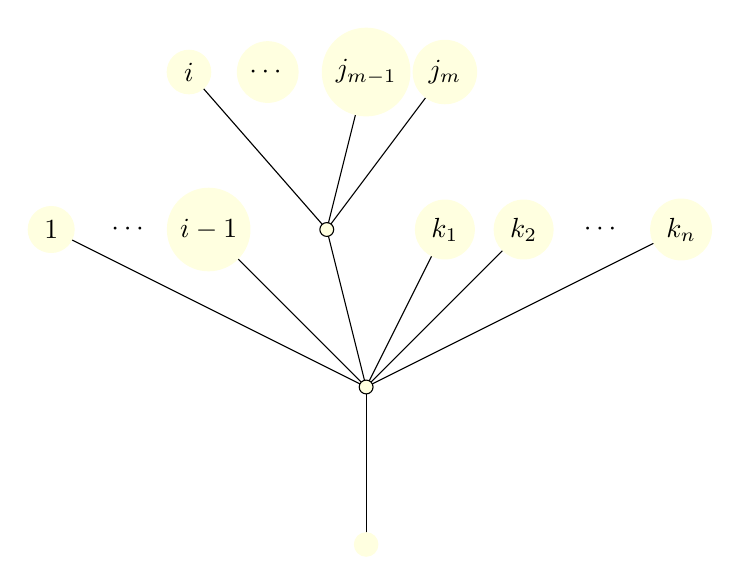
\begin{tikzpicture}
	\begin{pgfonlayer}{main}
		\node [style=inner] (0) at (0, 0) {};
		\node [style=leaf] (1) at (-4, 2) {$1$};
		\node 				(2a) at (-3, 2) {$\cdots$};
		\node [style=leaf] (2) at (-2, 2) {$i-1$};
		\node [style=inner] (3) at (-0.5, 2) {};
		\node [style=leaf] (4) at (-2.25, 4) {$i$};
		\node [style=leaf] (4a) at (-1.25, 4) {$\cdots$};
		\node [style=leaf] (5) at (1, 4) {$j_m$};
		\node [style=leaf] (6) at (0, 4) {$j_{m-1}$};
		\node [style=leaf] (7) at (1, 2) {$k_1$};
		\node [style=leaf] (8) at (2, 2) {$k_2$};
		\node 				(8a) at (3, 2) {$\cdots$};
		\node [style=leaf] (9) at (4, 2) {$k_n$};
		\node [style=leaf] (10) at (0, -2) {};
	\end{pgfonlayer}
	\begin{pgfonlayer}{bg}
		\draw (0.center) to (1.center);
		\draw (2.center) to (0.center);
		\draw (0.center) to (3.center);
		\draw (3.center) to (4.center);
		\draw (3.center) to (6.center);
		\draw (3.center) to (5.center);
		\draw (7.center) to (0.center);
		\draw (0.center) to (8.center);
		\draw (0.center) to (9.center);
		\draw (0.center) to (10.center);
	\end{pgfonlayer}
\end{tikzpicture}

\caption{The two-level trees corresponding
 to partial compositions of shuffle operads}
 \label{fig:twolevel}
\end{figure}
We may as well define the ``total shuffle
composition'' of a tree $T_0$ with trees
$T_1,\ldots,T_n$ along a shuffling partition
$\pi = (\pi_1,\ldots,\pi_n)$ with $T_i$ having
as many leafs as $\pi_i$ for each $i\in \underline{n}$
Concretely, we consider for each such $i$
the unique order preserving bijection
between $\pi_i$ and the labels of $T_i$,
and graft $T_i$ at the input of $T_0$
labelled by $\min \pi_i$. 

\begin{proposition}
The shuffle composition of shuffle tree
monomials is again a shuffle tree
monomial.
\end{proposition} 

\begin{proof}
This is Exercise~\ref{ex:shufflecomp}. The
idea is to note that the local increasing
condition is not broken, and this is clear
on each $T_i$ since we simply relabelled their
leafs with an isomorphic totally order
set, 
while it is not broken on
$T_0$ since we grafted the $T_i$s using
a shuffling partition.
\end{proof}

With this at hand, we can state and prove the
main result in this section. 

\begin{proposition}
The ns collection
$\FF_\XX^\Sha$ with its corresponding
shuffle composition is the \emph{free shuffle
operad} generated by $\XX$, where the
inclusion $\XX\longrightarrow \FF_\XX^\Sha$
sends an element in $\XX$ to the corresponding
corolla with its unique shuffling leaf
labelling. \qed
\end{proposition}

\subsection{Forgetful functor}

Since every finite totally order 
set $I$ is in particular a finite set
$I^{\f}$
after forgetting the order,
we have a functor
$\XX \longmapsto \XX^{\f}$ that assigns
a symmetric collection $\XX$ to the ns
collection $\XX^{\f}$ such that
\[ \XX^{\f}(I) = \XX(I^{\f}) \]
for each finite order set $I$. 
We call this the \emph{forgetful functor}
from symmetric to ns collections. 
The following will be central in what
follows.

\begin{proposition}
The forgetful functor $\SMod \longrightarrow 
\nsMod$ is strong monoidal for the corresponding 
symmetric and shuffle composition products
when restricted
to \emph{reduced} collections, in the sense
that for each pair $\XX$ and $\YY$ with
$\YY$ reduced there is a natural isomorphism
\[
(\XX\circ_\Sigma \YY)^{\f} \longrightarrow
 \XX^{\f}\circ_\Sha \YY^{\f}.
\]
\end{proposition}

\begin{proof}
Let us begin by proving that if $\YY$ is a
reduced symmetric sequence then $\YY^{\otimes n}$
is a free $S_n$-module for every $n\geqslant 1$.
This is of course true for $n=1$. For $n>1$,
it suffices to exhibit an $S_n$-basis. 
For each finite totally ordered set $I$, let
us consider the components of $\YY^{\otimes n}(I^{\f})$,
and note that since $\YY$ is reduced they are of the form
\[
\YY(\pi_1)\otimes \cdots\otimes\YY(\pi_n)
\]
where $\pi$ is a partition of $I$ into $n$ blocks with
at least one element. For each such partition $\pi$
of $I$, there exists a unique permutation $\sigma\in S_n$
such that $(\sigma\pi)_i = \pi_{\sigma^{-1}(i)}$ is
shuffling, and this proves that $\YY^{\otimes n}(I^{\f})$ is
isomorphic to the free $S_n$-module generated
by $(\YY^{\f})^{\otimes_\Sha n}(I)$.
It follows that for each $n\geqslant 1$ we have a
natural isomorphism
\[ 
\XX(n)\otimes_{S_n}\YY^{\otimes n}(I^{\f})
 \longrightarrow 
  \XX^{\f}(n)\otimes (\YY^{\f})^{\otimes_\Sha n}(I)
\] 
which gives us the desired isomorphism
$
(\XX\circ_\Sigma \YY)^{\f} \longrightarrow
 \XX^{\f}\circ_\Sha \YY^{\f}.
$
\end{proof}

\begin{corollary}
For each reduced symmetric collection $\XX$, 
there is a natural isomorphism of shuffle operads
\[
(\FF_\XX^\Sigma)^{\f}
 \longrightarrow \FF_{\XX^{\f}}^\Sha.
\]
Moreover, if $I$ is an ideal in $\FF_\XX^\Sigma$
then $I^\f$ is an ideal in $\FF_{\XX^\f}^\Sha$ and the
resulting quotient shuffle operads are naturally
isomorphic via the induced map
\[
(\FF_\XX^\Sigma/ I )^{\f}
 \longrightarrow \FF_{\XX^{\f}}^\Sha/ I^\f.
\]
\end{corollary}

In particular, shuffle tree monomials on $\XX^{\f}$, when
considered with their non-planar tree structure,
give us a basis of the free symmetric operad on 
$\XX$, and we can study any presentation of a symmetric
operad through the resulting presentation of the
corresponding shuffle operad. 

\subsection{Exercises}

\begin{question}\label{ex:shufflecomp}
 Show that the shuffle composition of shuffle tree
monomials is again a shuffle tree
monomial.
\end{question}
 
\begin{question}
Use the definition of shuffle trees
to compute a basis
of $\mathrm{Tree}_\XX^\Sha(4)$ in case $\XX$ consists
of a single symmetric or antisymmetric
operation. What happens if the operation
is not symmetric?
\end{question}

\begin{question} Explain how 
$\XX^f \circ_\Sha \YY^f$ fails
 to identify with  $(\XX\circ_\Sigma \YY)^f$ 
 in case $\YY$ is
 not reduced. 
\end{question}

\begin{question}
Go through the definition of the shuffle
compositions $\gamma_\pi$ for shuffle
tree monomials, and show that it maps
shuffle tree monomials to shuffle tree
monomials.
\end{question}

\begin{question} 
Give an example of a shuffle operad that
is not obtained from a symmetric operad
through the forgetful functor. \emph{Suggestion:}
ideals coming from symmetric operads must be
stable under the (now non-existent group action).
Can you find a shuffle ideal that is ``not very
symmetric''?
\end{question}

\begin{question}
Write down a presentation of the following as
shuffle operads: the  
commutative operad, the
Lie operad, the
associative operad, and the
operad of $3$-ary totally commutative
associative algebras.
\end{question}

\begin{question}
Repeat the theme of the last four exercises
with any other (quadratic) operad
of your choice.
\end{question}
\newpage

\section{Monomial orders}


\subsection{Some reminders}

In the following, we will anchor ourselves in the 
rewriting theory that exists for associative monoids
in sets and the corresponding theory for
associative algebras. Since we are not assuming
the reader is familiar with this, let us give
a brief recollection of the basics.

\begin{definition}
An associative monoid is a set $M$ along with
an associative multiplication $\mu : M\times M
\longrightarrow M$. Given a set $X$, we write
$\langle X\rangle$ for the free monoid on 
$X$, which is given by the set
$
 \bigsqcup_{n\geqslant 1} X^{n}
 $
of all \emph{words the alphabet $X$} with
product the isomorphism
$ X^n\times X^m \cong X^{m+n}$
for each $m,n\geqslant 1$.
\end{definition}

We are interested in finding bases of 
free objects by ideals and, to do this,
we will resort to ordering our free objects.
This will allow us to give a (terminating)
algorithm whose input will be a set of 
relations and an ordering, and whose
output (among other things) will 
be a basis of our quotient object.

\begin{definition}

An ordered monoid is a pair $(M,\prec)$ where $M$ is a monoid
and $\prec$ is a total order on $M$ that satisfies the
following three conditions:
\begin{tenumerate}
\item It is a well-order: every non-empty subset of $M$
has a minimum. 
\item The product map of $M$ is increasing in both of its
arguments for $\prec$. 
\end{tenumerate}
A \emph{monomial order} on the alphabet $X$ is, by definition,
the structure of an ordered monoid on the free monoid $\langle X\rangle$
generated by $X$.
\end{definition}

Explicitly, the last condition requires that if $m_1,m_2,m_3\in M$
and if $m_1\prec m_2$ then it follows that $m_3m_1\prec m_3m_2$ 
and $m_1m_3\prec m_2m_3$. If the alphabet $X$ is given a total order, 
then we can produce a monomial order on it as follows:

\begin{definition}
Let $\prec$ be a total order on $X$. 
The graded lexicographic order on $\langle X\rangle$
induced by $\prec$, which we write $\prec_\ell$,
is such that $w\prec_\ell w'$ if and only if
\begin{tenumerate}
\item The word $w$ is shorter than $w'$, or else
\item We have
$w = w_1 xw_2$ and $w' = w_1 y w_2'$ with
$x\prec y$ in $X$.
\end{tenumerate}
\end{definition}

It is important to note that the lexicographic order defined only
by the second condition is \emph{not} a well-order, and it is 
not increasing for the concatenation product: for example,
if $x\prec y$ then $x \prec x^2$ but $x^2y \prec xy$. 

\begin{lemma}
The graded lexicographic order is a monomial order on $X$
for any choice total order $\prec$.
\end{lemma}

\begin{proof}
It is clear that the resulting order is total, for either
two words are of distinct length, or they are of the same length
and differ at and entry, or else they are equal. To see the
order behaves well with respect to the concatenation product,
we observe that the function $w\longmapsto \mathrm{Length}(m)$
is additive for the concatenation product, so if $w$ is longer
than $w'$, then $ww''$ will be longer than $w'w''$ and,
similarly, $w''w$ will be longer than $w''w'$. If $w$ and 
$w'$ have the same length, then it is clear that
$w''w'\prec w''w$ if and only if $w'w''\prec ww''$ if
and only if $w' \prec w$. To see that the order is a well
order, let us consider a collection $W$ of words. Then,
in particular, there exists a least natural number $n$
such that $W$ contains words of length $n$ but not of $n-1$. 
In this case, it follows that the minimum of $W$, if it
exists, must be contained in the set $X^n$, and this
set is well ordered by the lexicographical order if
$X$ it itself well ordered: we can find the minimum 
by induction on $n$.
\end{proof}

We now recall Lecture~\ref{lecture:thebasics} the 
definition
of the \emph{word operad of a monoid $M$},
which appeared recently in~\cite{Dotsenko2020}.


\begin{definition}
Let $M$ be an associative monoid. The symmetric
operad $\mathbb W_M$ is defined by $\mathbb{W}_M(n) =
M^n$ for each $n\geqslant 1$, and its partial composition
product is defined for each $s,t\geqslant 1$ and each
$i\in [s]$ by the rule
\[(m_1,\ldots,m_s) \circ_i (m_1',\ldots,m_t') = 
 	(m_1,\ldots,m_{i-1}, m_im_1',\ldots,m_im_t',m_{i+1},\ldots, m_s).\] 
\end{definition}

The reader should verify that $\mathbb W_M$ is isomorphic,
as a symmetric sequence, to the composition product $\mathrm{Ass}\circ M$,
where we consider $M$ a symmetric sequence concentrated in arity $1$. 

\subsection{Two statistics}

Of particular interest to us is the case $\XX$ is
a reduced symmetric sequence in sets, and we let
$\underline{\XX} = \bigsqcup_{n\geqslant 1} \XX(n)$
be the underlying alphabet of $\XX$. We will use
the notation $\XX^*$ for the free monoid $\langle 
\underline{\XX}\rangle$. By definition, there
exists a unique map of shuffle operads
$
\pi : \FF_\XX^\Sha \longrightarrow
						\mathbb W_{\XX^*} 				
$ 
extending the map $\XX \longrightarrow \mathbb W_{\XX^*}$
that assigns $x\in \XX(n)$ to the element
$(x,\ldots,x)\in \mathbb W_{\XX^*}(n)$.

\begin{definition}
For each shuffle tree monomial $T$, we call 
$\pi(T)$ the \emph{path sequence of $T$.}
\end{definition}

The path sequence of a shuffle tree monomial $T$ can
be computed in a straight-forward way, as the following
lemma shows. The useful observation that the previous
definition allows us to make is that the path
sequence statistic is compatible with shuffle 
compositions of tree monomials, in the sense the
path sequence of a composition of tree 
monomials equals the compositions
of the corresponding path sequences of these
tree monomials.
 
\begin{figure}[h]
\[ 
	\leftc{x}{y}{1}{2}{3}
 \quad
		\leftc{x}{y}{1}{3}{2} 
		\qquad
		\rightc{y}{x}{1}{2}{3}
		\]
		\[ \hspace{0.4 in}(yx,yx,y)
			\hspace{.8 in} (yx,y,yx)
				\hspace{0.8 in}(y,yx,yx)\]
		\caption{An example of the computation of path sequences.}
		\label{fig:paths}
		\end{figure}
		
\begin{lemma}
Let $\XX$ be reduced. 
The path sequence of $T$ is the tuple in $\mathbb{W}_{\XX^*}(n)$
where $n$ is the number of leaves of $T$, obtained by recording at the
$i$th entry the word in $\XX$ read by travelling from the root of
$T$ to the leaf labelled by $i$.
\end{lemma}

More generally, in case $\XX$ has $0$-ary variables, we must look at 
all \emph{endpoints} of a tree monomial. Since we will not be
interested in non-reduced alphabets, we let the curious reader
explore this modification on their own. It is useful to remark
in situations like this that $\underline{\XX}$ is obtained 
through a disjoint union of the components
of $\XX$: the path sequence of $x\circ_1 y$ for $x$ and $y$ unary
is $(xy)$, and the path sequence of $x\circ_1 y'$ for $x$ unary and
$y'$ nullary is `also' $(xy')$, but these are \emph{distinct}
in the free monoid $\XX^*$. 

\begin{proof}
This is Exercise~\ref{ex:pathseq}.
\end{proof}

Let us now consider the unique  map of shuffle operads
$\sigma : \FF_\XX^\Sha \longrightarrow
						\mathsf{Ass}$ 
extending the map $\XX \longrightarrow \mathsf{Ass}$
that assigns $x\in \XX(n)$ to the identity
$1\in \mathsf{Ass}(n) = S_n$. 

\begin{definition}
If $T$ is a shuffle tree monomial. 
we call $\sigma(T)$ the (leaf) permutation sequence of $T$.
We call the pair $(\pi(T),\sigma(T))$ the
path-permutation data of $T$. 
\end{definition}

As before, this statistic of $T$ has a simpler description,
that can be read off directly from $T$, and the previous
definition tells us that the leaf permutation
sequence of a tree monomial behaves well with
respect to shuffle compositions.

\begin{figure}
\[
\fork{x}{y}{x}{1}{3}{2}{4}
\qquad
\fork{x}{y}{x}{1}{4}{2}{3}
\qquad
\fork{x}{y}{x}{1}{2}{3}{4}
\]
\caption{Three different shuffle three monomials with the same path
sequence, but different permutation sequence.}
\end{figure}

\begin{lemma}
The permutation sequence of $T$
 is obtained by reading the leaf labelling of $T$ from
left to right and recording it as a permutation in
``two line notation''.
\end{lemma}

The main result of this section tells us that it suffices
for us to order sequences of words in the alphabet $\XX$
and permutations in order to order shuffle tree monomials.

\begin{theorem}
The map $\FF_\XX^\Sha \longrightarrow \mathbb{W}_{\XX^*}\times
\mathsf{Ass}$ of the free shuffle operad on $\XX$ into the 
Hadamard product of $\mathbb{W}_{\XX^*}$ and $\mathsf{Ass}$
induced by $\pi$ and $\sigma$ is injective.
In other words, the path-permutation datum of a shuffle
tree monomial determines it uniquely.
\end{theorem}

Let us call the map in the statement of the theorem the
\emph{path-permutation inclusion}.

\begin{proof}
We will sketch a proof, and ask the reader to fill in the
details as an exercise; we proceed by induction on the
total length of the path sequence of a tree monomial so that,
for example, the path sequences appearing in Figure~\ref{fig:paths}
have all length five. First, let us show that the path sequence
determines the planar structure of our tree monomial uniquely:

If the length is zero, then the path sequence $\pi$
is empty, and we are simply considering the trivial tree monomial.
Let us consider now some positive length $\ell$ and search,
among all words $w$ appearing in $\pi$, that which has
the largest possible length and smallest possible coordinate,
let us say this coordinate is $i$.

If $w$ ends in a $0$-ary variable of $\XX$, this means the
$i$th leaf of $T$ ends at a stump, and we can remove it, 
and continue by induction. If not, then $w$ ends with
some variable $x\in \XX(k)$, and the way we have chosen
it implies that the $i$th leaf (in the planar order)
is the first child of $x$, and that all other children
of $x$ are also leaves. It follows that $w$
and the next $k-1$ words in $\pi$ all end with $x$,
and that $\pi$ is obtained as a non-symmetric composition
with $(x,\ldots,x)$. By pruning $x$ from $\pi$, we
can proceed by induction. 

Now that we know the path sequence recovers the planar structure
of $T$ uniquely, let us pick some path-permutation datum
$(\pi,\sigma)$. Then, reorder the entries of $\pi$ using
$\sigma^{-1}$ to recover the planar structure of $T$,
and then label its leafs according to $\sigma$, to 
recover the whole shuffle structure.
\end{proof}


\subsection{Ordered shuffle operads}

We can now proceed to define ordered shuffle operads. 

\begin{definition}
A set shuffle operad $\PP$ is order if for each $n\geqslant 0$
the component $\PP(n)$ is well-ordered and if shuffle compositions
are increasing in each of its arguments: for each $n\geqslant 1$,
all elements $(T_0;T_1,\ldots,T_n) \in\PP(k)\times \PP(n_1)
\times \cdots\times \PP(n_k)$ and all shuffling partitions
of $\underline{n}$ for $n=n_1+\cdots +n_k$, we have that
\[ 
\gamma_\pi(T_0;T_1,\ldots,T_i, \ldots, T_n)  \prec
\gamma_\pi(T_0;T_1,\ldots,T_i',\ldots,T_n)
\]
whenever $T_i\prec T_i'$  for some $i\in [0,n]$ as elements
of $\PP(n_1+\cdots+ n_k)$. 
\end{definition}

In particular, we can apply this definition in the case $\PP$
is the free shuffle set operad on some alphabet $\XX$. As
promised, let use 
the injection $(\pi,\sigma)$ to endow tree monomials with
well-orders. 

\begin{proposition}[Proposition 1.6 in ~\cite{Dotsenko2020}]
Let $(M,\prec)$ be an ordered monoid. The
word operad on $\mathbb W_M$ is an ordered operad
through the lexicographical order of words.
\end{proposition}

\begin{proof}
This is Exercise~\ref{ex:orderedM}.
\end{proof}

In particular, we can consider the case in which $M = \XX^*$
is endowed with the graded lexicographical order induced by
a total order on $\underline{\XX}$, which implies the following
corollary.

\begin{corollary}
Suppose that $\underline{\XX}$ is given a total order, and that
we give the free monoid $\XX^*$ the induced graded 
lexicographical order. Then
the word operad $\mathbb{W}_{\XX^*}$ is an ordered
shuffle operad with the lexicographical order.
\end{corollary}

We leave it as an exercise to the reader to show that the
associative operad is an ordered shuffle operad if we
use on it the lexicographic order on permutations
(seen as strings of numbers, in one line notation).
All our work is now, done:

\begin{definition}
Let $\XX$ be an alphabet and suppose that we
give the monoid $\XX^*$ a monomial order $\prec$.
The \emph{path-permutation extension} of $\prec$ is the
unique order on $\FF_{\XX}^\Sha$ induced by
the path-permutation inclusion, where we use the
the induced lexicographic
order on $\mathbb{W}_{\XX^*}$ first, and the
lexicographic order on $\mathsf{Ass}$ second.
\end{definition}

Naturally, one can switch the roles of the two
factors of the path-permutation inclusion to get
the \emph{permutation-path extension} of a monomial
order on $\XX^*$. We will explore other variations
in the exercises.

\begin{definition}
Let us fix a total order $\prec$ on $\underline{\XX}$, and let us
consider the induced graded lexicographic order on 
$\XX^*$, where we first compare the length of a 
word, and then use the lexicographic order induced
by the total order. The path-permutation extension 
on $\FF_\XX^\Sha$ is called the  \emph{graded path-permutation 
lexicographic order} induced by $\prec$.
\end{definition}

For example, let us consider the case in which $\XX$ is binary
and contains exactly two operations $x$ and $y$. The next
figure shows the \texttt{grapathpermlex} order induced by $x<y$
on all possible twelve tree monomials with three leaves on $\XX$;
largest elements appear first, from top left to bottom right.

\[ 
	\leftc{y}{y}{1}{2}{3}
 \quad
		\leftc{y}{y}{1}{3}{2}
		\qquad
			\leftc{x}{y}{1}{3}{2} 
		\]
		\[ \hspace{0.4 in}(yy,y,y)
			\hspace{.8 in}(yy,y,yy) \hspace{0.8 in}
			(yx,yx,x)
				\]
		
\[ 
\leftc{x}{y}{1}{3}{2}
 \quad
			\leftc{y}{x}{1}{2}{3}
		\qquad
	\leftc{y}{x}{1}{3}{2} 
		\]
		\[ \hspace{0.4 in}(yx,x,yx)
			\hspace{.8 in} (xy,xy,x)
				\hspace{0.8 in}(xy,x,xy)\]
		
\[ 
\leftc{x}{x}{1}{2}{3} \quad
\leftc{x}{x}{1}{3}{2} 	\qquad
\rightc{y}{y}{1}{2}{3}
		\]
\[ \hspace{0.4 in}(xx,xx,x)
			\hspace{.8 in} (xx,x,xx)
				\hspace{0.8 in}(y,yy,yy)\]

\[ 
\rightc{y}{x}{1}{2}{3} \quad
\rightc{x}{y}{1}{2}{3}		\qquad
\rightc{x}{x}{1}{2}{3}
		\]
		\[ \hspace{0.4 in}(y,yx,yx)
			\hspace{.8 in} (x,xy,xy)
				\hspace{0.8 in}(x,xx,xx)\]
		
		



\newpage

\subsection{Exercises}
 
\begin{question}\label{ex:pathseq}
Show that the path sequence of a tree monomial, as defined
using the universal property of the free shuffle operad,
coincides with its combinatorial definition obtained
by reading the entries of the tree from the
root to the leaves.
\end{question}
 
\begin{question}
Let $X$ be a finite set and let us give 
$\langle X\rangle$ the graded lexicographical order with
respect to a fixed total order on $X$. Show this is a
monomial order.
\end{question}

\begin{question}\label{ex:orderedM}
Suppose $(M,\prec)$ is an ordered monoid and
we let us give the shuffle operad
$\mathbb{W}_M$ the induced lexicographical 
order. Show that the resulting order is a monomial
order.
\end{question}

\begin{question}
Consider the ns collection $\XX$ with $\underline{\XX} = \XX(2)$
a singleton. Show that we can always find a monomial order that
singles out one of the three shuffle tree monomial basis
elements of $\FF_\XX^\Sha(3)$ as the largest. 
\end{question}

\begin{question}
Consider the ns collection $\XX$ with $\underline{\XX} = \XX(2)
= \{x,y\}$, and the ``mixed'' shuffle tree monomials in 
$\FF_\XX^\Sha(3)$ that have $x$ and $y$ (one at the top,
the other at the bottom). Explore what leading terms
you can obtain by choosing different induced orders
on $\FF_\XX^\Sha$.
\end{question}
\afterpage{\blankpage}
\newpage
 

\section{Gr\"obner bases}\label{lecture:GB1}

\textbf{Goal.} Define the long division algorithm for shuffle
tree polynomials. Prove Gr\"obner bases for shuffle operads exist
and reduced Gr\"obner bases are unique.

\subsection{Tree insertion}

\begin{definition}
Let $T'$ and $T$ be tree monomials over some fixed alphabet $\XX$.\
We say that $T'$ divides $T$ if the underlying tree $\tau$
of $T$ contains a subtree $\tau_0$ isomorphic to the underlying
tree $\tau'$ of $T'$, whose induced shuffling labelling
 and decorations coincide with that of $T'$.
 \end{definition}
\begin{figure}[h]
\[
\fork{x}{y}{x}{1}{3}{2}{4}
\mathsymbol{1.5}{\text{is divisible by}}
\begin{tikzpicture}[scale = .75]
\tikzstyle{inner}=[circle,draw=black, fill=white, inner sep=1pt,minimum size=5pt]
\tikzstyle{leaf}=[circle, draw=white, fill=white, inner sep=3 pt,minimum size=5 pt]
	\begin{pgfonlayer}{main}
		\node [style=inner] (0) at (0, 0) {$x$};
		\node [style=inner] (2) at (-1, 1) {$x$};
		\node [style=leaf] (9) at (1, 1) {$2$};
		\node [style=leaf] (10) at (0, -1.25) {};
		\node [style=leaf] (11) at (-1.5, 2) {$1$};
		\node [style=leaf] (12) at (-0.5, 2) {$3$};
	\end{pgfonlayer}
	\begin{pgfonlayer}{bg}
		\draw (2.center) to (0.center);
		\draw (0.center) to (9.center);
		\draw (0.center) to (10.center);
		\draw (2.center) to (11.center);
		\draw (12.center) to (2.center);
	\end{pgfonlayer}
\end{tikzpicture}
\mathsymbol{1.5}{\text{and by}}
\begin{tikzpicture}[scale = .75]
\tikzstyle{inner}=[circle,draw=black, fill=white, inner sep=1pt,minimum size=5pt]
\tikzstyle{leaf}=[circle, draw=white, fill=white, inner sep=3 pt,minimum size=5 pt]
	\begin{pgfonlayer}{main}
		\node [style=inner] (0) at (0, 0) {$x$};
		\node [style=leaf] (2) at (-1, 1) {$1$};
		\node [style=inner] (9) at (1, 1) {$y$};
		\node [style=leaf] (10) at (0, -1.25) {};
		\node [style=leaf] (13) at (0.5, 2) {$2$};
		\node [style=leaf] (14) at (1.5, 2) {$3$};
	\end{pgfonlayer}
	\begin{pgfonlayer}{bg}
		\draw (2.center) to (0.center);
		\draw (0.center) to (9.center);
		\draw (0.center) to (10.center);
		\draw (13.center) to (9.center);
		\draw (9.center) to (14.center);
	\end{pgfonlayer}
\end{tikzpicture}
\]
\caption{A ``fork'' and its divisors of weight two. Notice the induced labelling of the right comb, coming from the
shuffling labelling $1<2<4$.}
\end{figure}

The following lemma asserts that the combinatorial notion
of divisibility coincides with the algebraically inclined
notion of divisibility, that of belonging to the ideal
generated by the divisor. 

\begin{lemma}
A tree monomial $T$ is divisible by another
tree monomial $T'$ if and only if it can be obtained
from $T'$ by iterated shuffle compositions with
other tree monomials.
\end{lemma}

\begin{proof}
It is clear that if $T$ is obtained from $T'$ by
iterated shuffle compositions with tree monomials,
then $T$ is divisible by $T'$. Conversely, suppose
$T'$ divides $T$. If the root of $T'$ is not that of
$T$, then we can write $T$ as a composition of several
tree monomials, one which is divisible by $T'$ and
which shares the root with it, so we may assume this is
the case. One this is done, we see that $T$ is in fact
obtained by grafting tree monomials at the leaves of $T'$,
and completes the proof.
\end{proof}

\begin{figure}[t]

\[
\Leftc{x}{y}{x}{1}{3}{2}{4}
\mathsymbol{1.5}{\text{is divisible by}}
\leftc{x}{y}{1}{3}{2}
\mathsymbol{1.5}{\text{and by}}
\leftc{y}{x}{1}{2}{3}
\]
\caption{A right comb with two divisors that have
the same underlying planar structure but different
induced labelling.}
\end{figure}
\begin{definition}
Suppose that $T'$ is a divisor of $T$, and let us
assume that $T'$ has $\ell'$ leaves and $T$
has $\ell$ leaves. We define the insertion operation
\[
\repl{T'}{T}{-}: \FF_\XX^\Sha(\ell') \longrightarrow 	
 \FF_\XX^\Sha(\ell) 
\]
that replaces the divisor $T'$ of $T$ by any other
shuffle tree monomial with $\ell'$ leaves
in $T$, and extend it linearly, making sure
that leaf labels are respected.
\end{definition}
\begin{figure}[b]
\[
\Leftc{x}{x}{x}{1}{2}{3}{4}
\mathsymbol{1.5}{\text{ is divisible ``twice'' by}}
\leftc{x}{x}{1}{2}{3}
\]
\caption{A right comb with two divisors that have the
same induced shuffle tree structure, but happen
at different places of the tree.}
\end{figure}
\begin{lemma}
Let $\mathcal{V}$ be a subset of the free shuffle operad on $\XX$.
Then the ideal generated by $\mathcal{V}$ is explicitly obtained
as the linear span of all insertions $\repl{T'}{T}{f}$
as $T,T'$ range through pairs $(T',T)$ with $T'$ a divisor
of $T$ and $f\in \mathcal V(\ell')$.
\end{lemma}

\begin{figure}[h]
\[
\begin{tikzcd}
{} &\phantom{\hspace{-3.5 em}}\Leftc{x}{x}{x}{}{}{}{} 
	\arrow[dr] 
	\arrow[dl] \\
\fork{x}{x}{x}{}{}{}{}&  {} & \Leftr{x}{x}{x}{}{}{}{}
\end{tikzcd}
\]
\caption{Two possible results of substituting
a left comb by a right comb in the leftmost tree.}
\end{figure}

\begin{proof}
By construction, $(\mathcal V)$ is the linear span of all possible
shuffle compositions where at least one summand is contained in
$\mathcal V$. Since shuffle compositions are multilinear, we can
assume that all terms appearing in such shuffle compositions (except,
possibly, for that in~$\mathcal V$) are tree monomials, in which case
the resulting shuffle composition coincides with an insertion
operation.
\end{proof}

\subsection{Long division}

Suppose that we fix a tree monomial order on the free
shuffle operad $\FF_\XX^\Sha$ and $f \in \FF_\XX^\Sha(n)$
is a tree \emph{polynomial}. The support of $f$ is the (finite)
set of tree monomials that appear in $f$ with non-zero coefficient.
We say the tree monomial $T$ is
the \emph{leading monomial of $f$} if $T$ is the largest monomial
that appears in the support of $f$, and we write the corresponding
summand in $f$ by $\leadm{f}$. This summand is accompanied by a
coefficient, which we call the leading coefficient of $f$ and
write $\leadc{f}$. Thus, any $f$ can be written in the form
\[ f = \leadc{f} \leadm{f} + f_0 \]
where all monomials appearing in $f_0$ are smaller than $\leadm{f}$.
We call $\leadc{f} \leadm{f}$ the leading term of $f$ and write
it $\lead{f}$. We begin with a preparatory result.

\begin{figure}[h]
\[ 
	\mathsymbol{1.5}{f_1 =}	\underline{\leftc{x}{y}{1}{2}{3}}
\mathsymbol{1.5}{+}		\leftc{x}{y}{1}{3}{2} 
		\mathsymbol{1.5}{+}	
		\rightc{y}{x}{1}{2}{3}
		\]
		\[ 
	\mathsymbol{1.5}{f_2 =}	\leftc{x}{x}{1}{2}{3}
\mathsymbol{1.5}{-}	\underline{\leftc{x}{y}{1}{3}{2} }
		\]
		\[ 
	\mathsymbol{1.5}{f_3 =}	 \underline{\leftc{x}{y}{1}{2}{3}}
		\mathsymbol{1.5}{-}	
	\rightc{x}{x}{1}{2}{3} \mathsymbol{1.5}{+}	 \rightc{y}{y}{1}{2}{3}
		\]
		\caption{Leading terms underlined in some tree polynomials, for
		the \texttt{grpathpermlex} order induced by $y>x$.}
		\label{fig:orders}
		\end{figure}
		
		
\begin{proposition}\label{prop:repllead}
Suppose that $T'$ is a divisor of $T$ and let $f\in \FF_\XX^\Sha(\ell')$.
Then the leading term of the insertion $\repl{T'}{T}{f} = \square_{T'}^T(f)$
is equal to $\repl{T'}{T}{\lead{f}}$.
\end{proposition}

\begin{proof}
For tree polynomials $f_0,f_1,\ldots,
f_n$ and any shuffling partition $\pi$, we have that
\[ \lead{\gamma_\pi(f_0;f_1,\ldots,f_n) }= 
 		\gamma_\pi(\lead{f_0};\lead{f_1},\ldots,\lead{f_n}).
 		\]
This is clear, since the shuffling compositions are by definition
(strictly) increasing for $\prec$. Since we know that $\repl{T'}{T}{f}$
is obtained from $f$ be iterating shuffle compositions, this proves
the statement of the proposition. 
\end{proof}

Let $\mathcal{V}$ be a subset of the free shuffle operad on $\XX$. A
tree monomial $T$ is reduced with respect to $\mathcal{V}$ if it is
not divisible by any of the leading terms of polynomials appearing in it.
A polynomial is reduced with respect to $\mathcal V$ if it is a linear
combination of tree monomials that are reduced. We say $\mathcal V$
is self-reduced if each $v\in \mathcal V$ is reduced with respect to
$\mathcal V\smallsetminus v$, and that is is linearly self-reduced
if no leading term of one element divides the leading term of 
another. 

\begin{definition}[Reduction]\label{def:reduce}
Suppose that $f$ and $g$ are polynomials of the same arity, and
that $f$ is divisible by the leading term of $g$, in other words,
suppose that $\lead{f} = \repl{T'}{T}{\lead{g}}$ for some
tree monomial $T$ and a divisor $T'$. In this case,
the reduction of $f$ with respect to $g$, which we write
$r_g(f)$, is defined by
\[
r_g(f) = f - \frac{\leadc{f}}{\leadc{g}} \repl{T'}{T}{g}.
\]
\end{definition}

The following lemma tells us that the reduced term $r_g(f)$ 
behaves like a ``remainder by division'', in the sense it is
either zero of ``smaller than $f$''.

\begin{lemma}\label{lemma:smaller}
For all $f$ and $g$ such that $r_g(f)$ is defined, either
$r_g(f)= 0$, or else we have that $\lead{r_g(f)} \prec \lead{f}$.
\end{lemma}

\begin{proof}
If $r_g(f)$ is non-zero, we have that its leading coefficient is 
equal to the leading coefficient of $f- \frac{\leadc{f}}{\leadc{g}}\repl{T'}{T}{g}$. But the leading term of the second term is, by
Proposition~\ref{prop:repllead}, equal to 
\[ \frac{\leadc{f}}{\leadc{g}}\repl{T'}{T}{\lead{g}} =  \leadc{f} \leadm{f} 
	= \lead{f}.\]
It follows that the terms appearing in $r_g(f)$ are all strictly smaller
than the leading term of $f$, as we wanted. 
\end{proof}

\textbf{Long division algorithm.}
Let us now define the long division algorithm for shuffle operads.
Its input is a polynomial $f$ and a finite set $\mathcal V$, both
in $\FF_\XX$, and its
output is a reduced element $\overline{f}$ with respect to $\mathcal
V$ such that $f-\overline{f} \in (\mathcal V)$ and $\lead{\overline{f}}
\preceq \lead{f}$. We can verbosely describe the algorithm as follows: 
\begin{tenumerate}
\item If our input polynomial
$f$ is zero, just return zero. If not, ensure $\mathcal V$
is linearly self-reduced, using the linear self-reduction
Algorithm~\ref{algo:gauss}.
\item If there is an element $v$ in $\mathcal V$ 
whose leading term divides the
leading term of $f$, pick that with the largest leading term.\footnote{This
 can be done since we already ensured $\mathcal V$ is linearly
self reduced.}
\item Let $f'$ be the remainder of division of $f$
by $v$ using the reduction procedure of Definition~\ref{def:reduce}.
Recursively call the algorithm to compute the result of long
division of $f'$ by $V$.
\item If not, then $\lead{f}$ is $\mathcal V$-reduced, 
so let $f'$ be the result of long division of $f-\lead{f}$ by $\mathcal V$, and return $\lead{f} + f'$.
\end{tenumerate}
The following is what this algorithm looks like in pseudo-code:
\begin{algorithm}
\caption{Long division algorithm}\label{euclid}
\textsc{Input:} A polynomial $f$ and a finite set $\mathcal V$
of tree polynomials.

\textsc{Output:} A $\mathcal V$-reduced polynomial $\overline{f}$ with $f-\overline{f} \in (\mathcal V)$ and $\lead{\overline{f}}
\preceq \lead{f}$.
\begin{adjustwidth}{1 cm}{1 cm}
\begin{algorithmic}[1]
\Procedure{LongDivision}{\texttt{TreePolynomial},\texttt{TreePolynomials}}
\If {$\texttt{TreePolynomial}=0$} \Return $0$
	 \Else
	 \State $\texttt{Dividend} \gets \texttt{TreePolynomial}$
	 \State $\texttt{Divisors} \gets 
	 	\textsc{LinearSelfReduce}(\texttt{TreePolynomials})$
	 \State $\texttt{Factors} \gets \{ v\in \texttt{Divisors} :\leadm{v} \text{ divides } \lead{g}\}$
	\If {$\texttt{Factors} \neq \varnothing$}
	\State $\texttt{LargestFactor}\gets \textsc{Largest}(\texttt{Factors})$   
	\State $\texttt{Dividend}\gets \textsc{Reduce}(\texttt{Dividend},\texttt{LargestFactor})$ 
	\State $\texttt{Dividend}\gets \textsc{LongDivision}(\texttt{Dividend},\texttt{Divisors})$  
		\EndIf
	\State $\texttt{LeadDividend} \gets \lead{\texttt{Dividend}}$
	\State $\texttt{Dividend} \gets \texttt{Dividend}-\texttt{LeadDividend}$
	\State $\texttt{Dividend} \gets \textsc{LongDivison}(\texttt{Dividend},\texttt{Divisors})$
	\EndIf
	\State \Return $\texttt{LeadDividend} + \texttt{Dividend}$
\EndProcedure
\end{algorithmic}
\end{adjustwidth}
\end{algorithm}


\begin{lemma}
The long division algorithm terminates, and its
output is a reduced element $\overline{f}$ with respect to $\mathcal
V$ such that $f-\overline{f} \in (\mathcal V)$ and $\lead{\overline{f}}
\preceq \lead{f}$.
\end{lemma}


\begin{proof}
At each step, the leading monomial of $f$ is decreased Lemma~\ref{lemma:smaller},
so the fact that $\prec$ is a well order guarantees our algorithm
terminates. It also guarantees that the output will satisfy
$\lead{\overline{f}} \preceq \lead{f}$. Let us suppose, for the sake
of a contradiction, that the output of the algorithm is not
always reduced. Among such problematic polynomials $f$,
let us pick one $f$ with the smallest leading term, which is
possible since $\prec$ is a well order. If $\lead{f}$ is not
reduced, then the first step of our algorithm applies long
division to $r_g(f) = f'$ for some $g\in\mathcal V$, and
by Lemma~\ref{lemma:smaller}, this is either zero or has a smaller
leading term than $f'$, so it must be reduced. If $\lead{f}$
is reduced, then the second step of the algorithm applies long
division to $f-\lead{f}$, which has smaller leading term than
$f$, so the output is again reduced. Finally, note that
at each step of the algorithm we subtract an element of
$\mathcal V$, so the coset of $f$ is not modified,
which concludes our proof.
\end{proof}

\begin{proposition}
Suppose that $\mathcal I$ is an ideal in the free shuffle
operad generated by $\XX$. Then those shuffle monomials that
are reduced with respect to $\mathcal I$ form a basis
for the quotient operad $\FF_\XX / \mathcal I$.  
\end{proposition}

\begin{proof}
Let us first show that these monomials span the quotient operad.
This follows, for the long division algorithm guarantees
we can always replace a non-reduced polynomial $f$ by a reduced
one without affecting its coset. To see they are linearly
independent, suppose that $f$ is a polynomial reduced with
respect to $I$, and that $f\in \mathcal I$. Then we see that
$\lead{f} \in \lead{\mathcal I}$. But this can only happen if
$f=0$ (or else $f$ would not even be linearly reduced with respect
to $\mathcal I$). 
\end{proof}

In practice, we
have little control over the multitude of leading terms
that may appear in the elements of $\mathcal I$,
and Gr\"obner bases are designed to regain this control. 
 
 \bigskip
 
 \textbf{Self-reduction algorithm.} Suppose that
 $\mathcal V$ is a finite subset of $\FF_\XX^\Sha$. 
 The following
 algorithm takes as input this generating set,
 and outputs a self-reduced subset $\mathcal V'$
 that generates the same ideal as $\mathcal V$. 
 This is what this algorithm looks like in pseudo-code, 
 though we are being slightly imprecise: $\mathcal V$ is
 not a matrix, so we cannot feed it to our linear self
 reduction algorithm as is: we pick a total order on
 $\mathcal V$, and then use the corresponding matrix
 written in the shuffle tree monomial basis. 
 
 \begin{algorithm}
\caption{Self-reduction algorithm}\label{algo:self-reduce}
\textsc{Input:} A finite set of polynomials $\mathcal V$ in a
free shuffle operad.

\textsc{Output:} A finite self-reduced set of polynomials 
generating the same ideal as $\mathcal V$.
\begin{adjustwidth}{1 cm}{2 cm}
\begin{algorithmic}[1]
\Procedure{SelfReduce}{$\texttt{Polynomials}$}
	\State $\texttt{ToReduce} \gets \textsc{LinearSelfReduce}(\texttt{Polynomials})$
\If {$\texttt{ToReduce}$ is self reduced} \Return $\texttt{ToReduce}$
\Else 
\State $\texttt{Largest} 
	\gets \textsc{Largest}(\texttt{ToReduce})$
\State $\texttt{ToReduce} \gets \textsc{SelfReduce}(\texttt{ToReduce}\smallsetminus \texttt{Largest} )$
\State $\texttt{NewElement} \gets \textsc{LongDivision}(\texttt{Largest} ,\texttt{ToReduce})$
\State $\texttt{ToReduce}\gets \texttt{ToReduce}\cup \texttt{NewElemet}$
\EndIf
\State \Return $\textsc{SelfReduce}(\texttt{ToReduce})$
\EndProcedure
\end{algorithmic}
\end{adjustwidth}

\end{algorithm}

 \begin{proposition}\label{lemma:self-reduction}
 The self-reduction algorithm terminates for each
 finite set $\mathcal V$ and returns a self-reduced
 set $\mathcal V'$ with $(\mathcal V) = (\mathcal V')$.
\end{proposition}  

\begin{proof}
This is Exercise~\ref{ex:self-reduction}.
\end{proof}
\subsection{Existence and uniqueness}

\begin{lemma}
Let $\mathcal I$ be an ideal of $\FF_\XX$. The subspace 
\[
\lead{\mathcal I} = \langle T \in \FF_\XX : \text{ $T = 
	\lead{f}$ for some  $f\in\mathcal I$} \rangle.
\]
spanned by leading terms of elements of $\mathcal I$ is
again an ideal of $\FF_\XX$.
\end{lemma}

\begin{proof}
By construction $\lead{\mathcal I}$ is a subspace of $\FF_\XX$, so 
it suffices we prove it is an ideal. By multilinearity, it suffices
to show it is stable under compositions with respect to tree
monomials if at least one term is already in $\lead{\mathcal I}$.
To do this, note that if
$T$ is the leading term of some $f\in\mathcal I$, then by
Proposition~\ref{prop:repllead}, for any tree monomials
$T_0,\ldots,T_{i-1},T_{i+1},\ldots,T_n$, the leading term
of the composition 
\[ \gamma_\pi(T_0;T_1,\ldots,T_{i-1},f,T_{i+1},\ldots,T_n)\in \mathcal I\]
is precisely $\gamma_\pi(T_0;T_1,\ldots,T_{i-1},T,T_{i+1},\ldots,T_n)$,
which proves this belongs to $\lead{\mathcal I}$.
\end{proof}

\begin{definition}
Let $\mathcal I$ be an ideal of $\FF_\XX$. We say that a subset
$\mathcal G$ of $\mathcal I$ is a \emph{Gr\"obner basis of $\mathcal I$}
(with respect to our fixed monomial order) if the set of leading monomials
of $\mathcal G$ generate the ideal of leading terms of $\mathcal I$.
A Gr\"obner basis which is self-reduced is called reduced.
\end{definition}

\begin{lemma}
Let $\mathcal I$ be an ideal and let $\mathcal G$ be a 
Gr\"obner basis of $\mathcal I$. Then $\mathcal G$ 
generates $\mathcal I$.  
\end{lemma}

\begin{proof}
Suppose that there is some $f\in \mathcal I$ that is not
generated by $\mathcal G$, and let us pick one with the least 
possible leading term. Since $\mathcal G$ generates the
ideal of leading terms of $\mathcal I$, we can reduce
the leading term of $f$ with respect to $\mathcal G$
without modifying its coset in $\mathcal I$,
and obtain an element that is generated by $\mathcal G$.
But then $f$ itself is generated by $\mathcal G$,
which is a contradiction.
\end{proof}


\begin{proposition}
A set $\mathcal G$ is a Gr\"obner basis if the cosets of monomials
reduced with respect to it form a basis of the quotient operad. 
In this case, the result of long division of a polynomial by
$\mathcal G$ is independent of the choices or the order in
 which we perform the reductions. 
\end{proposition}

\begin{proof}
To begin, observe that 
the cosets of monomials that are reduced with respect
to $\mathcal G$ form a basis of the quotient operad precisely
when every coset of $\mathcal I$ contains a unique element
that is reduced with respect to $\mathcal G$. 

By the long division algorithm, it follows that every coset
contains at least one element that is reduced with respect to $\mathcal G$,
so it suffices we prove that this element is unique if and only if
$\mathcal G$ is a Gr\"obner basis.

Thus, first suppose that $\mathcal G$ is a Gr\"obner basis, but that
there exist two $\mathcal G$-reduced monomials that have the same
coset modulo $\mathcal I$. This means there exists a $\mathcal G$-reduced 
polynomial in $\mathcal I$, which means that its leading term is
$\mathcal G$-reduced, which is impossible.

Conversely, Suppose that $\mathcal G$ is not a Gröbner basis. It follows
that there is an element $f\in\mathcal I$ which is reduced with respect to 
$\mathcal G$. If we let $\overline{f}$ be the result of the long division of
$f$ by $\mathcal G$, we see we obtain a non-trivial linear combination of reduced 
monomials belonging to $\mathcal I$, so that there is not a unique
reduced representative for the zero coset.

Finally, suppose that for some $f$, two different choices of order of reductions yield two different outputs. Then, then there exist a coset $f + I$ contains two different elements that are reduced with respect to $\GG$, hence reduced monomials are linearly dependent, a contradiction.
\end{proof}

\begin{theorem}
Every ideal admits a unique reduced Gr\"obner basis.
\end{theorem}

\begin{proof}
We begin by proving uniqueness, which will in fact tell us
how to prove these exist. Thus, suppose $\GG$ is a 
Gr\"obner basis of an idea $\II$, so that
$\leadm{\GG}$ generates $\leadm{\II}$. If $\GG$ is
also reduced, then $\leadm{\GG}$ coincides with the set
\[ 
 \mathcal M = \{ T\in \leadm{\II} : \text{$T$ is not divisible by any
 other element of  $\leadm{\II}$}.
 	\}
	\]
of all minimal elements of $\leadm{\II}$ partially ordered
with respect to divisibility. To see this, not that if
$T\in \mathcal M$ then this must be divisible by at least
one element $g$ of $\GG$, and this can only happen 
if $\leadm{g} = T$. Conversely, if $T$ is a leading monomial
in $\leadm{\GG}$ then it is certainly a leading monomial
of $\leadm{\II}$. If $T'$ is any other
leading monomial of $\leadm{\II}$ that divides $T$, then there is
$T''\in \leadm{\GG}$ that divides $T'$, and hence $T$. But
since $\GG$ is reduced, this happens only if $T''=T$, and
hence no other leading term divides $T$.

In addition, the fact that $\GG$ is reduced guarantees
that for each $T\in\leadm{\GG}$ there exists a unique element
$g\in\GG$ such that $g= T-h$ and $h$ is reduced with
respect to $\II$. It follows that $h$ must be equal to the
unique element in the coset $T+\II$ that is reduced
with respect to $\II$.

To prove existence, we consider the set $\mathcal{M}$ above,
and let $\GG$ consist of those elements of the form $T-h$
where $T\in \mathcal{M}$ and $h$ is the unique element in
the coset $T+\II$ that is reduced with respect to $\II$. 
By our definition of $\mathcal M$, the set $\GG$ is self-reduced, 
so it suffices we show that it is a Gr\"obner basis. 
To do this, notice that every element of $\leadm{\II}$
is divisible by an element of $\mathcal M$: if not,
the smallest element which is not divisible by some
element of $\mathcal M$ is either not divisible by
any other element of $\leadm{\II}$, which makes it an element
of $\mathcal M$, or otherwise is divisible by some
smaller element of $\leadm{\II}$, and hence actually
does have a divisor from $\mathcal M$. Thus,
$\leadm{\GG}$ generates $\leadm{\II}$, as we wanted.
\end{proof}

It is important to point out that our proof above is highly
non-constructive: we are considering the poset of
leading terms of $\II$ under divisibility, 
which we admits a (possibly infinite) set of 
minimal elements, and arguing these constitute the
reduced Gr\"obner basis of~$\II$. In the Lecture~\ref{lec:GB2}, we will learn how to begin with any generating
set of $\II$, and complete it to a (possibly infinite)
reduced Gr\"obnber basis.
 
Let us conclude this lecture with a perhaps technical
lemma that describes how the insertion operation
works when it is iterated. It will be useful when we
give a proof of one of the handful of important results 
in these lectures.

\begin{lemma}\label{lemma:repl}
Let us consider the situation where $T,T_1,T_1'$ and $T_2$ 
are tree monomials, and that $T_1$ divides $T$ and
$T_2$ divides $T_1'$. Assume that $T_1'$ and $T_1$ have
the same arity, so that we may put $T_3 = \repl{T_1}{T}{T_1'}$.
Then $T_2$ divides $T_3$ and, as operations on tree monomials,
we have that
\[ 
\repl{T_1}{T}{\repl{T_2}{T_1'}{-}}= 
 	\repl{T_2}{T_3}{-}.
\]
In particular, if $T_1=T_1'$ so that $T_3 = T$, this
simplifies to 
\[ 
\repl{T_1}{T}{\repl{T_2}{T_1}{-}}= 
 	\repl{T_2}{T}{-}.
\]
\end{lemma}

We leave the proof as Exercise~\ref{ex:repl}, and
strongly suggest the reader to draw a picture, which
may well be enough to convince themselves of the
validity of the lemma. 

\subsection{Exercises}

\begin{question}
Prove the claim made in the last paragraph above:
the ideal of leading terms of $\II$, partially ordered by
divisibility, admits a possibly infinite set of
minimal elements. \emph{Hint:} divisibility
refines our choice of total order $\prec$: if 
$T$ divides $T'$, then $T\prec T'$. 
\end{question}

\begin{question}\label{ex:self-reduction}
Translate the self-reduction algorithm into prose
and prove Proposition~\ref{lemma:self-reduction}.
\end{question}

\begin{question}\label{ex:repl}
Give a proof of Lemma~\ref{lemma:repl}.
\end{question}

\begin{question}
Look up examples
of associative algebras
with a presentation and choice
of monomial order that leads to
an infinite reduced Gr\"obner
basis. Why does this never happen
for commutative algebras?
\end{question}
\vfill

\hacer{More exercises for Section 8} 

\newpage

\section{Computing Gr\"obner bases}\label{lecture:GB2}

\textbf{Goal.} 
Define overlapping ambiguities and $S$-polynomials of overlapping
ambiguities. State and prove Bergman's Diamond Lemma. 
Give Buchberger's algorithm for computing Gr\"obner bases.

\subsection{$S$-polynomials}

As a motivating example, consider the operad
with a single binary operation $x_1x_2$ and no
symmetries, which is \emph{anti-associative}, that is,
\[
\underline{(x_1x_2)x_3}+ x_1(x_2x_3)  = 0.
\] 
At the same time, let us choose the usual \texttt{grapathpermlex}
order so that the leading term of the relation above
is the underlined one. The following computation shows that,
among the leading terms of elements in the ideal
generated by this relation, all trees of weight three appear,
which might be at first unexpected:
\begin{align*}
\underline{((x_1x_2)x_3))x_4} + (x_1(x_2x_3))x_4 -
\underline{((x_1x_2)x_3)x_4}- ((x_1 x_2)(x_3x_4)) &=  \\
 (x_1(x_2x_3))x_4 - ((x_1 x_2)(x_3x_4)) &= \\
 (x_1(x_2x_3))x_4 - ((x_1 x_2)x_3)x_4 &=  2(x_1(x_2x_3))x_4.
\end{align*}
If the characteristic is not two, then this term is non-zero
and, up to a sign, equal to the other four tree monomials
of weight three. Thus, it follows that this quadratic operad
is in fact three dimensional! Let us introduce the device 
that captures this behaviour.

\begin{definition}
Let $g_1,g_2$ be two shuffle polynomials over an alphabet $\XX$.
We say that the monomials $\leadm{g_1}$ and $\leadm{g_2}$ for
an overlap ambiguity if they have a \emph{small common multiple},
that is, there exists tree monomial $T$ properly divisible by  
$\leadm{g_1}$ and $\leadm{g_2}$, such that $T$ is the result
of merging these along an overlap. The element
\[
S_T(g_1,g_2) = 
\repl{T_1}{T}{g_1} - \repl{T_2}{T}{g_2}	
\]
is called the $S$-polynomial of this overlapping ambiguity.
\end{definition}

Revisiting the example above, we notice that the
polynomial (non-symmetric, in this case), has an overlapping
ambiguity with \emph{itself} ---a feature that already exists
in the world of non-commutative associative algebras--- and
that the resulting polynomial is reduced with respect to
its leading term. Thus, this overlapping ambiguity is
detecting a ``hidden'' leading term in the ideal of
leading terms of this relation. 

As a second example, we could have considered the usual
associative operad, where the plus sign above becomes a
minus. In this case, one can check that the resulting 
$S$-polynomial is zero: the computation ends with two
right combs cancelling each other. We will see later
that this has very important implications for the associative
operad: it shows we obtain a quadratic Gr\"obner basis,
and hence that this operad is \emph{Koszul}.
For the moment, let us consider a useful
definition.

\begin{definition} Let $\II$ be an ideal generated by some
set $\GG$, and for an element $f\in \II$, let us consider
a representation as a linear combination of insertions of
elements of $\GG$, of the form
\[
f = \sum_{i\in I} \lambda_i \repl{T_i}{S_i}{g_i}
\]
where $T_i = \leadm{g_i}$ for all $i\in I$. We call the element
$S = \max \{ S_i : i \in I\}$ the parameter of this representation.
\end{definition}

Note that any $S$-polynomial $S_T(g_1,g_2)$ admits a representation
of parameter $T$ (although the two obvious terms carrying
where this tree monomial appears will cancel): the parameter
of a representation of $f$ need not coincide with the
leading term of $f$. We say a representation of an
$S$-polynomial $S_T(g_1,g_2)$ is non-trivial if its parameter
is smaller than $T$.

\subsection{Diamond Lemma}
The following result is one of the most useful ways one can
verify a subset of an ideal is a Gr\"obner basis.

\begin{theorem}[Diamond Lemma]
For a self-reduced set of generators $\GG$ of an ideal $\II$,
the following statements are equivalent:
\begin{tenumerate}
\item The set $\GG$ is a Gr\"obner basis of $\II$.
\item Every $S$-polynomial reduces to zero modulo $\GG$.
\item Every $S$-polynomial admits a non-trivial representation.
\item Every $f\in \II$ admits a representation with
parameter $\leadm{f}$.
\end{tenumerate}
\end{theorem}

\begin{proof}
The implications $(4)\Longrightarrow (1)\Longrightarrow (2)
\Longrightarrow (3)$ are straightforward, and we leave them
as a guided Exercise~\ref{ex:DiamondLemma}.
The hardest part of the proof is
showing that (3) implies (4), which we go through in
detail here. To prove it, let us assume that (3) holds, but
that (4) does not. Then, there exists some $f\in\II$
so that every representation of $f$ has parameter 
larger than $\leadm{f}$, and let us pick a representation
giving a counterexample with the following properties:
\begin{tenumerate}
\item The parameter $T$ of the representation is minimum.
\item Among representations with parameter $T$, we choose one
with $k=\{ i\in I : S_i=T\}$ minimum.
\end{tenumerate}
We now consider those divisors $T_1,T_2,\ldots,T_k$
of $T$ appearing in the representation and focus on the last two
divisors $T_{k-1}$
and $T_k$: notice that $k>1$, for else there is not room for
cancellations to occur so that the leading monomial of $f$ is smaller than $T$. 

We claim that we can always arrange it so that
we obtain a new representation of $f$ that breaks either
the first or the second condition. To do this, we will consider
the relative position of the divisors $T_{k-1}$ and $T_k$
in $T$.

\emph{Case 1:} one divisor is contained in the other. In this
situation, this means that $g_k = g_{k-1}$ since $\GG$ is
reduced, which implies we can merge these two terms into one.
If their coefficients sum to zero, then either we get a 
representation with smaller parameter if $k=2$, or with
smaller $k$ in general, which cannot be.

\emph{Case 2:} the divisors are disjoint.  This situation
is similarly simple to the first case. In this case, we have
a well-defined bilinear operation of ``double insertion''
\[
\repl{T_k,T_{k-1}}{T}{-,-} \FF_\XX(\ari{T_{k-1}})\otimes \FF_\XX(\ari{T_{k}}) 
\longrightarrow \FF_\XX(\ari{T})
\]
which replaces occurrences of $T_k$ and $T_{k-1}$ in 
$T$ simultaneously.
Let us write $g_k  = \lead{g_k} + g_k'$, and similarly
with the other, and let us note that the following chain of
equalities hold:
\begin{align*}
\repl{T_k}{T}{g_k} 
	&= \repl{T_k,T_{k-1}}{T}{g_k,\lead{g_{k-1}}}   \\
	&= \repl{T_k,T_{k-1}}{T}{g_k,g_{k-1}-g_{k-1}'}	\\
		&=\repl{T_k,T_{k-1}}{T}{g_k,g_{k-1}}	- \repl{T_k,T_{k-1}}{T}{g_k,g_{k-1}'}	\\
		&=\repl{T_k,T_{k-1}}{T}{\lead{g_k}+g_k',g_{k-1}}	- \repl{T_k,T_{k-1}}{T}{g_k,g_{k-1}'}	\\
			&=\repl{T_k,T_{k-1}}{T}{\lead{g_k},g_{k-1}}
			+\repl{T_k,T_{k-1}}{T}{g_k',g_{k-1}}
				- \repl{T_k,T_{k-1}}{T}{g_k,g_{k-1}'}	\\
		&=\repl{T_{k-1}}{T}{g_{k-1}}
			+\repl{T_k,T_{k-1}}{T}{g_k',g_{k-1}}
				- \repl{T_k,T_{k-1}}{T}{g_k,g_{k-1}'}.
\end{align*}
Note that this is saying there is an ``obvious'' relation
between the two possible replacements we can make into $T$,
but otherwise is not saying anything more profound. The takeaway
is that we are able to replace the sum 
$\lambda_{k-1}\repl{T_{k-1}}{T}{g_{k-1}} + 
\lambda_k\repl{T_{k}}{T}{g_{k}} $ with the sum
\[ 
(\lambda_k + \lambda_{k-1})\repl{T_{k-1}}{T}{g_{k-1}} + 	
\lambda_{k}(\repl{T_k,T_{k-1}}{T}{g_k',g_{k-1}}
				- \repl{T_k,T_{k-1}}{T}{g_k,g_{k-1}'})
\]
where the last term can be expanded, by using Lemma~\ref{lemma:repl}
and Proposition~\ref{prop:repllead}, into sums of terms
with leading monomial smaller than $T$. Thus, either
the parameter of our representation decreases, which
happens if $k=2$ and the coefficients add up to zero,
or the parameter remains unmodified but $k$ decreases.

\emph{Case 3:} the divisors overlap. This is perhaps the
most computationally heavy of the three cases. Let us
assume that $T_k$ and $T_{k-1}$ have a small common
multiple $T'$, which of course is a divisor of $T$.
Using Lemma~\ref{lemma:repl}, we can write
for $i\in \{k-1,k\}$:
\[
\lambda_i \repl{T_i}{T}{g_i}  = 
\lambda_i \repl{T'}{T}{\repl{T_i}{T}{g_i}}
\]
and with this write the sum $\lambda_{k-1}\repl{T_{k-1}}{T}{g_{k-1}} +  \lambda_k\repl{T_{k}}{T}{g_{k}}$ as follows
\begin{align*}
 {} &= 
\repl{T'}{T}{\lambda_{k-1}\repl{T_{k-1}}{T'}{g_{k-1}} + 
  \lambda_k (\repl{T_{k-1}}{T'}{g_{k-1}} - S_{T'}(g_{k-1},g_k))} \\
  &=
  	\repl{T'}{T}{(\lambda_{k-1}+\lambda_k)
  		\repl{T_{k-1}}{T'}{g_{k-1}} 
  -   \lambda_k S_{T'}(g_{k-1},g_k)} \\
  &=
  	(\lambda_{k-1}+\lambda_k)
  		\repl{T_{k-1}}{T}{g_{k-1}} 
  -   \lambda_k \repl{T'}{T}{S_{T'}(g_{k-1},g_k)}.
\end{align*}
We have assumed that all $S$-polynomials admit at least
one non-trivial representation, so we conclude that either
we obtain a representation with a smaller parameter
(which happens if $k=2$ and the coefficients cancel)
or with the same parameter, but smaller $k$. To see
this, the reader should again make use of 
Lemma~\ref{lemma:repl}
and Proposition~\ref{prop:repllead} (Exercise~\ref{ex:fillin}).
\end{proof}

As an example, let us consider the shuffle operad 
$\mathsf{Lie}^\f$, given by a single binary generator
and the Jacobi relation. Choosing the \texttt{grapathpermlex}
that picks up the leading term as follows:
\[
\smallleftc{}{}{1}{2}{3}  \mathsymbol{1}{\leadsto}
	 \smallleftc{}{}{1}{3}{2}   \mathsymbol{1}{+} \smallrightc{}{}{1}{2}{3} 
\]
and we again
obtain the following left comb with four leaves as an overlapping ambiguity:
\[
{\smallLeftc{}{}{}{1}{2}{3}{4}}
\]
The resulting $S$-polynomial is the following sum of tree monomials:
\[ \smallLeftc{}{}{}{1}{3}{2}{4} \mathsymbol{1}{+} \smallLeftr{}{}{}{2}{3}{1}{4}
\mathsymbol{1}{-}  \smallLeftc{}{}{}{1}{2}{4}{3} \mathsymbol{1}{-} \smallfork{}{}{}{1}{2}{3}{4} \mathsymbol{1}{.}\]
Instead of continuing to rewrite all four terms (all of them
are divisible by our choice of leading term) which
will create a total of eight terms, let us do this with the
first two summands first, and then with the last two summands. We will
see that the end results are the same, which means that this $S$-polynomial
rewrites to zero through the Jacobi identity. The first two terms
are divisible by occurrences of a divisor
$\raisebox{-2.5 em}{\inlineleftc{}{}{1}{2}{4}}$
 and applying the Jacobi identity we obtain the polynomial
\[ \smallLeftc{}{}{}{1}{3}{4}{2} \mathsymbol{1}{+} 
\smallfork{}{}{}{1}{3}{2}{4}  \mathsymbol{1}{+} 
\smallfork{}{}{}{1}{4}{2}{3}  \mathsymbol{1}{+} 
\smallRightl{}{}{}{1}{2}{3}{4}  \mathsymbol{1}{.} 
\]
We observe that the middle terms are reduced, and that only the last term and
first term are not, since they have corresponding divisors
\[
\smallleftc{}{}{2}{3}{4}\mathsymbol{1}{,}\quad \smallleftc{}{}{1}{3}{4}
\mathsymbol{1}{.}
\]
Applying the Jacobi identity one more time, we arrive at the six-term
reduced polynomial
\begin{align*}	
\smallLeftc{}{}{}{1}{4}{3}{2} &\mathsymbol{1}{+} 
\smallLeftr{}{}{}{3}{4}{1}{2}  \mathsymbol{1}{+} 
\smallRightl{}{}{}{1}{2}{4}{3} \mathsymbol{1}{+} 
\smallRightc{}{}{}{1}{2}{3}{4} \\
&\mathsymbol{1}{+} \smallfork{}{}{}{1}{3}{2}{4}  \mathsymbol{1}{+}
\smallfork{}{}{}{1}{4}{2}{3} 
 \mathsymbol{1}{.}
 \end{align*}
 
We leave it as Exercise~\ref{ex:SpolyLie} to carry out the
reduction algorithm on the other two terms (the ones carrying
minus signs): if all goes well, the reader will arrive at the same
six term reduced polynomial as the one above, thus confirming
that the Jacobi identity does provide us with a one element
Gr\"obner basis for $\mathsf{Lie}^\f$. We will see later
that this guarantees that our presentation of $\mathsf{Com}^\f$
is also a Gr\"obner basis, but for the reverse order.

\subsection{Buchberger's Algorithm}

The Diamond Lemma gives us a recipe to (attempt to) fix any 
generating set to a Gr\"obner basis by uncovering hidden
leading terms through $S$-polynomials: borrowing terminology
from the original theory for commutative rings, we call it
the Buchberger Algorithm. We present it here in the form
of pseudo-code, and remark that the algorithm may not
terminate (as some ideals may admite infinite reduced 
Gr\"obner bases for certain choices of monomial orders).
To avoid overloading the code below,
we call a function \textsc{Pop}(), which removes the last element
from an array and returns that element. Since we have not
really explained how to order overlapping ambiguities, the
reader can simply interpret this as ``pick one of the
overlapping ambiguities, if there are any'', and continue with
the algorithm.

 \begin{algorithm}
\caption{Buchberger's Algorithm}\label{algo:self-reduce}
\textsc{Input:} a set of generators $\mathcal V$ for an ideal $\II$
in a free shuffle operad. 

\textsc{Output:} the reduced Gr\"obner basis of $\II$,
if it is finite.

\begin{adjustwidth}{0 cm}{2 cm}
\begin{algorithmic}[1]
\Procedure{BuchbergerAlg}{$\texttt{Polynomials}$}
	\State $\texttt{newSPolys} \gets \texttt{True}$
	\State $\texttt{ToComplete} \gets \texttt{Polynomials}$
	\While {$\texttt{newSPolys}$} 
		\State $\texttt{ToComplete} \gets 
					\textsc{SelfReduce}(\texttt{ToComplete})$
		\State $\texttt{ToComplete} 
					\gets \textsc{Sort}(\texttt{ToComplete},
								\texttt{grapathpermlex})$
		\State $\texttt{SPolys} \gets \varnothing$
		\State $\texttt{newSPolys} \gets \texttt{False}$
		\For {$g_1,g_2 \in \texttt{ToComplete} $}
			\State $\texttt{LocalOverlap}\gets
			 \textsc{Overlaps}(g_1,g_2)$
			 \State $\texttt{DoneOverlaps} \gets \varnothing$
			\While {$\texttt{LocalOverlaps}\neq \varnothing$}
			\State $\texttt{Overlap} \gets 	
				\texttt{LocalOverlaps}.\textsc{Pop}()$
			\State $\texttt{DoneOverlaps}\gets \texttt{DoneOverlaps}\cup \{ \texttt{Overlap} \}$
			\State $\texttt{LocalSPoly} \gets 
				\textsc{SPoly}(g_1,g_2,\texttt{Overlap}) $
			\State $\texttt{RemainderSPoly} \gets \textsc{Reduce}(
			\texttt{LocalSPoly},\texttt{ToComplete})$
			\If {$\texttt{RemainderSPoly}\notin \texttt{SPolys}$}
				\State $\texttt{newSPolys} 
					\gets \texttt{True}$
				\State $\texttt{SPolys}\gets\texttt{SPolys}\cup \{\texttt{RemainderSPoly}\}$
				\EndIf
				\EndWhile
			\EndFor
			\State  
				$\texttt{ToComplete}\gets \texttt{ToComplete}\cup \texttt{SPolys}$
\EndWhile
\State \Return $\texttt{ToComplete}$
\EndProcedure
\end{algorithmic}
\end{adjustwidth}
\end{algorithm}

\subsection{Exercises}

\begin{question}\label{ex:DiamondLemma}
Prove the implications $(4)\Longrightarrow (1) \Longrightarrow
(2)\Longrightarrow (3)$ in the Diamond Lemma.
\end{question}

\begin{question}\label{ex:fillin}
Fill in the missing details in the proof the implicatoin
$(3)\Longrightarrow (4)$ of the Diamond Lemma, which require
the use of Lemma~\ref{lemma:repl}
and Proposition~\ref{prop:repllead}. 
\end{question}

\begin{question}\label{ex:SpolyLie}
Complete the reduction of the $S$-polynomial coming from the
self-overlap of the Jacobi identity in the presentation of
the operad $\mathsf{Lie}^\f$ with respect to the 
\texttt{grapathpermlex} order of tree monomials.
\end{question}

\begin{question} Consider the usual
presentation of the shuffle commutative operad
$\mathsf{Com}^\f$ by a single generator $x:(x_1,x_2)\longmapsto x_1x_2$
subject to the relations
\[
(x_1x_2)x_3 = (x_1x_3)x_2, \qquad
(x_1x_2)x_3 = x_1(x_2x_3).
\]
Final all non-trivial overlapping 
ambiguities for the \texttt{deglexperm}
order. Do the same 
for the \texttt{permrdeglex}
order.
\end{question}

\begin{question} 
Redo the previous exercise using the Haskell Operad Calculator.
\end{question}

\begin{question}\label{ex:Dend} The dendriform operad 
$\mathsf{Dend}$ is a ns quadratic operad
generated by two operations $a: (x_1,x_2)\mapsto x_1\prec x_2$ and $
b: (x_1,x_2) \mapsto x_1\succ x_2$ subject to the following
quadratic relations:
\begin{align*}
(x_1\succ x_2)\prec x_3 &= x_1 \succ (x_2\prec x_3) \\
(x_1  \prec x_2) \prec x_3 &=x_1 \prec (x_2 \prec x_3 +x_2 \succ x_3),\\
x_1 \succ (x_2 \succ x_3) &= (x_1 \prec x_2 +x_1 \succ x_2) \succ x_3  .
\end{align*}
Consider the \texttt{grapathlex} order for the total order of
generators given $a < b$.
\begin{tenumerate}
\item Show the relations above imply that $(x_1,x_2)\longmapsto x_1\prec x_2+x_1\succ x_2$ is an associative operation.
\item Determine the leading terms of the three relations, and
check that this set of relations is self-reduced.
\item Determine all overlapping ambiguities between these
leading terms.
\item Choose one overlapping ambiguity and check that the
corresponding $S$-polynomial rewrites to zero.
\item Use the Haskell Operad Calculator to prove that the
remaining $S$-polynomials reduce to zero.
\item Conclude that
the quadratic relations above constitute a Gr\"obner basis for
$\mathsf{Dend}$ and this choice of order.
\item Now consider the order $b < a$. What happens?
\end{tenumerate}
\end{question}
\begin{figure}
\begin{verbatim}
# Operadic Buchberger Configuration File
# --------------------------------------

# Actions
actions: normalise 

# Time limit (seconds)
time limit: 

# Count limit
count limit: 

# Output options	
output:  new final  

#Field
field: 

# Operad type
operad type: asymmetric unsigned

# Measure 
measure: deglex perm

# Signature
signature:  a(2) b(2)

# Theory 
a( b(* *) * ) - b( * a( * * ) )
b( b( * * ) * ) - b( * b( * * ) ) + b( a ( * * ) * )
a( a( * * ) * ) - a( * a( * * ) ) - a( * b ( * * ) )
\end{verbatim}
\caption{A minimal configuration file to compute a Gr\"obner basis of
$\mathsf{Dend}$.}
\end{figure}

\begin{figure}
\begin{verbatim}
*Main> main

Configuration:

actions:        normalise 
count limit:    
arity limit:    6
time limit:     none
output:         final theory
field:          rationals
operad type:    unsigned asymmetric operad
measure:        degree-lexicographic permutation 
signature:      a(2) b(2)
theory:

  a(b(* *) *)  -  b(* a(* *))
  b(b(* *) *)  -  b(* b(* *))  +  b(a(* *) *)
  a(a(* *) *)  -  a(* a(* *))  -  a(* b(* *))

Arity: 4   Stable rewrite rules: 3   
Current critical pairs: 4   Queued critical pairs: 0

No new rewrite rules

Success! Complete theory: 

  a(b(* *) *)  ->  b(* a(* *))
  a(a(* *) *)  ->  a(* b(* *))  +  a(* a(* *))
  b(b(* *) *)  ->  - b(a(* *) *)  +  b(* b(* *))
\end{verbatim}
\caption{The result of running the previous code in
the Haskell Operad Calculator, showing that the
given relations (theory) are a Gr\"obner basis for
the \texttt{grapathlex} order with $a<b$.}
\end{figure}


\begin{figure}

\begin{verbatim}

Configuration:

actions:        normalise count 
count limit:    6
arity limit:    6
time limit:     none
output:         final theory
field:          rationals
operad type:    unsigned shuffle operad
signature:      x(2) y(2)
measure:        quantum(x,y) degree-lexicographic permutation 
theory:

  y(y(1 2) 3)  -  y(y(1 3) 2)  -  y(1 y(2 3))
  y(x(1 2) 3)  -  x(1 y(2 3))  -  x(y(1 3) 2)
  y(1 x(2 3))  -  x(y(1 2) 3)  -  x(y(1 3) 2)
  y(x(1 3) 2)  +  x(1 y(2 3))  -  x(y(1 2) 3)
  x(x(1 2) 3)  -  x(1 x(2 3))
  x(x(1 3) 2)  -  x(1 x(2 3))

Arity: 4   Stable rewrite rules: 6   
Current critical pairs: 24   
Queued critical pairs: 0

Success! Complete theory: 

  x(x(1 3) 2)  ->  x(x(1 2) 3)
  x(1 x(2 3))  ->  x(x(1 2) 3)
  y(x(1 3) 2)  ->  x(y(1 2) 3)  -  x(1 y(2 3))
  y(1 x(2 3))  ->  x(y(1 2) 3)  +  x(y(1 3) 2)
  y(x(1 2) 3)  ->  x(y(1 3) 2)  +  x(1 y(2 3))
  y(y(1 2) 3)  ->  y(y(1 3) 2)  +  y(1 y(2 3))

Counting normal forms:

  arity | normal forms
     3  |       6
     4  |      24
     5  |     120
     6  |     720
\end{verbatim}
\caption{Verification that the associative, Jacobi and 
Leibniz rule give a Gr\"obner basis for the
Poisson operad with respect to the $\mathsf{QM}$ order.}
\end{figure}
\newpage

\section{Bar and cobar constructions}\label{lecture:barcobar}
\textbf{Goals.} Define the bar (and cobar) construction,
define the syzygy grading and give the first definition
of what it means for an operad to be Koszul. 

\subsection{The bar construction}

We have defined a functor on quadratic data $(\XX,\RR) \longmapsto 
(\XX^\vee,\RR^\perp)$ that gives us the Koszul dual
functor $\PP \longmapsto \PP^!$ on quadratic operads.
Let us explain how one can ``promote'' this construction
to a functor defined on all operads, and how our more
down-to-earth construction can be recovered from
this. Let us begin with a useful notion, which is
to an operad what a coassociative coalgebra is to 
an associative algebra.

\begin{definition}
A symmetric cooperad is a symmetric collection
$\CC$ endowed with maps of collections
$\Delta : \CC \longrightarrow \CC\circ_\Sigma\CC$
and $\varepsilon: \CC\longrightarrow \kk$
so that $\Delta$ is coassociative and counital
for $\varepsilon$. A cooperad $\CC$ is coaugmented
if there exists $\eta: \kk\longrightarrow \CC$
such that $\varepsilon\eta = 1_\kk$. In this case,
we write $\overline\CC$ for the cokernel of $\eta$.
\end{definition}

We warn the reader that, strictly speaking,
we should have defined cooperads using a variant
of the composition product $\circ_\Sigma$ that
takes $\Sigma$-invariants instead of coinvariants.
Since we will always work over a field of characteristic 
zero, we will not worry about this. At any rate,
unraveling the definitions, we see that
a cooperad is a symmetric sequence endowed with
equivariant decomposition maps of signature
\[
\Delta : \CC(n) \longrightarrow
\bigoplus_{n_1+\cdots+n_k = n} \CC(k)\otimes \CC(n_1)\otimes\cdots \CC(n_k)
\]
that are coassociative and counital. One can check (Exercise~\ref{ex:takeduals})
that if $\CC$ is a cooperad then its arity-wise dual $\CC^*$ 
is an operad, and that if $\PP$ is an arity-wise finite dimensional
reduced operad then its arity-wise dual $\PP^*$ is a cooperad. 

\begin{definition}
The reduced and half-reduced decomposition maps of a cooperad $\CC$ are the
maps $\overline{\Delta}$ and $\widetilde{\Delta}$
 uniquely determined by the equation
\[
\Delta(\nu) =  \overline{\Delta}(\nu) +
 (1;\nu) + (\nu ; 1,\ldots,1)=
 \widetilde{\Delta}(\nu) +
 (1;\nu)
\] 
for all arity-homogeneous $\nu\in\CC$. We say that
$\CC$ is \emph{conilpotent} if for each $\nu\in\CC$
the iteration of $\widetilde{\Delta}$ on $\nu$ defined by
$
\widetilde{\Delta}^n(\nu) = (1\circ \Delta)\widetilde{\Delta}^{n-1}(\nu)
$
stabilizes, in the sense that eventually all leaves are decorated by
the identity element of $\CC$.
\end{definition}



As in the case of algebras and coalgebras, where for a vector space
$V$ the underlying vector space of the free associative algebra
$TV$ on $V$ and the free \emph{conilpotent} coassociative coalgebra
coincide, the free \emph{conilpotent} cooperad over a symmetric
sequence is an object we have meet before.

\begin{definition}
The free conilpotent cooperad over a symmetric sequence $\XX$,
which we denote by $\FF_\XX^c$, has the same underlying symmetric
sequence as the free operad $\FF_\XX$, and its decomposition maps
are given by ``degrafing of trees''.
\end{definition}

We will look at the structure of the free conilpotent operad functor
$\FF^c$ in more detail in Exercise~\ref{ex:cofree}. 
As an example, if $x\in \XX(2)$ is a binary symmetric operation and 
we consider the fork
\[
\mathsymbol{0.75}{T=}\smallfork{}{}{}{1}{4}{2}{3}\mathsymbol{0.75}{,}
\]
we have that $\overline{\Delta}(T)$ is equal to the sum
\begin{align*}
{}& 
\smallleftc{}{}{}{}{} \hotimes \stick{1}  \hotimes \stick{4}
	\hotimes\smallb{}{2}{3} \hplus \\
	&
	\smallrightc{}{}{}{}{} \hotimes 
		\smallb{}{1}{4}   \hotimes \stick{2}
	\hotimes \stick{3}\hplus\\
	&\phantom{em}\smallb{}{}{} \hotimes 	
	\smallb{}{1}{4} \hotimes \smallb{}{2}{3} \mathsymbol{0.5}{.}
\end{align*}

Although both $\FF_\XX$ and $\FF_\XX^c$ satisfy universal properties
with respect to operad morphisms form $\XX$ into an operad or from
a conilpotent cooperad into $\XX$, it will be convenient for us to 
observe they both satisfy (and are uniquely characterized by) a
second universal property. To state it, we need to consider a natural
generalization of the ``Leibniz rule'' for derivatives in the case
of (co)operads.

\begin{definition}
Let $\PP$ be an operad. A derivation of $\PP$ is a map
$d : \PP\longrightarrow \PP$ with the property that
for any arity-homogeneous elements $\mu_0,\mu_1,\ldots,\mu_k\in\PP$
with $\ari{\mu_0} = k$, we have that 
\[
d\gamma(\mu_0;\mu_1,\ldots,\mu_k) = 
	\sum_{i=0}^k \gamma(\mu_0;\mu_1,\ldots,d\mu_i,\ldots,\mu_k).
	\]
If $\PP$ is homologically graded, we require that $d$ is degree homogeneous,
and then Koszul signs will appear in the display
above.
\end{definition}

The following is the universal property we were after.

\begin{lemma}
Let $\XX$ be a symmetric collection. The free operad $\FF_\XX$
on $\XX$ satisfies the following universal property: for every
map of symmetric sequences $f: \XX\longrightarrow \PP$ where $\PP$
is an operad, there exists a unique derivation $F: \FF_\XX
\longrightarrow \PP$ which coincides with $f$ on $\FF_\XX^{(1)}=\XX$.

Dually, the free conilpotent cooperad $\FF_\XX^c$ satisfies the following
universal property: for every
map of symmetric sequences $f: \CC\longrightarrow \XX$ where $\CC$
is a conilpotent cooperad, there exists a unique coderivation $F: \CC
\longrightarrow \FF_\XX^c$ which coincides with $f$ after
projecting onto $\FF_\XX^{c,(1)}=\XX$.
\end{lemma}

We use it to define one of the most important functors we will 
consider in this section, the \emph{bar construction}. To do this,
let us begin with an augmented operad $\PP$, and let us form
the cofree conilpotent cooperad $\FF_{s\overline{\PP}}^c$ on the
na\"ive suspension $s\overline{\PP}$ of its augmentation ideal.
This is for the moment a homologically graded conilpotent cooperad, which we will
make into a dg conilpotent cooperad as follows: the composition
map of $\PP$ provides us with a map of symmetric collections
\[
\FF_{s\overline{\PP}}^c \longrightarrow s\overline\PP
\]
that is zero in all tree monomials of weight different from two, and
on the latter, it is equal to the unique map
\[
\gamma' :  \FF_{s\overline{\PP}}^{c,(2)} 
 \longrightarrow s\overline{\PP}
\]
induced by the composition map of $\PP$. The universal property of $\FF^c$
guarantees there is a unique coderivation 
\[ \partial : \FF_{s\overline{\PP}}^c 
	\longrightarrow \FF_{s\overline{\PP}}^c\]
extending $\gamma'$. In Exercise~\ref{ex:zerosquare} we will see that
$\partial^2 = 0$, but for the moment notice that $\partial$ has degree $-1$,
as the map $\gamma'$ does: it erases one suspension sign from 
a single tree monomial with exactly one internal edge whose
two vertices are decorated by elements of $\overline{\PP}$,
by composing them along this unique internal edge.

\begin{figure}

\end{figure}

\begin{definition}
Let $\PP$ be an augmented operad. 
We call the dg cooperad $(\FF_{s\overline{\PP}}^c ,\partial)$
the bar construction of $\PP$ and write it $\B{\PP}$.
\end{definition}

Let us begin exploring the shape of this gadget. For starters,
since its underlying symmetric collection is equal to that of
a free operad, whenever $\PP$ is reduced ---which is running
assumption for us--- it has a basis of shuffle tree monomials
decorated by elements of $\PP$ that are \emph{not} the unit;
let us call these \emph{bar tree monomials}. A bar tree monomial
has homological degree $d$ precisely when it has $d$ internal
vertices, as the device of using $s\overline{\PP}$ instead of
$\overline\PP$ means precisely that we are turning the canonical
weight grading of $\FF$ into a homological grading. We will
use the notation $|T|$ for this homological degree, as usual,
and use the subscript notation $\B{\PP}_*$ when referring to
this grading. Thus, for example,  $\B{\PP}_2$ consists of
those bar tree monomials of homological degree two.

\begin{figure}
\[
\mathsymbol{0.5}{\Leftr{}{}{}{2}{4}{1}{3}}
\mathsymbol{1.5}{\leadsto}
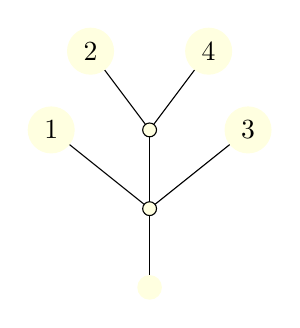
\begin{tikzpicture}
	\begin{pgfonlayer}{main}
		\node [style=inner] (3) at (0, 1) {};
		\node [style=inner] (4) at (0, 2) {};
		\node [style=leaf] (5) at (-1.25, 2) {$1$};
		\node [style=leaf] (6) at (1.25, 2) {$3$};
		\node [style=leaf] (12) at (0, 0) {};
		\node [style=leaf] (13) at (-0.75, 3) {$2$};
		\node [style=leaf] (14) at (0.75, 3) {$4$};
	\end{pgfonlayer}
	\begin{pgfonlayer}{bg}
		\draw (3.center) to (5.center);
		\draw (4.center) to (3.center);
		\draw (3.center) to (6.center);
		\draw (3.center) to (12.center);
		\draw (13.center) to (4.center);
		\draw (14.center) to (4.center);
	\end{pgfonlayer}
\end{tikzpicture}
\hspace{0.5 em}
\mathsymbol{1.5}{-}
\hspace{-1 em}
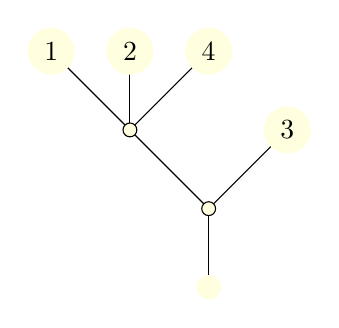
\begin{tikzpicture}
	\begin{pgfonlayer}{main}
		\node [style=inner] (0) at (0, 1) {};
		\node [style=inner] (1) at (-1, 2) {};
		\node [style=leaf] (2) at (1, 2) {$3$};
		\node [style=leaf] (3) at (-2, 3) {$1$};
		\node [style=leaf] (4) at (-1, 3) {$2$};
		\node [style=leaf] (5) at (0, 3) {$4$};
		\node [style=leaf] (6) at (0, 0) {};
	\end{pgfonlayer}
	\begin{pgfonlayer}{bg}
		\draw (3.center) to (1.center);
		\draw (4.center) to (1.center);
		\draw (5.center) to (1.center);
		\draw (1.center) to (0.center);
		\draw (0.center) to (2.center);
		\draw (0.center) to (6.center);
	\end{pgfonlayer}
\end{tikzpicture}
\]
\caption{A boundary map in $\B{\Com}$, vertices are not decorated
as there is a unique $k$-ary variable in $\Com$ for each $k\in\NN$.}
\end{figure}
At the same time, we will usually take $\PP$ to be \emph{itself}
weight graded, so that bar tree monomials have a homological
degree, which keeps track of how many elements of $\PP$ appear
in a tree monomial, and a total weight, which simply is obtained
by adding up the weights of the elements of $\PP$ in them.
We will write $\lVert T\rVert$ for the weight of a tree monomial
and use the notation $\B{\PP}_{(*)}$ when referring to this
weight grading. Thus, for example, $\B{\PP}_{(2)}$ consists of
those bar tree monomials of total weight degree two, which
can then either have homological degree one and be decorated by
one weight two element of $\PP$, or have homological degree two
and be decorated by two weight one elements of $\PP$. Note
that in general $|T|\leqslant \lVert T\rVert$.

\begin{definition}
The syzygy degree of a bar tree monomial $T$ is the difference
$\lVert T\rVert - |T|$, and we write it $\syz{T}$. We call this
the syzygy grading of $\B{\PP}$, and we use the superscript
notation $\B{\PP}^*$ when referring this this cohomological
grading: the differential $d$ has degree $+1$ in the syzygy
grading.
\end{definition}

\begin{figure}
\[
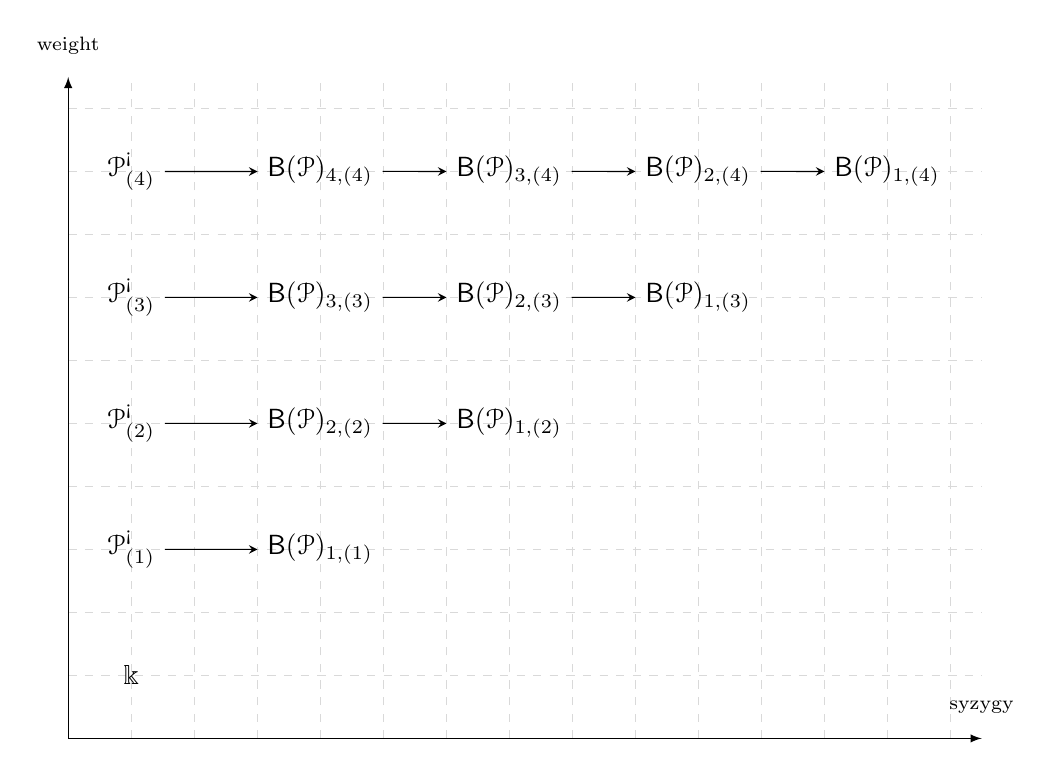
\begin{tikzpicture}[scale = 0.8]
\tikzset{>=latex}

%Draw a nice grid
\draw[help lines, color=gray!30, dashed] 
	(-4,-1) grid (10.5,9.5);

%Draw bar components 
\foreach \x in {1,2,3,4}
	{     
	\pgfmathsetmacro\result{\x} 
	\foreach \y in {1,...,\result}
	  {
	  \node (\y\x) at (3*\x - 3*\y,2*\x) {$\B{\PP}_{\y,(\x)}$};
	  	  }
	}
    {
    \draw[->,>=stealth] (22) edge (12);
    \draw[->,>=stealth] (33) edge (23);
     \draw[->,>=stealth] (23) edge (13);
    \draw[->,>=stealth] (44) edge (34);
    \draw[->,>=stealth] (34) edge (24) ;
    \draw[->,>=stealth] (24)  edge (14);

    }
   
%Draw P antishriek

\foreach \x in {1,2,3,4}
	 {
	 \node (P\x) at (-3,2*\x) {$\PP^\antishriek_{(\x)}$} ;
	 \draw[->,>=stealth] (P\x) edge (\x\x);
 }
 
 %draw lonely unit
 
 \node at (-3,0) {$\kk$};
 
 %draw some "axes"
 
 \draw[->] (-4,-1) -- (10.5,-1) ;
  \draw[->] (-4,-1) -- (-4,9.5) ;
 \node (S) at (10.5,-0.5) {\scriptsize{syzygy}};
  \node (W) at (-4,10) {\scriptsize{weight}};
 \end{tikzpicture}	
\]
\caption{The bar construction of an augmented weight graded operad $\PP$. Horizontal arrows
are differentials, leftmost arrows are inclusions. Note
that the diagonals where $s+w$ is constant return the
usual homological degree $d$. }
\end{figure}

\begin{example} Let us consider the case where $\PP = \Com$ is the
commutative operad, in which case $\XX = s\overline{\PP}$ is a symmetric
sequence such that $\XX(0) = \XX(1) = 0$ and for which $\XX(n)$ is
one dimensional for each $n\geqslant 1$ and concentrated in
degree one and weight $n-1$. It follows that $\B{\Com}$ has basis consisting
of shuffle trees where the internal vertices have
all possible arities greater or equal to $2$, and in this case the
degree of a bar tree monomial is equal to the number of 
its internal vertices. Let us write $\Gamma_m$ for the element in
$\B{\Com}$ of degree $1$ and weight $m-1$ corresponding to the 
$m$-fold product in $\Com$.

If we write $T_i(A,B)$ for the shuffle tree in
Figure~\ref{fig:twolevel}, where $A = \{ i,j_1,\ldots,j_m\}$
and $B = \{1,\ldots,i-1,k_1,\ldots,k_n\}$, we see that
$\partial T_i(A,B) = (-1)^{i-1} \Gamma_m$ where $m\geqslant 3$,
so all of these elements are zero in homology. For example, if
we look at $\B{\Com}(3)$, we notice this complex has total 
dimension four, with the usual three shuffle tree monomials
\[ T_1(12,3), 
	\quad
		T_1(13,2),
			\quad
			\text{ and  }
		 	\quad T_2(1,23)
			\]
with three leaves in degree two (and weight two) and
one single tree monomial (the corolla $\Gamma_3$) in degree one.
Moreover, the computation above shows that generators for
the homology are
\[ 
T_1(12,3) + T_2(1,23),\qquad 
T_1(13,2) + T_2(1,23)
\]
Similarly, one can compute as in Exercise~\ref{ex:barcom} that
$\B{\Com}$ is of dimension $26$, and that the degree two cycles
are of dimension $9$ (all $10$ basis shuffle trees map to the only basis
elements of degree $1$). Moreover, one can check that all of these
cycles in degree two are boundaries. Since this complex has
$\chi = 6$ and we have just noted it has homology only in
degree three, we see this homology group is of this 
dimension. We will
see very soon that in
syzygy degree zero, the homology of $\B{\Com}(n)$ 
is of dimension $(n-1)!$.
\end{example}

\subsection{Koszul dual cooperad}

Let us begin by observing that, in the syzygy grading,
$H^0(\B{\PP})$ is computed as the kernel of a linear operator,
as all syzygy degrees are non-negative (so there are no boundaries
in degree zero). We can in fact try to study the shape of the bar
construction with a little more care, and determine precisely
what this homology group is as a \emph{cooperad} in case
$\PP$ is quadratic.

To do this, let us assume that $\PP$ is generated by 
$\XX$ (in weight one) subject to some quadratic relations $\RR$ in 
$\FF_\XX^{(2)}$. Then, we see that elements of $\B{\PP}^0$ 
(that is, those that have degree equal to weight) must
be precisely those of in $\FF^c_{s\XX}$. Note the difference!
While all of $\B{\PP}$ is given by a cofree cooperad on $\PP$,
the syzygy degree zero part only retains the elements 
that generate $\PP$. 

Having said this, if we decompose 
$\FF_{s\XX}^c$ into its tree monomial components, and
if we write $\mathcal V = \FF_\XX^{(2)} / \RR$,
we see
that the differential $\partial$ maps $\FF_{s\XX}^c$ to
$\FF_{s\XX\oplus s\mathcal V}^c$, since it at
most can introduce an element of $\PP$ of weight two,
and it maps to the symmetric subsequence
$\FF_{s\XX,s\mathcal V}^c$ where
\emph{exactly one} internal vertex is decorated by an 
element of $s\mathcal V$. 

\begin{definition}
Let $\XX$ be a symmetric sequence and let $\RR\subseteq \FF_\XX^{c,(2)}$.
The cofree conilpotent cooperad cogenerated by $\XX$ subject
to the correlations $\RR$ is the unique conilpotent cooperad $\FF^c(\XX,\RR)$
that is universal among those conilpotent cooperads
$\CC$ along with a map $\CC\longrightarrow \XX$ such
that the projection of the unique map $\CC \longrightarrow \FF_\XX^c$
to $\CC \longrightarrow \FF_\XX^{c,(2)}$ has image in
$\RR\subseteq \FF_\XX^{c,(2)}$. 
\end{definition}

If the reader finds the definition slightly confusing, let us remark
that the quotient operad $\FF(\XX,\RR) = \FF_\XX/ (\RR)$ is universal
among those operads $\PP$ along with a map $\XX\longrightarrow \PP$
with the property that the restriction of the unique map 
$\FF_\XX\longrightarrow \PP$ to $\FF_\XX^{(2)}$ \emph{factors}
through $\FF_\XX^{(2)}/\RR$: whereas the condition on the operad is
that $\RR$ is contained in the kernel of this map, the condition
on conilpotent operads is that $\RR$ is contained in the image. 

\begin{proposition}
If $\PP  = \FF(\XX,\RR)$ then the zeroth
syzygy homology groups $H^0(\B{\PP})$ are equal to $\FF^c(s\XX,s^2\RR)$.
More precisely, $\CC = H^0(\B{\PP})$ is a weight graded subcooperad,
with $\CC_{(1)} = s\XX$ and the projection $\CC \longrightarrow s\XX$
satisfies the universal property of the definition above for $s^2\RR$.
\end{proposition}

\begin{proof}
First, let us note that not only is $H^0(\B{\PP})$ equal to $s\XX$ in
weight $1$, but it is also equal to $s^2\RR$ in weight $2$, as this is
by definition the kernel of the composition
\[
 \B{\PP}_{2,(2)} = \FF^{(2)}_{s\XX} \subseteq \B{\PP}^0
 	\longrightarrow 
 	s\overline{\PP}_{(2)}  \subseteq   \B{\PP}^1 
\]
so that the projection $H^0(\B{\PP})\longrightarrow s\XX$ does induce a map
$H^0(\B{\PP}) \longrightarrow \FF^c_\XX$ with the desired properties. 
Suppose that $\CC$ is a cooperad with a map $f$ to $\XX$ for which
the projection $\pi\circ F: \CC \longrightarrow \FF_\XX^{c,(2)}$ lands
in $s^2\RR$. Since $H^0(\B{\PP})$ is a subcooperad of $\FF^c_{s\XX}$,
it suffices to show that the map $F: \CC\longrightarrow \FF^c_{s\XX}$
has image in $H^0(\B{\PP}) = \ker \partial^0$.

By definition, $F$ is obtained through $f$ by iteration of the decomposition
map of $\CC$: for each $n\geqslant 1$ the component $F: \CC\longrightarrow 
\FF^{c,(n)}_{s\XX}$ in weight $n$ is obtained using $n-1$ instances of the
decomposition map of $\CC$. By hypothesis, every use of the decomposition
map of $\CC$ always creates quadratic summands that are in $\RR$, so by
coassociativity, iteration of $\Delta$ will produce terms that can be written
to contain relations in any ``big vertex'' of $\FF_{s\XX}^c$ we prefer.
This guarantees that when we apply $\partial^0$ the result will be
zero (as this is an alternating sum of terms, each which annihilates 
an appropriate way of writing down the result of iterating $\Delta$)
so that $F$ indeed lands in $H^0(\B{\PP})$, like we wanted.
\end{proof}

The reader may compare to the case of associative algebras (that is,
when $\XX$ consists exclusively of arity one operations) in which case
the cofree conilpotent coalgebra $C$ with cogenerators $V$ and relations
$R\subseteq V^{\otimes 2}$ is such that for each $n\geqslant 2$,
\[
C_{(n)} = \bigcap_{i=1}^{n-1} V^{\otimes (i-1)}\otimes R\otimes 
					V^{\otimes(n-i-1)}.
\]

\begin{definition}
Let $\PP$ be the quadratic operad associated to the quadratic datum 
$(\XX,\RR)$. We call $H^0(\B{\PP})= \FF^c(s\XX,s^2\RR)$ the Koszul dual cooperad
to $\PP$, and write it $\PP^\antishriek$.
\end{definition}

Recall that we defined $\sus = \End_{s\kk}$, the suspension operad.
We will use $\sus^c$ to denote the endomorphism cooperad $\End_{s\kk}^c$,
which we can think simply as the arity-wise dual of $\sus^{-1}$.
The ``Koszul pairing'' we used when we defined the operad $\PP^!$
gives a hint to the following result.

\begin{lemma}\label{lemma:dualcooperad}
The dual of the cooperad  $\sus^c\otimes \PP^\emph{\antishriek}$
is isomorphic to $\PP^!$.
\end{lemma}

\begin{proof}
This is Exercise~\ref{ex:dualcooperad}. 
\end{proof}

In particular, this proves that the dual operad to $H^0(\B{\Com})$ is
equal to the Lie operad, which explains the computations done and suggested
above. We can now conclude this lecture by introducing one of the
central definitions in these notes.

\begin{definition}[First definition]
A weight graded (quadratic) operad $\PP$ is Koszul if
the inclusion of cooperads $\PP^\antishriek \longrightarrow \B{\PP}$
is a quasi-isomorphism. In other words, we say that $\PP$
is Koszul if the homology of its bar construction is
concentrated in syzygy degree zero.
\end{definition}

\subsection{Exercises}	

\begin{question}
All the results in this section have a corresponding
dual statement for conilpotent cooperads. State and
prove them. In particular, define for each weight graded
cooperad $\CC$ its cobar construction $\Omega(\CC)$,
and describe the syzygy grading and the differential.
\end{question}

\begin{question}\label{ex:cofree}
Consider a binary alphabet $\XX$ with a single operation,
and compute the decomposition map of $\FF^c_\XX$ in case
this operation is symmetric, antisymmetric or regular 
for tree monomials with four leaves.
\end{question}


\begin{question}\label{ex:conilpotent}
Show that a cooperad $\CC$ is conilpotent if and only if
there exists a symmetric sequence $\XX$ and an injective
map of cooperads $\CC \longrightarrow \FF_\XX^c$. 
\end{question}

\begin{question}\label{ex:takeduals}
Show that if $\CC$ is a cooperad then its arity-wise dual $\CC^*$ 
is an operad, and that if $\PP$ is an arity-wise finite dimensional
reduced operad then its arity-wise dual $\PP^*$ is a cooperad. 
Make sure to explain why the second set of hypotheses are needed.
\end{question}

\begin{question}\label{ex:dualcooperad}
Prove Lemma~\ref{lemma:dualcooperad}, which states
that the dual of the cooperad  $\sus^c\otimes \PP^{\antishriek}$
is isomorphic to $\PP^!$.
\end{question} 

\begin{question}\label{ex:barcom}
Compute the homology of the complex $\B{\Com}(4)$ explicitly.
Show it is concentrated in syzygy degree $0$, where it is
six dimensional, and give representatives for the 
cocycles giving a basis of it.
\end{question}

\begin{question}\label{ex:zerosquare}
Show that the differential $\partial$ of the bar construction of
an augmented operad $\PP$ squares to zero if and only if the composition
map of $\PP$ is associative. 
\end{question}

\begin{question}\label{ex:dgbar} Suppose that $\PP$ is an augmented dg
operad, and let us write $\partial_1$ for the differential of its
bar construction (considered as a non-dg operad). Recall
that $s\overline{\PP}$ gets the differential $-s d_\PP s^{-1}: 
s\overline{\PP}\longrightarrow s\overline{\PP}$.

\begin{tenumerate}
\item Show that in this case the differential
of $s\overline{\PP}$ induces a differential $\partial_2$ on $\FF_{s\PP}$. 
\item Show that $\partial_1\partial_2 + \partial_2\partial_1=0$
is equivalent to $d_\PP$ being a derivation for $\gamma_\PP$.
\item
Conclude that $\partial = \partial_1 + \partial_2$ is a differential
on $\FF_{s\overline{\PP}}$. 
\end{tenumerate}
We call the resulting cooperad the bar construction of
$\PP$ and write it $\B{\PP}$.
\end{question}


 
\afterpage{\blankpage}
\newpage

\section{Koszul complexes}\label{lecture:KD2}

\textbf{Goals.} Define twisting morphisms, unravel the
bar-cobar adjunction. Give the definition of the
Koszul complexes associated to a quadratic operad,
and give a second definition of Koszulness.

\subsection{Twisting morphisms}

We begin with some more operadic algebra, this time focusing
on certain variants of the circle product that will help us
state and prove some (perhaps technical) results about
operads, conilpotent cooperads, and their (co)bar
constructions. 

\medskip

\textbf{Infinitesimal composites.}
Since we will use them often, let us define two flavours of
``infinitesimal composites''  between two symmetric sequences $\XX$ and $\YY$.
First, for a third sequence $\YY'$, let us write $\XX\circ (\YY;\YY')$
for the subfunctor of $\XX\circ (\YY\oplus \YY')$ which is linear
in $\YY'$. In other words,  we consider corollas whose root 
vertex is decorated by
$\XX$, and all whose leaves are  decorated by an element 
of $\YY$ except for one
which is decorated by an element of~$\YY'$. This construction
enjoys some sort of ``mixed functoriality'' with the usual
composition product:

\begin{definition}
Let $f:\XX \longrightarrow \XX'$ and $g: \YY\longrightarrow \YY'$
be maps of symmetric sequences. We define the infinitesimal
composite $f\circ' g$ to be the map
\[ f\circ' g: \XX\circ \YY \longrightarrow \XX'\circ (\YY;\YY') \]
such that
$(f\circ' g)(x;y_1,\ldots,y_k) = 
\sum_{i=1}^k (f(x);y_1,\ldots,g(y_i),\ldots,y_k)$.
\end{definition}

As usual, Koszul signs will appear if our sequences are dg.
We write $\XX\circ_{(1)} \YY$ for $\XX\circ (\kk,\YY)$. In other
words, we consider corollas whose root vertex is decorated by
$\XX$, and all whose leaves are ``empty'', except for one
which is decorated by an element of $\YY$. If $f$ and $g$
are as above, there is a map
\[
f\circ_{(1)} g : \XX\circ_{(1)} \YY \longrightarrow \XX'\circ_{(1)} \YY'
\]
such that $(f\circ_{(1)} g )(x;1,\ldots,1,y,1,\ldots,1) = 
 (f(x);1,\ldots,1,g(y),1,\ldots,1)$.
As we suggest,
these two constructions are better behaved than
composite product when it comes to linearity:

\begin{lemma}
For any four symmetric sequences $\XX,\YY,\YY_1,\YY_2$,
we have a natural isomorphism
\[ \XX\circ (\YY;\YY_1\oplus \YY_2) \longrightarrow 
				\XX\circ (\YY;\YY_1) \oplus \XX\circ (\YY;\YY_2).\]
In particular, if $\YY=\kk$, we have a natural isomorphism				
\[ \XX\circ_{(1)} (\YY_1\oplus \YY_2) \longrightarrow 
				(\XX\circ_{(1)} \YY_1) \oplus (\XX\circ_{(1)} \YY_2),\]
so that the functor $-\circ_{(1)}-$ is bilinear.
\end{lemma}

It is useful to remark that although $f\circ' g$ and $f\circ_{(1)} g$
look similar, they have different (co)domains and they act in different
ways on summands: while the former outputs a sum of terms, the latter
outputs one term only.

\medskip

\textbf{Infinitesimal (de)compositions.}
Let $\PP$ be a dg operad and let $\CC$ be a conilpotent
dg cooperad, and let us assume (once and for all, throughout
this section) that they are both (co)augmented. In this
situation, we can consider morphisms of dg cooperads
$\CC \longrightarrow \B{\PP}$, and we claim these
can be described purely in terms of linear maps
$\tau :\CC \longrightarrow \PP$ satisfying some conditions.

Since $\PP$ is an operad, we can then consider its 
\emph{infinitesimal composition map} $\gamma_{(1)} :\PP \circ_{(1)} 
	\PP\longrightarrow \PP$ which encodes its partial
	compositions. Similarly, we can consider the 
	infinitesimal decomposition map $\Delta_{(1)}:
\CC\longrightarrow  \CC\circ_{(1)} \CC$ obtained
by projecting the decomposition map of $\CC$ onto 
$\CC\circ_{(1)} \CC$.
\begin{figure}[h]
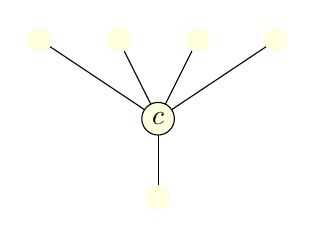
\begin{tikzpicture}
	\begin{pgfonlayer}{main}
		\node [style=leaf] (0) at (-0.5, 1) {};
		\node [circle,draw=black, fill=pagecolor, inner sep=2 pt,minimum size=6 pt] (1) at (0, 0) { $c$};
		\node [style=leaf] (2) at (-1.5, 1) {};
		\node [style=leaf] (3) at (0.5, 1) {};
		\node [style=leaf] (4) at (1.5, 1) {};
		\node [style=leaf] (12) at (0, -1) {};
	\end{pgfonlayer}
	\begin{pgfonlayer}{bg}
		\draw (2.center) to (1.center);
		\draw (1.center) to (0.center);
		\draw (3.center) to (1.center);
		\draw (1.center) to (4.center);
		\draw (1.center) to (12.center);
	\end{pgfonlayer}
\end{tikzpicture}
\mathsymbol{1.5}{\leadsto}
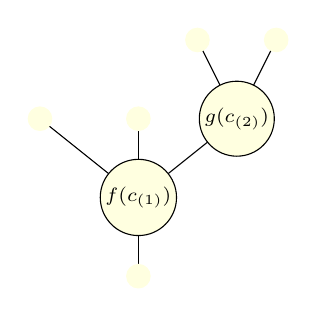
\begin{tikzpicture}
	\begin{pgfonlayer}{main}
		\node [style=leaf] (0) at (0, -1) {};
		\node [style=inner] (1) at (0, 0) {\scriptsize $ f(c_{(1)})$};
		\node [style=leaf] (2) at (-1.25, 1) {};
		\node [style=leaf] (3) at (0, 1) {};
		\node [style=inner] (4) at (1.25, 1) {\scriptsize $ g(c_{(2)})$};
		\node [style=leaf] (5) at (0.75, 2) {};
		\node [style=leaf] (6) at (1.75, 2) {};
	\end{pgfonlayer}
	\begin{pgfonlayer}{bg}
		\draw (2.center) to (1.center);
		\draw (1.center) to (3.center);
		\draw (5.center) to (4.center);
		\draw (4.center) to (6.center);
		\draw (4.center) to (1.center);
		\draw (1.center) to (0.center);
	\end{pgfonlayer}
\end{tikzpicture}
	\mathsymbol{1.5}{\leadsto}
	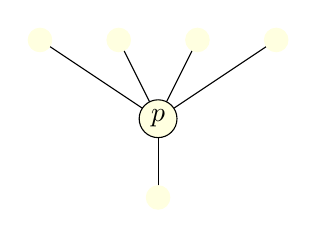
\begin{tikzpicture}
\begin{pgfonlayer}{main}
		\node [style=leaf] (0) at (-0.5, 1) {};
		\node [circle,draw=black, fill=pagecolor, inner sep=2 pt,minimum size=6 pt] (1) at (0, 0) {$p$};
		\node [style=leaf] (2) at (-1.5, 1) {};
		\node [style=leaf] (3) at (0.5, 1) {};
		\node [style=leaf] (4) at (1.5, 1) {};
		\node [style=leaf] (12) at (0, -1) {};
	\end{pgfonlayer}
	\begin{pgfonlayer}{bg}
		\draw (2.center) to (1.center);
		\draw (1.center) to (0.center);
		\draw (3.center) to (1.center);
		\draw (1.center) to (4.center);
		\draw (1.center) to (12.center);
	\end{pgfonlayer}
	\end{tikzpicture}
\caption{A schematic version of the star product: we use ``Sweedler notation'' for
the infinitesimal decomposition of $\CC$ and write $p$ a generic
summand $f(c_{(1)})\circ_i g(c_{(2)})$ appearing in the final result.}
\label{fig:starprod}
\end{figure}
\begin{definition}
Let $f,g\in \hom_\Sigma(\CC,\PP)$ be maps of symmetric
sequences. We define their star product $f\star g$ 
as the composition
$\gamma_{(1)} \circ (f\circ_{(1)} g)\circ \Delta_{(1)}$,
as depicted in Figure~\ref{fig:starprod}. We give 
$\hom_\Sigma(\CC,\PP)$ the usual differential
\[
\partial(f) = d_\PP \circ f  - (-1)^{|f|} f\circ d_\CC.
\]
\end{definition}

One can show that $\hom_\Sigma(\CC,\PP)$ along with
the star product $-\star -$ becomes a pre-Lie algebra,
 which is dg if $\CC$ or $\PP$ are. By anti-symmetrizing
 $-\star -$, we thus obtain a dg Lie algebra structure
 on $\hom_\Sigma(\CC,\PP)$. As in any dg Lie algebra,
 the degree $-1$ elements satisfying a particular equation
 play an important role and, for historical reasons,
  we give them a name here 
 different from the usual ``Maurer--Cartan element'':
 
\begin{definition}
We write $\Tw(\CC,\PP)$ for the set of degree $-1$ maps
$\tau : \CC\longrightarrow \PP$
such that $\tau\eta =0$, $\varepsilon\tau = 0$
and 
\[
\partial(\tau) + \tau\star \tau = 0,
\]
and call it the set of \emph{twisting morphisms} from
$\CC$ to $\PP$. We call the equation in the display the
\emph{Maurer--Cartan equation} for $\tau$.
\end{definition}


\subsection{Adjunction}
The bar construction admits a dual construction for
coaugmented conilpotent cooperads $\CC$, which we call
the cobar construction and write $\Omega(\CC)$. These
two functors fit into a diagram
\[
 \Omega(-)  : \mathsf{Coop}^c   \adjoint
  \mathsf{Op} :\B{-}
\]
from the category of augmented operads (which we may allow to be
dg, see Exercise~\ref{ex:dgbar}) to the category of
\emph{conilpotent} augmented dg cooperads. The following
theorem can be considered as one of the incarnations of Koszul
duality between operads and conilpotent cooperads.

\begin{theorem}\label{thm:adjunction}
The bar and cobar functors form an adjoint pair
$ \Omega(-)  : \mathsf{Coop}^c   \adjoint
  \mathsf{Op} :\B{-}$.
More precisely, 
for every operad $\PP$ and every conilpotent cooperad
$\CC$, the following are in natural bijection:
\begin{tenumerate}
\item Maps of conilpotent dg cooperads $\CC \longrightarrow \B{\PP}$.
\item Maps of dg operads $\Omega(\CC) \longrightarrow\PP$.
\item Twisting morphisms $\CC \longrightarrow \PP$.
\end{tenumerate}
\end{theorem}

\begin{proof}
Let us consider a map $f : \CC \longrightarrow \B{\PP}$ of cooperads
with $\CC$ conilpotent. Forgetting for the moment that the codomain
has a differential, we notice that there exists a unique map of
symmetric collections $\CC \longrightarrow s\overline{\PP}$
that induces it. Equivalently, there is a degree $-1$ map
$\tau : \CC \longrightarrow \PP$ such that $\varepsilon\tau = 0$
and $\tau\eta = 0$ (this second equality follows since $\B{\PP}$ is
augmented and connected)
which induces $f$. The fact that $f$ commutes with the differential of
$\B{\PP}$ is equivalent to the Maurer--Cartan equation
\[
\partial \tau + \tau\star\tau = 0.
\]
The degree $-1$ map $\tau : \CC\longrightarrow \PP$ in turn can
be turned into a degree zero map $s^{-1}\overline{\CC}\longrightarrow
\PP$ which, by the universal property of the free operad construction
induces a map $\Omega(\CC) \longrightarrow \PP$, which in fact commutes with
the differential, as one can check this is also equivalent
to the equation above. We conclude that the two hom-sets in
the statement of this theorem are in bijection with the set
of symmetric sequence morphisms $\tau : \CC\longrightarrow \PP$
that satisfy the above Maurer--Cartan equation and
such that both $\tau\eta$ and $\varepsilon\tau$ vanish,
which are precisely the twisting morphisms we have defined.
\end{proof}

Since it will be useful for us, let us make the bijection
in the theorem above more explicit. To do this, let us consider
the map $\pi : \B{\PP} \longrightarrow \PP$ obtained
as the projection onto $s\overline{\PP}$ and the degree
$-1$ inclusion into $\PP$. Then the bijection
\[
\hom_{\mathsf{Coop}^c}(\CC,\B{\PP})
 	\longrightarrow
 	 \mathsf{Tw}(\CC,\PP)
\]
is given by post-composition with $\pi$, while the
inverse is given by extending the
resulting degree zero map 
$\CC\longrightarrow \PP$ to a unique coderivation
$\CC\longrightarrow \B{\PP}$. We call $\pi$
the universal twisting cochain (it is one, as per
Exercise~\ref{ex:universaltw}), and observe that it
corresponds to the identity map of $\B{\PP}$ under
the bijection above. 

Dually, there is a degree $-1$ inclusion $\iota:
\CC\longrightarrow \Omega(\CC)$ which is also a 
twisting cochain ---the universal twisting cochain
for the conilpotent cooperad $\CC$--- and the bijection
\[
\hom_{\mathsf{Op}}(\Omega(\CC),\PP)
 	\longrightarrow
 	 \mathsf{Tw}(\CC,\PP)
\]
is given by pre-composition with $\iota$. To summarize,
for any map $\CC\longrightarrow \PP$ we have a commutative
diagram
\[
\begin{tikzcd}
{} & \Omega(\CC) \arrow[dr] & {} \\
\CC \arrow[ur,"\iota"]
	\arrow[dr]
	\arrow[rr,"\tau"] & {} & \PP \\
{} & \B{\PP} \arrow[ur,"\pi",swap] & {} 
\end{tikzcd}
\]
where the diagonal maps are the universal twisting cochains, 
the anti-diagonal maps are maps of dg (co)operads and
the only horizontal arrow is the corresponding twisting cochain.
In other words, every twisting cochain $\CC\longrightarrow \PP$
factors uniquely as the composition of the universal twisting
cochain $\iota$ followed by a morphism of dg operads, and
as the composition of a morphism of dg conilpotent cooperads
followed by the universal twisting cochain $\pi$.

\subsection{Koszul complexes}

\textbf{Left and right modules over operads.} Since it will be useful
later, let us begin by noticing that operads admit representations other
than their algebras (which we introduce in the Appendix). We will
use this to define certain objects that are central to our lectures:
the Koszul complexes of twisting cochains.

\begin{definition}
Let $\PP$ be an operad. A right $\PP$-module is a symmetric
sequence $\MM$ along with a map $\rho :\MM\circ\PP\longrightarrow \MM$
that is unital and associative for the unit and the composition
map of $\PP$, that is, the following diagrams commute:
\[
\begin{tikzcd}
(\MM\circ \PP)\circ \PP 
	\arrow[r,"\rho\circ 1"]
	\arrow[dd,"\alpha",swap] 				& \MM\circ \PP \arrow[dr,"\rho"] \\
	{} 						& {} 			& \MM\\
\MM\circ (\PP \circ \PP) \arrow[r,"1\circ\gamma"] & 
	\MM \circ \PP \arrow[ur,"\rho",swap]
\end{tikzcd}
\qquad
\begin{tikzcd}
\MM\circ \kk \arrow[dd,"1\circ\eta",swap] \arrow[dr,"\cong"] & {} \\
 {}                               &  \MM \\
\MM\circ \PP \arrow[ur,"\rho",swap]
\end{tikzcd}
\]
A map of right $\PP$-modules is a morphism
of symmetric sequences $f:\MM\longrightarrow \MM'$ 
such that the following diagram commutes:
\[
\begin{tikzcd}[row sep = large, column sep = large]
\MM\circ \PP \arrow[r,"\rho"]
	\arrow[d,"f\circ 1",swap] & \MM \arrow[d,"f"]\\
\MM'\circ \PP \arrow[r,"\rho'",swap] & \MM'
\end{tikzcd}
\]
Finally, a free right $\PP$-module is any module that is isomorphic
to one of the form $\MM = \XX\circ\PP$ where the map $\rho : \MM\circ\PP
\longrightarrow \MM$ is given by the composition
\[
(\XX\circ \PP)\circ\PP 
\stackrel{\alpha}{\longrightarrow}
\XX \circ (\PP \circ \PP) 
	\stackrel{1\circ\gamma}{\longrightarrow} 
		\XX\circ \PP.
\]
\end{definition}

\emph{Note.} If we replace the word ``right'' above by ``left'' we obtain
the corresponding definitions for \emph{left $\PP$-modules}. A word of
caution is in order, however, as right modules and left modules in
case of operads behave completely differently. For example, right
actions are linear, in the sense that their signature is of the
form
\[
(m;p_1,\ldots,p_k) \longrightarrow \rho(m;p_1,\ldots,p_k)
\] 
and in particular there is only one argument in $\MM$. On the
other hand, left actions are not linear, in the sense that their
signature is of the form
\[
(p;m_1,\ldots,m_k) \longrightarrow \lambda(p;m_1,\ldots,m_k)
\] 
for multiple $m_1,\ldots,m_k\in \MM$: an element in $\PP$
of arity $k$ must act simultaneously on $k$ elements of $\MM$
at once and, since modules have no units, there is no way
to linearize this. We will have the opportunity to see
how this distinction will affect our development of the
theory in some cases.

\begin{definition}
Let $\MM$ be a left $\PP$-module. An endomorphism
$f: \MM \longrightarrow \MM$ of symmetric sequences is
called a derivation if for all $m_1,\ldots,m_k\in\MM$
and $p\in\PP(k)$ we have that $f \lambda = \lambda(1\circ' f)$
\end{definition}
 
In the case of right $\PP$-modules, there is no difference
between a derivation and a right linear map ---in both cases
the relevant requirement is that $f\rho = \rho(f\circ 1)$---, but we will use
both names for consistency. Note that the condition above of
being a derivation is linear, as $f$ appears only once in each
use of $\lambda$, so left linear maps and left derivations
are slightly different. However, they are in natural bijection
when we restrict ourselves to the class of free modules:

\begin{lemma}\label{lemma:derivations}
Let $\PP$ be an operad and let $\MM$ be a free
left (resp. right) $\PP$-module with basis $\XX$.
There is a natural bijection between maps of 
symmetric sequences $\XX\longrightarrow \MM$
and left (resp. right) derivations $\MM\longrightarrow \MM$.
More precisely:
\begin{tenumerate}
\item If $\MM$ is left free, then the unique derivation $f:\MM\longrightarrow\MM$
which extends $\varphi: \XX\longrightarrow \MM$ is given by
\[
f = d_\PP \circ 1 + (\gamma_{(1)}\circ 1)(1\circ'\varphi).
\]
\item  If $\MM$ is right free, then the unique derivation $f:\MM\longrightarrow\MM$ 
which extends $\varphi: \XX\longrightarrow \MM$ is given by
\[
f = 1\circ' d_\PP  + (1\circ\gamma)(\varphi\circ 1).
\]
\end{tenumerate}
\end{lemma}

\textbf{Koszul complexes.}
Let $\tau : \CC\longrightarrow \PP$ be a twisting cochain,
and let us explain how to produce a map that assigns $\tau$
two complexes $\CC\circ_\tau \PP$ and $\PP\circ_\tau\CC$, 
the \emph{right (resp. left) Koszul complex} associated to $\tau$.
In the first case, let us consider the free right $\PP$-module
$\CC\circ \PP$, and let us consider the map
$\CC \longrightarrow \CC\circ \PP$
obtained as the composition $(1\circ_{(1)} \tau)\Delta_{(1)}$.
By Lemma~\ref{lemma:derivations}, there is a unique derivation
of right $\PP$-modules
$d_\tau^r : \CC\circ \PP \longrightarrow \CC\circ \PP$
extending the map above. It is given by the following composition:
\[
\begin{tikzcd}[column sep = large]
{} & (	\CC\circ_{(1)} \CC )\circ\PP \arrow[r,"(1\circ_{(1)}\tau)\circ 1"] 
	& (	\CC\circ_{(1)} \PP )\circ
	\PP  \arrow[dr,"\cong"]\\ 
\CC\circ \PP \arrow[ur,"\Delta_{(1)}\circ 1"]\arrow[dr,"d_\tau^r",swap] & {} & {} & \CC\circ (\PP;\PP\circ\PP)\arrow[dl,"1\circ(1;\gamma)"]\\ 
{} &  \CC\circ \PP &  \CC\circ (\PP;\PP)\arrow[l,"\cong"] &{}
\end{tikzcd}
 \]
Dually, we write $d_\tau^l$ for the unique derivation of the free left 
$\PP$-module $\PP\circ\CC$ extending the map $\CC\longrightarrow \PP\circ \CC$
given by the composition $(\tau\circ 1)\Delta$. 


\begin{proposition}
The derivation $\partial_\tau = d_\CC\circ 1  + 1\circ' d_\PP + d_\tau^r$
of $\CC\circ \PP$
is such that $\partial_\tau^2 = d_{\partial(\tau) + \tau\star\tau}^r$. In 
particular, it squares to zero if and only if $\tau$ is a twisting
morphism. Similarly, the derivation  $\partial_\tau = d_\PP\circ 1  + 1\circ' 
d_\CC + d_\tau^l$ of $\PP\circ \CC$ is such that 
$\partial_\tau^2 = d_{\partial(\tau) + \tau\star\tau}^l$,
so that it squares to zero if and only if $\tau$ is a twisting
morphism.
\end{proposition}

\begin{proof}
The proof involves a computation, though the computation may get
rather cumbersome, so we provide the requisite
details
in the Appendix. In fact, we will
prove something a bit stronger: the assignment that takes 
a morphism $\tau : \CC\longrightarrow \PP$ of symmetric
sequences to the derivation $d_\tau^r : \CC\circ\PP \longrightarrow
\CC\circ \PP$ is a morphism of dg Lie algebras, where we put
on $\hom_\Sigma(\CC,\PP)$ the dg Lie algebra structure induced by
the pre-Lie star product $-\star-$ and we give the space of
derivations $\operatorname{Der}(\CC\circ\PP)$ the usual
structure of a Lie algebra through the commutator of
derivations (recall that the composition of two derivations
need not be a derivation, but the commutator of derivations
is a derivation).

To see how this claim implies the proposition, we notice
that $\partial_\tau\circ\partial_\tau = \frac{1}{2}[\partial_\tau,\partial_\tau]$
and that if we write $\partial_\tau = d_{\CC\circ\PP} + d_\tau^r$, then
\begin{tenumerate}
\item The original differential squares to zero, so that $[d_{\CC\circ\PP},d_{\CC\circ\PP}] = 0$,
\item The fact this is a morphism of complexes shows that $[d_{\CC\circ\PP},d_\tau^r] = d_{\partial(\tau)}^r$ and,
\item The claim above proves that $[d_\tau^r,d_\tau^r] = d_{[\tau,\tau]}^r$.
\end{tenumerate}
This completes the proof of the proposition.
\end{proof}

\begin{definition}
We write $\CC\circ_\tau \PP$ for the complex in right $\PP$-modules
$(\CC\circ \PP,\partial_\tau)$, and call it the \emph{right Koszul
complex associated to $\tau$}. Analogously, we write $\PP\circ_\tau \CC$
for the complex in free left $\PP$-modules $(\PP\circ \CC,\partial_\tau)$
and call it the \emph{left Koszul complex associated to $\tau$}.
\end{definition}

We are now ready to make concrete our claim that Koszul (co)operads are
those that admit economic resolutions: we did not say of \emph{what}
object, but we can do that now. The only observation we need to make
is the following:

\begin{definition}
Let $\PP$ be a quadratic operad. The map $\kappa : \PP^\antishriek
\longrightarrow \PP$ obtained as the composition
$\PP^\antishriek \hookrightarrow \B{\PP} \longrightarrow \PP$
is a twisting cochain.
\end{definition} 

Note that $\kappa$ can be described even in simpler terms as
the degree $-1$ map obtained as the compositions of the projection
$\PP^\antishriek \twoheadrightarrow s\XX$ onto weight $1$,
the desuspension map $s\XX\stackrel{s^{-1}}\longrightarrow \XX$
and the inclusion $\XX \hookrightarrow \PP$. 

\begin{proof}
This is actually a straightforward computation,
since in our situation $\PP$ has no differential
and we only need to show that $\kappa\star \kappa = 0$. 
But $\kappa\star\kappa : \PP^\antishriek \longrightarrow \PP$
is obtained as the composition
\[
\PP^\antishriek\stackrel{\Delta_{(1)}}\longrightarrow 
 	\PP^\antishriek \circ_{(1)} 	\PP^\antishriek 
 	 \longrightarrow
 	 	\PP \circ_{(1)} 	\PP 
 	 		\stackrel{\gamma_{(1)}}\longrightarrow 
 	 		\PP
\]
where the map $\kappa\circ_{(1)} \kappa$ in the middle is only non-zero
on elements of $s\XX\circ_{(1)} s\XX \subseteq \PP^\antishriek\circ_{(1)} \PP^\antishriek$, and in this case the decomposition of $\PP^\antishriek$
lands on $s^2\mathcal R$ by construction. This means that
the image after using the composition map of $\gamma$ lands in $\RR$,
which is zero in $\PP$, as we claimed.
\end{proof}

With this at hand, here is our second definition of Koszulness.
By Theorem~\ref{thm:fundamental} in the Appendix, the following
is equivalent to our original definition of Koszulness of a quadratic
operad, stating that the inclusion $\PP^\antishriek \longrightarrow 
\B{\PP}$ is a quasi-isomorphism of cooperads. 

\begin{definition}[Second definition]
A quadratic operad $\PP$ is Koszul if and only if the
right Koszul complex $\PP^\antishriek \circ_\kappa \PP$
is a resolution of the trivial module $\kk$ in right
$\PP$-modules. Equivalently, 
a quadratic operad $\PP$ is Koszul if and only if the
left Koszul complex $\PP \circ_\kappa \PP^\antishriek$
is a resolution of the trivial module $\kk$ in left
$\PP$-modules.
\end{definition}

\subsection{Exercises}

\begin{question}
Suppose that $\PP$ is locally finite dimensional and that $\PP(1) = \kk$. 
Show that $\B{\PP}$ and $\Omega(\PP^*)$ are dual to each other.
\end{question}

\begin{question}
Prove the claim in Theorem~\ref{thm:adjunction} that the Maurer--Cartan
equation for the map $\tau : \CC\longrightarrow \PP$ corresponding
to a morphism of dg cooperads $f : \CC\longrightarrow \B{\PP}$
and to a morphism of dg operads $g  :\Omega(\CC) \longrightarrow \PP$
is equivalent to the condition that $f$ and $g$ commute with the
differentials.
\end{question}


\begin{question}\label{ex:universaltw}
Show that the universal twisting cochain
$\pi:\B{\PP}\longrightarrow \PP$ is indeed
a twisting cochain, and that the Maurer--Cartan
equation is equivalent to the condition that 
$\PP$ is a dg operad. Do the same for the 
 universal twisting cochain $\iota : \CC 
\longrightarrow \Omega(\CC)$, and 
\end{question}


\begin{question}
Show that $\PP \longmapsto \pi_\PP$ is natural, in
the sense that for a morphism of operads $\PP\longrightarrow 
\PP'$ we have a commutative square
\[
\begin{tikzcd}[ampersand replacement=\&]
\B{\PP} \arrow[r] \arrow[d] \&  \PP \arrow[d] \\
\B{\PP'} \arrow[r] \& \PP'
\end{tikzcd}
\]
Do the same for $\iota$. Show that the bijection described in Theorem~\ref{thm:adjunction} 
is natural.  
\end{question}
\afterpage{\blankpage}
\newpage


\section{Methods to prove an operad is Koszul I}\label{lecture:methods1}

 \subsection{Monomial operads}
 
Let us fix a shuffle operad $\PP$ generated by some set of
variables $\XX$ subject to some relations $\RR$ determined
by tree polynomials, and suppose that $\prec$ is an admissible
monomial order on $\FF_\XX^\Sha$. With this information, one
can consider the operad $\PP_\mathrm{mon}$, generated by
the same variables $\XX$ but by the tree monomials 
$\leadm{\RR}$, sometimes denoted $\mathrm{in}_\prec(\RR)$
in the cases of associative (or associative commutative) algebras.
We call it the monomial operad associated to  $\PP$.

If we let $\mathcal N$ denote the subsequence of $\FF_\XX$ 
generated by the normal forms for this order with respect to $\RR$,
we have an isomorphism of collections $\PP_\mathrm{mon} \cong \mathcal N$
and, at the same time, a map of sequences
\[
\eta : \PP_\mathrm{mon} \longrightarrow \PP 
\]
obtained as the composition of the inclusion $\mathcal N\subseteq
\FF_\XX$ with the projection $\FF_\XX^\Sha\longrightarrow \PP$. One observation
we can begin to make is the following.

\begin{lemma} The composition $\PP_\mathrm{mon}\xrightarrow{\cong} \mathcal N \hookrightarrow 	\FF_\XX^\Sha \twoheadrightarrow \PP$
is an isomorphism of collections if, and only if, the set of relations 
$\RR$ is a Gr\"obnber basis for $\PP$. 
\end{lemma}

\begin{proof}
The normal forms generate $\PP$ if and only if this map is surjective, which simply
amounts to the statement that every tree polynomial can be reduced
modulo $\RR$ to a normal form: this is always true, since we have
available to us the long division algorithm. At the same time,
this map is injective if and only if every tree polynomial has a unique normal form
modulo $\RR$, which is precisely the condition that our set of
relations constitutes a Gr\"obner basis.
\end{proof}

Thus, one can think of monomial operads (shuffle, symmetric, or ns) 
as certain pivotal objects that have a simpler ``multiplication table''
than generic operads, and can be used as a first approximation to studying
these latter objects. More precisely, one can in general prove that the
homotopy type of an algebraic operad with a Gr\"obner basis can be obtained
by perturbing the homotopy type of the corresponding monomial operad,
which allows to make concrete informal claims such as the previous one.
Since we are interested in studying quadratic operads, 
let us begin by studying quadratic monomial operads and to do so,
let us introduce them proper.

\begin{definition}
Let $\XX$ be a set collection, and let $\RR$ be a set of tree monomials
in $\FF_\XX$. We call $\FF(\XX,\RR)$ the monomial operad associated to the
datum $(\XX,\RR)$. 
\end{definition}

Note that, just like in the case of associative algebras, one can apply
a linear change of coordinates to a monomial operad to obtain an operad
that is not presented by relations that are tree monomials. We will only
consider monomial operads with a given presentation or, what is the same,
``monomial data'' $(\XX,\RR)$ as above.

\begin{lemma}
Let $(\XX,\RR)$ be a shuffle quadratic monomial datum, and let us write
$(\XX^\vee,\RR^\perp)$ for the Koszul dual datum. 
\begin{tenumerate}
\item The shuffle tree monomials
not divisible by any element of $\RR$ form a linear basis of
$\PP = \FF(\XX,\RR)$.
\item  The set of shuffle tree monomials for which every
quadratic divisor belongs to $\RR$ forms a basis of $\PP^!$.
\end{tenumerate} 
\end{lemma}

\begin{proof}
This is a particular case of Exercise~\ref{ex:quadratic-GB-dual}.
\end{proof}

Let us now describe the right Koszul complex of a quadratic monomial operad
and show that quadratic monomial operads are Koszul.

\begin{theorem}
Quadratic monomial operads are Koszul
\end{theorem}

\begin{proof}
Let $\PP$ be the monomial operad associated to a monomial datum $(\XX,\RR)$.
The right Koszul complex $\PP^\antishriek\circ\PP$ has a basis consisting
of all shuffle tree graftings of the form
\[ x = \gamma_{\pi}(T; T_1,\ldots,T_k) 
\]
where $T$ is a shuffle tree not divisible by any monomial in $\RR$ and
$T_1,\ldots,T_k$ are shuffle trees all whose quadratic divisors are in $\RR$.
The differential acts by first extracting a variable from $T$, that is,
applying $\Delta_{(1)}$ and then $\tau$ at the top, and then grafting this
variable with the corresponding trees at the top. If the resulting tree 
is divisible by a relation, it is zero in $\PP$, and this term vanishes,
and if not, it remains a basis element of $\PP$. Note that $dx$ will 
contain several summands. 

In parallel, let us consider the degree $+1$ map $h$ on $\PP^\antishriek\circ\PP$
that takes a grafting $x$ and, for the first $T_i$ that can be written as a
grafting $\gamma_{1,2}(v ; T',T'')$ for $v$ a variable, replaces
$T$ by the tree $\tilde{T}$ obtained by grafting $v$ on $T$, to obtain the element
\[
\gamma_{\tilde{\pi}}(\tilde{T}; T_1,\ldots,T_{i-1},T',T'',\ldots,T_k).
\]
We send this element to zero if $\tilde{T}$ is not in $\PP^\antishriek$
and to itself otherwise. One can check that $hd + dh = 1-\iota\pi$, 
where $\pi$ is the projection onto $\kk$ in arity $1$ and $\iota$ the 
corresponding inclusion, so we obtain a contracting homotopy for our complex.
\end{proof}
\subsection{The numerical criterion}

\textbf{Hilbert and Poincar\'e series.} Let us begin
by presenting a numerical criterion that can give a \emph{negative}
answer to the question ``Is this operad Koszul?''. This
depends on certain invariants associated to chain complexes
and graded modules, which we now introduce.

\begin{definition}
Let $\XX$ be a locally finite reduced symmetric sequence
Its \emph{Hilbert series} is the formal power-series
\[
h_\XX(z) = \sum_{n\geqslant 1} \dim \XX(n) \frac{z^n}{n!}.
\]
If $\XX$ is weight graded (so that we may assume that each
weight component is locally finite) we can consider the two
variable Hilbert series
 \[
h_\XX(z,u) = \sum_{w\geqslant 0} h_{\XX^{(w)}}(z) u^w.
\]
\end{definition}

We will mainly be interested in the case of a weight graded operad $\PP$.
When $\PP$ is binary quadratic, the arity $n$ and the weight $w$ are related
by $n = w+1$ and then the two variable Hilbert series carries no new information.
For example, we can compute the following Hilbert series:
\begin{align*}
h_{\As}(z) &=  z + z^2 + z^3 + \cdots = \frac{z}{1-z} \\
h_{\Lie}(z) &=  z + \frac {z^2}2 + \frac{z^3} 3 + \cdots =-\log(1-z) \\
h_{\Com}(z) &=  z + \frac {z^2}2 + \frac{z^3} 6  + \cdots = \exp z -1 \\
h_{\As^-}(z) &=  z +  {z^2} + z^3.
\end{align*}

%Let $(C,d)$ be a chain complex. Its Euler characteristic (when defined)
%is the integer $\chi(C) = \sum_{n\in \mathbb Z} (-1)^n \dim C_n$. 

There is a related invariant, which we now define:
\begin{definition} Let $\PP$ be a weight graded operad, so that
$\B{\PP}$ is a weight graded dg cooperad. The Poincar\'e series
of $\PP$ is, by definition,
\[
p_{\PP}(z,u,t) = \sum_{w,d\geqslant 0,} \dim H_d(\B{\PP}^{(w)}(n)) t^d u^w z^n/n!.
\]
\end{definition}

We can now state and prove a numerical criterion to check if an
operad is \emph{not} Koszul.

\begin{theorem}
Let $\PP$ be a weight graded (non-dg) operad. Then we have the following
functional equation between the Hilbert and the Poincar\'e series of $\PP$:
\[
h_\PP( p_\PP(z,u,-1),u) = p_\PP(h_\PP(z,u),u,-1) = z. \]
Moreover, $\PP$ is Koszul (and in particular, quadratic) if and only
if $p_\PP(z,u,t) = -h_{\PP^\eantishriek}(z,ut)$ in which case the previous
equation simplifies to
\[
h_\PP( h_{\PP^\eantishriek}(z,-u),u) = h_{\PP^\eantishriek}(h_\PP(z,u),-u) = z. 
\]
\end{theorem}

\begin{proof}
Let us begin by proving the first functional equation. In this case,
we can consider the two augmented bar complexes of Theorem~\ref{thm:augacyclic},
of the form
\[
\PP\circ\B{\PP},\qquad \B{\PP}\circ\PP. 
\]
That theorem states these two complexes are acyclic, which means their
(weight graded) Euler characteristics are equal to the Euler characteristic 
of the symmetric sequence $(0,\kk,0,\ldots)$ where $\kk$ is placed in arity one,
weight zero, and homological degree zero, so that its Euler characteristic is
$z$. On the other hand, the Euler characteristic of $\B{\PP}$ is
$p_\PP(z,u,-1)$ and that of $\PP$ is its Hilbert series (since $\PP$ carries no
homological degrees). Thus, we obtain that 
\[
z = \chi(\PP\circ\B{\PP}) = \chi(\PP)\circ \chi(\B{\PP}) = 
		h_\PP(p_\PP(z,-1)),
\]
while $z = p_\PP(h_\PP(z),-1)$ is proved in the same fashion. Suppose
now that $\PP$ is Koszul, which means that $\dim H_d(\B{\PP})_{(w)} = 0$
unless $w=d$. This is true if and only if the coefficient of $z^wu^d$ in
$p_\PP(z,u)$ is zero unless $w=d$, in which case we have that
$H_d(\B{\PP})_{(d)} \simeq  \PP^\antishriek_{(d)}$ and
\[
p_\PP(z,u,t) = \sum_{d\geqslant 0} \dim \PP^\antishriek_{(d)}(n) 
	\frac{z^n}{n!} (tu)^d = h_{\PP^\antishriek}(z,tu).
\]
Plugging this back into the equation relating the Hilbert and Poincar\'e
series for $\PP$ gives us the result.
\end{proof}

At this point it is useful to come back to the situation when $\PP$
is binary and quadratic, in which case the functional equation
simplifies even further. In this case, we notice that
$h_\PP(z,u) = u h_\PP(zu,1)$ so we obtain the equations  
\[
h_\PP(-h_{\PP^\antishriek}(-z)) = h_{\PP^\antishriek}(-h_\PP(-z)) = z. 
\]
Since $\PP^!$ and $\PP^\antishriek$ have the same Hilbert series (even
though one is homologically graded and the other is not, we are
ignoring the $t$ variable here) we will use the functional equation above
when with the operad $\PP^!$ most of the time.



\begin{example}
The quadratic operad $\As^-$ of anti-associative algebras is not Koszul.
Indeed, one can compute the first few terms of its sign-modified inverse of the 
Hilbert series to obtain
\[
z + z^2 + z^3  - 4 z^5 + \textrm{O}(z^{6}).
\]
Since the coefficient of $z^{5}$ is negative, we conclude that this operad cannot be Koszul. 
\end{example}

%
%\begin{example}
%The quadratic operad $\As^-$ of anti-associative algebras is not Koszul.
%Indeed, one can compute the first few terms of its sign-modified inverse of the 
%Hilbert series to obtain
%\[
%z + z^2 + \frac{3}{2}z^3  + \frac 52 z^4 + \frac{17}4 z^5  + 7z^6 + 
%	\frac{21}{2} z^7 + \frac{99}8 z^8
%+ \frac{55}{16} z^9 - \frac{715}{16} z^{10}  + \textrm{O}(z^{11}).
%\]
%Since the coefficient of $z^{10}$ is negative, we conclude that this operad
%cannot be Koszul. 
%\end{example}

\begin{example}
The quadratic operad $\mathsf{Nov}$ of Novikov algebras is not Koszul.
Indeed, A. Dzhumadil'daev computed that $\mathsf{Nov}$ has the same Hilbert
series $h(z)$ as its Koszul dual, and that 
 \[ h(-h(-z)) = z + \frac 16 z^5 + \mathrm{O}(z^6) \neq z.
 \] 
 Thus, the Novikov operad is not Koszul.
\end{example}


 
\subsection{Exercises}

\begin{question}
Use the Haskell Calculator to show that $\mathsf{Nov}$ has Hilbert series
\[
h_\mathsf{Nov}(z) = z +2 \frac{z^2}{2!} +6 \frac{z^3}{3!} + 20 \frac{z^4}{4!} + 70 \frac{z^5}{5!} +
\mathrm{O}(z^6).
\]
Show that $\mathsf{Nov}$ is Koszul dual to $\mathsf{Nov}^\mathrm{op}$
and conclude that $\mathsf{Nov}$ is not Koszul.
\end{question}
\begin{question}\label{ex:preLieHilbert}
Show (using Gr\"obner bases or otherwise) that the Hilbert series $h$
of the operad $\mathsf{PreLie}$ satisfies the equation
\[ h(z) = z\exp h(z) .\]
Use this to compute a few terms of the series, or directly
show that $\dim\mathsf{PreLie}(n) = n^{n-1}$. Compute
the Hilbert series of $\mathsf{Perm}$ and verify that
the numerical criterion holds.
\end{question}

\begin{figure}

\begin{verbatim}

Configuration:

actions:        normalise count 
count limit:    5
arity limit:    5
time limit:     none
output:         
field:          rationals
operad type:    unsigned shuffle operad
measure:        permutation reverse degree-lexicographic 
signature:      x(2) y(2)
theory:
  x(x(1 3) 2)  -  x(x(1 2) 3)
  y(1 x(2 3))  -  x(y(1 2) 3)
  y(1 y(2 3))  -  x(y(1 3) 2)
  x(x(1 2) 3)  -  x(1 x(2 3))  -  x(y(1 2) 3)  +  y(x(1 3) 2)
  x(x(1 3) 2)  -  x(1 y(2 3))  -  x(y(1 3) 2)  +  y(x(1 2) 3)
  y(1 x(2 3))  -  y(y(1 3) 2)  -  y(1 y(2 3))  +  y(y(1 2) 3)


Arity: 4   
Stable rewrite rules: 6   
Current critical pairs: 26   
Queued critical pairs: 0

Arity: 5   
Stable rewrite rules: 12   
Current critical pairs: 105   
Queued critical pairs: 68

Stopped at arity 5.

Counting normal forms:

  arity | normal forms
     3  |       6
     4  |      20
     5  |      70

*Main> 
\end{verbatim}
\caption{Counting normal forms in the Novikov operad.}
\end{figure}
\newpage



\section{Methods to prove an operad is Koszul II}\label{lecture:methods2}

\subsection{Filtrations and rewriting}

In this section, we will focus on examples where
$\PP$ is a binary quadratic operad and one can
compute the homology of either the left or
right Koszul complex explicitly. By this, we
mean that one can pin down the result directly
by inspection, or use some mild homological tools,
like filtrations, to simplify the problem.

\begin{example}
Let us consider the associative operad $\As$,
which we study as a ns operad, as sending a ns
to the corresponding symmetric one does not
break Koszulness. In this case, we can compute
the Koszul complex 
$K =\As^\antishriek\circ_\tau \As$ explicitly. 

Namely, $\As^\antishriek(n)$ is one dimensional
for each $n\geqslant 1$ generated by a cooperation
$\mu_n^c$, and so is $\As(n)$, generated by the
iterated associative product $\mu_n$,
so that $K(n)$ is spanned by elements of the form
\[
[n_1,\ldots,n_k] = 
	\mu_k^c(\mu_{n_1},\ldots,\mu_{n_k}).
\]
Moreover, the decomposition map of $\As^\antishriek$
is dual up to one suspension to the (infinitesimal)
composition map of $\otimes\As$, that is, we can
explicitly compute that
\[
\Delta_{(1)}(\mu_k^c) = 
 \sum_{k_1+k_2 = k+1}
 	\sum_{i=1}^{k_1}(-1)^{(k_2-1)(i-1)}
 		 \mu_{k_1}^c\circ_i \mu_{k_2}^c.
\]
To compute the differential on a generic basis element
$B(k;n_1,\ldots,n_k)$, we need only restrict to the
case when $k_2=2$, since in this case the weight
one elements are precisely those of arity $2$.
Computing the corresponding composition, we arrive
at the following formula:
\[
\partial [n_1,\ldots,n_k] = 
\sum_{i=1}^{k-1} 
(-1)^{i-1}[n_1,\ldots,n_i+n_{i+1},\ldots,n_k].
\]
Thus, we see that $K(n)$ is isomorphic to the
complex computing the simplicial homology
of the $n-2$ simplex $\Delta^{n-2}$ spanned
by vertices $v_1,\ldots,v_{n-1}$ if we consider
sending the simplicial basis element
$[v_{i_1},\ldots,v_{i_k}]$ where
$i_1 < \cdots < i_k$ to the basis element
in $K(n)$ given by
$[i_1,i_2-i_1,\ldots,i_k-i_{k-1},n-i_k]$.

 \end{example}

%\textbf{Monomial quadratic operads.}
%A symmetric operad $\PP$ is said to be 
%monomial if it is generated by an
%alphabet $\XX$ subject to relations
%$\RR$ that are tree monomials. We will show
%in this section that every monomial quadratic
%operad is Koszul. Passing to the corresponding
%shuffle operad, it is clear in this case that
%$\PP^\f$ has $\RR^\f$ as a Gr\"obner basis  for any
%choice of order $\prec$, and that a linear
%basis for $\PP^\f$ consists of those shuffle tree
%monomials not divisible by any tree monomial in
%$\RR^\f$.
%
%First, let us begin by observing that the bar
%complex $\B{\PP}$ of a monomial operad is
%graded by the underlying tree monomial of a
%bar tree monomial, as the differential either
%sends a bar tree monomial to zero (if a divisor
%appears), or simply merges two ``large vertices''
%(perhaps introducing a sign) if no divisor appears.
%Thus, when computing the bar homology of $\PP$,
%we can assume that $\XX$ is finite and restrict
%only to those divisors of a fixed underlying
%tree monomial $T$, of which there are finitely many.
%
%Restricting to the case $\XX$ (and thus the
%quadratic collection of monomials $\RR$) is finite
%we notice that the dual is given by the complementary

Let us now consider a common homological technique to 
prove that complexes are acyclic. Let $(C,d)$ be
a chain complex, and suppose that $F$ is a filtration
of $C$, that is, a family 
$\{ F_p \}_{p\in\mathbb Z}$ of subcomplexes
such that $F_{p-1}\subseteq F_p$ for all
 $p\in \mathbb Z$ and such that their union is
 $C$; although this is a requirement for us, some
 people call such filtrations \emph{exhaustive}. For 
 reasons that will become apparent below,
 we will restrict ourselves to filtrations that are
 bounded below, that is, we will assume that $F_p=0$
 if $p<0$.\footnote{Note that we use $p$ for the
 indexing letter here: this is customary, to avoid
 confusing it with homological degrees.}
 
 If $(C,d,F)$ is a complex with a non-negative
 filtration, we define $\mathrm{gr}_F(C)$ to be
 the weight graded complex with $p$th weight
 graded piece given by
 the quotient $\mathrm{gr}_F(C)_p =   F_p/F_{p-1}$.
 This is indeed a complex, since $d$ preserves 
 each subcomplex of $F$.
 
 \begin{proposition}\label{prop:graded}
 Let $(C,d,F)$ be a chain
 complex with a filtration that is
 bounded below. If $(\mathrm{gr}_F(C),d)$ is
 acyclic, then the same is true for $C$.
\end{proposition}  
  
  \begin{proof}
  Pick $c\in C$ non-zero, 
  and suppose that $dc=0$,
  so that our aim is to show that $c$ is a boundary.
  By hypothesis, there exists a smallest $p$
  such that $c\in F_p$ but $c\notin F_{p-1}$,
  so let us proceed by induction on $p$.
  Since $c$ is a cycle in $C$, it is a cycle
  in $\mathrm{gr}_F C$. 
  By hypothesis, this complex is acyclic, 
  which means that there exists a class $[c']$
  such that $d[c'] = [c]$ in $F_p/F_{p-1}$. In
  other words, there exists $c_1\in F_p$ and
  $c'\in F_{p-1}$ such that
  $c- dc_1 = c'\in F_{p-1}$.
 Since $dc' = 0$, we know by induction that $c'=dc_2$
 for some $c_2$, and so $c = dc_1+dc_2$ is a
 boundary, too, like we wanted.
  \end{proof}
  
  \begin{example}
  \hacer{Lie to PreLie Koszul complex.}
  \end{example}
  
  

 
 \begin{lemma}
 Suppose that $(\PP,F)$ is a
 weight graded filtered shuffle operad.
 Then declaring a shuffle tree monomial $T$ in $\PP$
 to be in filtration degree $p$ if we have that
 \[\sum_{v\in T} p(\mathsf{x}_v) \leqslant p \]
 for the filtration degrees of its decorations
 in $\PP$ defines a filtration $\B{F}$ 
 of dg conilpotent
 cooperads on the shuffle bar construction
 $\B{\PP^\f}$.
 \end{lemma}
 
 \begin{proof}
 The filtration will be one of cooperads without
 imposing any compatibility conditions with the
 shuffle compositions of $\PP$. This
 later compatibility condition implies that
 the differential of the bar construction
 preserves the resulting subcomplexes,
 so that the filtration is in fact of dg
 cooperads.  \end{proof}
 
  Let us now consider the situation where $\PP$
 is a symmetric operad. Since the forgetful
 functor from symmetric to shuffle operads is
 monoidal, it preserves the bar construction,
 in the sense that $\B{\PP^\f}$ and
 $\B{\PP}^\f$ are naturally isomorphic,
 and we can attempt to apply filtration methods
 to the shuffle operad associated to $\PP$.
 Thus, in what follows, we will consider instead
 the case $\PP$ is a shuffle operad which is
 filtered, in the sense it admits a bounded
 below (exhaustive!) filtration by subcollections,
 such that for any shuffle composition we have
 \[
 F_p \circ_{\sigma,i} F_q \subseteq
  F_{p+q}\quad\text{for all $p,q$, all $i$
  and all shuffle permutations $\sigma$.}
 \]
 
 
 With this at hand, we arrive at one of the most
 useful criteria to check if a symmetric operad
 is Koszul. Note that a filtration compatible with
 the weight is simply a filtration of $\PP^\f$
 as a weight graded shuffle operad. 
 
 \begin{theorem}
 Let $\PP$ be a quadratic
 symmetric operad, and suppose
 that the shuffle operad $\PP^\f$ admits
 a filtration compatible with the weight
 (of shuffle operads) for which
 the associated graded operad is Koszul.
 Then $\PP$ is a Koszul operad.
 \end{theorem}
 
 \emph{Warning!} It is not true in general
 that if $\PP$ is an operad for which $\PP^\f$
 admits a filtration with Koszul associated
 graded, then $\PP$ is Koszul. Even in the case
 of associative algebras, there exist non-quadratic
 algebras $A$ along with a filtration $\mathcal F$
 such that $\mathrm{gr}_\mathcal F \, A \cong 
 \mathsf{Sym}(V)$, as in the case of the
 universal enveloping algebra of a non-Abelian
 Lie algebra. It is important for us that we
 are working with weight graded objects.
 
 \begin{proof}
 The only thing we have to show is that the
 associated graded conilpotent cooperad to
 $\B{\PP^\f}$ with respect to the filtration
 $\B{F}$ is isomorphic to $\B{\mathrm{gr}_F\PP^\f}$,
 and notice, as we remarked above, that
 weight degrees are respected.
 Indeed, once this is verified we conclude using
 Proposition~\ref{prop:graded} and our definition
 of Koszulness using the syzygy grading: the
 map $\PP^\antishriek \longrightarrow \B{\PP}$
 induces a quasi-isomorphism in $H^0$, so it suffices
 we prove that $\B{\PP}$ has no positive cohomology.
 
 By definition, the basis elements of
 $\mathrm{gr}_{\B{F}}\B{\PP^\f}$ of degree $p$
 are those shuffle tree monomials $T$
 whose decorations satisfy $T$
 \[
 \sum_{v\in T} p(\mathsf{x}_v) = p.
 \]
 At the same time, the shuffle operad 
 $\mathrm{gr}_F\PP^\f$  is graded and 
 thus its bar construction inherits an
 extra weight grading: the weight of a tree
 monomial $T$ is the sum of the weights of its
 decorations, so that $\mathsf{wt}(T)= p$
 precisely when
 \[
 \sum_{v\in T} \mathsf{wt}(\mathsf{x}_v) = p.
 \]
 Thus, we have a canonical map
 \[
 \mathrm{gr}_{\B{F}}\B{\PP^\f} \longrightarrow
 \B{\mathrm{gr}_F\PP^\f}
 \]
 which is an isomorphism, since the weight
 $\mathsf{wt}(\mathsf{x}_v)$ is precisely
 the least of those $p$ such that $\mathsf{x}_v
 \in F_p\PP^\f$, and if this drops, the total sum above
 will also drop.  \end{proof}
 
 The previous result can be used together with
 rewriting methods, as follows. If $\PP$ is
 a shuffle operad generated by a collection
 $\XX$, and we have chosen an admissible 
 monomial ordering $\prec $
 on $\FF_\XX$, the projection
 $\FF_\XX\longrightarrow \PP$ defines a filtration
 on $\PP$, by declaring that the class of a 
 monomial is in degree at most $p$ if it
 is represented by a monomial in the free shuffle
 operad of weight $p$: notice that we are being
 slightly imprecise with our notation, since now
 $p$ does not belong to the natural numbers,
 but rather to a totally order set (determined by
 our choice of monomial order).
 
 The resulting filtration $F_\prec$ in $\PP$
 defines a graded shuffle operad $\mathrm{gr}_\prec
 \PP$, and at the same time we have an associated
 operad $\PP_{\mathsf{mon}} = \FF_\XX / (\lead{\RR})$
 obtained by keeping only the leading terms
 of relations of $\PP$. Moreover, we have a map
 \[
 \pi : \PP_{\mathsf{mon}} 
  	\longrightarrow 
  	\mathrm{gr}_\prec \PP
 \]
 since the leading terms of $\RR$ define
 relations in the codomain, and in fact this
 map is an isomorphism in weights one and two.
 
 \begin{theorem}
 Let $\PP$ be a quadratic operad and suppose
 that the shuffle operad $\PP^\f$ admits a
 quadratic Gr\"obner basis with respect to some
 monomial order $\prec$. Then $\PP$ is
 Koszul. 
 \end{theorem}
 
 \begin{proof}
 By the previous theorem, it suffices to show
 that $\mathrm{gr}_\prec \PP$ is Koszul. We
 see that this operad is isomorphic to the
 quotient of $\PP$ by the initial ideal associated
 to $\RR$. Thus, $\pi$ is an isomorphism 
 precisely when $\RR$ is a Gr\"obner basis
 for $(\RR)$ with respect to $\prec$, and
 it suffices to show
 a shuffle operad with quadratic monomial
 relations is Koszul, which we have
 already done. Thus,
 the claim follows for
 $\PP^\f$, which is what we wanted. 
 \end{proof}
 

\begin{example}
We have checked (or rather, suggested as Exercise~\ref{ex:SpolyLie})
that the shuffle operad $\mathsf{Lie}^\f$ has a quadratic Gr\"obner
basis where the Jacobi relation is the only element. It follows
that the Lie operad is Koszul and, hence, that the commutative
operad is Koszul, too. We will prove in Exercise~\ref{ex:quadratic-GB-dual} that in fact the Koszul dual of a shuffle operad with
a quadratic Gr\"obner basis also admits a Gr\"obner basis.
\end{example}

The following figure tabulates some well-known
quadratic operads, their shuffle generators,
and a choice of order that yields a quadratic
Gr\"obner basis. We have already introduced the
operads $\mathsf{PreLie}$, $\mathsf{Perm}$ and
$\mathsf{Poiss},\mathsf{Dend}$, 
and we will define and
very briefly look at the
remaining ones
in the exercises below.
They were introduced, along with
the dendriform operad, by
J.-L. Loday; see~\cite{LodayDialg, LodayLeib}.

\begin{center}
\begin{tabular}{@{}lccc@{}} \toprule
Operad & Type & $\Sha$-generators & Order \\
\midrule 
PreLie & $\Sigma$ & $\circ,\bar\circ$ & 
	\texttt{deglex perm} for $\bar\circ \prec \circ$.\\
Perm &   $\Sigma$ & $\cdot,\bar\cdot$ &
	\texttt{deglex perm} for $\cdot \prec \bar \cdot$  \\
Zinb &  $\Sigma$  & $\cdot,\bar\cdot$ &
	\texttt{deglex perm} for $\cdot \prec \bar \cdot$ \\

Leib &  $\Sigma$  & $\cdot,\bar\cdot$ & 
	\texttt{deglexr perm} for $\bar\cdot \prec \cdot$\\

Poiss &   $\Sigma$ & $\mu,\beta$ & \texttt{quantum} for $\mu\mapsto x,\beta\mapsto y$ \\
Dend &  ns  & $\prec,\succ$ & \texttt{deglex} for $\prec\; < \;\succ$\\
Dias &   ns  & $\vdash,\dashv$ & \texttt{deglex} for $\dashv\; < \; \vdash$\\
\bottomrule
\end{tabular}
\end{center}




\subsection{Distributive laws}

If $V$ and $W$ are associative algebras, and if we
are given a map $\tau : W\otimes V\longrightarrow V\otimes W$,
we can consider defining a new associative algebra structure
on $V\otimes W$ by first using the map
\[
V\otimes W\otimes V\otimes W 
	\xrightarrow{1\otimes \tau\otimes x}
	 V\otimes V\otimes W\otimes W
	 \]
and then the products of $V$ and $W$. This map will be
associative precisely when $\tau$ satisfies a certain
compatibility condition with $\mu_V$ and $\mu_W$. The upshot
is that one obtains a new associative algebra
$V\otimes_\tau W$ where elements of $V$ and $W$ do not
commute, but we have
\[ 1\otimes w\cdot v\otimes 1 = \tau(v\otimes w).
\]
One can produce a completely analogous formalism 
for algebraic operads, as it was done by Markl 
in~\cite{MarklDistributive}, later extended
in~\cite{Vallette2004,Dotsenko2007},
see also \cite{Dotsenko2014}. Let us begin by 
looking at two examples that motivate
the theory.

\begin{example}
The operad $\mathsf{Poiss}$ governing
Poisson algebras is obtained from the
Lie and commutative operads by the Leibniz
rule: if we write $x_1x_2$ for the commutative
product and $[x_1,x_2]$ for the Lie bracket,
then Leibniz rule says that the element
\[
[x_1,x_2x_3] \in \mathsf{Lie}\circ_\Sigma\mathsf{Com}
\]
is equal to the element
\[
[x_1,x_2]x_3 + [x_1,x_3]x_2\in
\mathsf{Com}\circ_\Sigma\mathsf{Lie}.
\]
In fact, repeated uses of the Leibniz rule
allow us to define a map
\[\lambda : \mathsf{Lie}\circ_\Sigma\mathsf{Com}
\longrightarrow \mathsf{Com}\circ_\Sigma\mathsf{Lie}
\]
and one can think of the Poisson operad as
obtained by putting on $\mathsf{Com}\circ_\Sigma\mathsf{Lie}$ the unique operad
structure (as in our example with associative
algebras) that uses $\lambda$ to exchange 
elements from $\mathsf{Lie}$ and $\mathsf{Com}$.
\end{example}

\begin{example}
Let us now consider the associative operad
$\mathsf{Ass}$, and write $x_1x_2$ for its associative
operation. By Exercise~\ref{ex:LivLod}, we know
that the operations
\[ 
[x_1,x_2] = \frac{1}{2} (x_1x_2-x_2x_1),\quad
x_1\cdot x_2 = \frac{1}{2} (x_1x_2+x_2x_1)\]
present $\mathsf{Ass}$ 
through the Jacobi relation for $[x_1,x_2]$,
the Leibniz rule between this bracket and the
commutative product $x_1\cdot x_2$,
and the following relation 
\[
(x_1\cdot x_2)\cdot x_3 - 
x_1\cdot (x_2\cdot x_3) = [x_2,[x_1,x_3]]
\]
expressing the failure of the commutative
product to be associative. In particular,
the last relation tells us that we must
\emph{modify} the associativity relation
for the product in $\mathsf{Com}$ to 
obtain a presentation for $\mathsf{Ass}$,
which is still isomorphic to $\mathsf{Com}
\circ_\Sigma \mathsf{Lie}$ as a symmetric
sequence. Recently,
using Gr\"obner bases and computational commutative algebra,
Bremner and Dotsenko proved
that this is the only 
non-trivial way to deform the Poisson
operad into the associative operad~\cite{Bremner2020}.
\end{example}

Let us now introduce the formal theory to 
deal with examples like those above. We
will follow the exposition of~\cite{Bremner2016}*{Section 6.3.5}, but see also~\cite{Loday2012}*{Section 8.6} and~\cite{Dotsenko2014}.

\begin{definition}\label{def:distrule}
Let $\PP = \FF(\XX,\RR)$ and $\QQ = \FF(\YY,\mathcal{S})$ be two quadratic operads. A
distributing rewriting rule for the
pair $(\PP,\QQ)$ is the datum
of two maps 
\[
s : \RR \longrightarrow (\XX\circ_{(1)}\YY)
				\oplus (\YY\circ_{(1)}\XX)
				\oplus (\YY \circ_{(1)}\YY),
				\quad
d : \YY\circ_{(1)} \XX \longrightarrow
 	 (\XX\circ_{(1)} \YY)\oplus (\YY\circ_{(1)}
 	 \YY).
\]
\end{definition}

If we consider the collection  of generators 
$\XX\oplus \YY$, the graphs $\Gamma_s  = \{ r - s(r) : r\in\RR\}$ and $\Gamma_d = \{
x - d(x) : x\in \YY\circ_{(1)} \XX\}$
are quadratic relations in the free
operad $\FF_{\XX\oplus \YY}$. The first
is a deformed version of the original relations
of $\RR$, which incorporates terms with
at most one appearance of generators of $\PP$, while the second is a new set
of ``distributive type'' relations, which
rewrite elements in $\YY\circ_{(1)}\XX$
into elements of $\XX\circ_{(1)}\YY$
at the cost of adding some
summands that are 
elements of $\YY\circ_{(1)}\YY$,
where no element of $\PP$ appears.

Notice that using $d$
after an application of $s$, we may instead
assume that $s$ is actually a map
of the form 
\[
s : \RR \longrightarrow (\XX\circ_{(1)}\YY)
				\oplus (\YY \circ_{(1)}\YY),\]
which we will do in what follows.
\begin{definition}
The quadratic operad 
obtained from the pair $(\PP,\QQ)$
through the filtered distributive rule
$\lambda = (s,d)$ is the operad generated
by $\XX\oplus \YY$ subject to the relations
$\Gamma_s,\Gamma_d$ and $\mathcal S$,
and we write it $\PP\vee_\lambda \QQ$.
\end{definition}

Notice that ``setting variables to zero''
induces surjections of operads
$\pi_1 : \PP\vee_\lambda \QQ\longrightarrow \PP$
and $\pi_2: \PP\vee_\lambda \QQ\longrightarrow \QQ$.
Since the relations of $\QQ$ are
not modified in $\PP\vee_\lambda \QQ$, the
second surjection always splits (through
the usual inclusion) but,
as our second example above shows,
the first surjection may or may not
split depending on the ground field
(in that example, it does not split
if it divides $6$). 
We say a distributing rule is
\emph{split} if the first
surjection above splits. 
In this case, the following holds.

\begin{lemma}
For every split distributing rule,
there is a surjection of symmetric
collections
$\xi: \PP\circ_\Sigma \QQ 
\longrightarrow \mathcal \PP\vee_\lambda \QQ
$  induced by the composite
$\FF_\XX\circ_\Sigma\FF_\YY\longrightarrow
\FF_{\XX\oplus \YY} 
\longrightarrow \mathcal \PP\vee_\lambda \QQ$.
\end{lemma}

\begin{proof}
Let us first prove that the composite arrow 
in the statement of the lemma is surjective. 
To see this, it suffices to notice that
the second arrow is surjective, by
definition of $\PP\vee_\lambda \QQ$, and that
the relations of $\PP\vee_\lambda \QQ$ guarantee
that every tree monomial where an element
of $\FF_\YY$ appears below one of 
$\FF_\XX$ can be rewritten into one
of $\FF_\XX\circ_\Sigma\FF_\YY$.
This show that such map is surjective,
as we claimed, and proves that every element of
$\PP\vee_\lambda \QQ$ can at least be arranged to be
a tree monomial with decorations in $\XX$
with tree monomials with decorations in $\YY$
grafted at its leaves.

For a second step, let us consider the
weight grading of $\FF_{\XX\oplus\YY}$
where $\XX$ is put in weight one and
$\YY$ in weight zero. This weight
grading induces a filtration on this free
operad and, in turn, a filtration on the
quotient $\PP\vee_\lambda \QQ$. 
Moreover, in $\mathrm{gr}(\PP\vee_\lambda \QQ)$
the relations coming from $\Gamma_s$ turn
into the relations $\RR$ of $\PP$, as
$s$ strictly decreases the filtration 
degree of a tree monomial: the relations
$\RR$ lie in filtration degree two,
but the image of $s$ contains only elements
of filtration degrees zero or one. 
Thus, together with the fact that the
projection $\pi_1$ splits, we see
that the map
$\mathrm{gr}(\FF_\XX\circ_\Sigma\FF_\YY)
\longrightarrow
\mathrm{gr}(\PP\vee_\lambda \QQ)$
gives rise to a surjective map of sequences
\[
\PP\circ_\Sigma\QQ
\longrightarrow
\PP\vee_\lambda \QQ,
\]
bearing in mind that taking associated
graded operads does not modify the 
underlying symmetric sequences.
\end{proof}

Notice that, since the relations
of $\PP$ are deformed in $\mathcal E$,
there is a priori no map of operads
$\PP\longrightarrow \mathcal E$. Notice
also that the surjection $\pi_1$ always
splits if $s=0$, so that the relations of
$\PP$ remain undeformed, or if the
characteristic of the field is zero. 

\begin{definition}
We say that a split distributing rule
$\lambda = (s,d)$ 
for a pair $(\PP,\QQ)$  is a 
filtered distributive law if $\xi$ is
an isomorphism. 
\end{definition}

The following is the main result of this
section.

\begin{theorem}[Filtered distributive law
criterion] Let $\PP$ and $\QQ$ be quadratic
Koszul, and suppose that $\lambda = (s,d)$ is a split filtered distributing rule for the pair
$(\PP,\QQ)$. 
\begin{tenumerate}
\item The distributing rule is a filtered
distributive law if and only if $\xi^{(3)}$
is injective.
\item In this case, $\mathcal E$ is Koszul. 
\end{tenumerate}
\end{theorem}

\begin{proof}
Let us begin by proving (2) and, to do this, 
let us consider the situation
where $d$ and $s$ are zero. In this case,
it is clear that $\mathcal E =\PP\vee_0 \QQ$ 
is isomorphic
as an operad to $\PP\circ_\Sigma \QQ$
where the operad structure is given
by the zero exchange map. Since we 
need to apply the K\"unneth theorem 
for $-\circ_\Sigma-$, which is a priori
only available in zero characteristic,
we may as well pass to the situation
where we are working with reduced shuffle
operads. In this case, no symmetric groups
are involved, and so the K\"unneth theorem 
for $-\circ_\Sha-$ works in full generality
for any characteristic (as long as we are
working over a field).

In this case, the Koszul dual $\mathcal E^\f$ is isomorphic to 
$\QQ^{\f,\antishriek}\circ_\Sha\PP^{\f,\antishriek}$.
By considering the weight grading of $\QQ$,
the Koszul complex of $\mathcal E^\f$ can
then by filtered in such a way that
$E^0 \cong (\QQ^{\f,\antishriek}\circ_\Sha K(\PP^\f) \circ_\Sha \QQ^\f, 1\circ d\circ 1)$
and, since $\PP$ is Koszul, we see that 
$E^1 \cong (K(\QQ^\f),d)$.
Finally, since $\QQ^\f$ is also Koszul, 
we arrive at
a trivial $E^2$-page, proving that $\mathcal{E}^\f$
and hence $\mathcal E$, is Koszul in this case. 

In the general case, it is still true
that $\mathcal{E}^\f$ is isomorphic to $\PP^\f\circ_\Sha\QQ^\f$,
and so its bar construction has the same underlying
symmetric sequence, but a different differential.
Its elements consists of shuffle tree monomials
whose vertices are decorated by elements of 
$\PP^\f\circ_\Sha\QQ^\f$. We may first
assume that $s=0$ and that $d$ has image in
$\XX\circ_{(1)}\YY$ by considering
the filtration that counts the number
of occurrences of elements in $\QQ$,
as we did before. Let us now explain how
to reduce even further to the case where
$d=0$, which will conclude the proof.

We may think of the bar tree monomials as tree
monomials decorated by $\PP$ and $\QQ$,
so we can consider the map that assigns
such a tree monomial to an element
in ${\mathbb W}_\mathsf{QM}$, by
first replacing all occurrences of $\PP$
by $x$ and all of those by $\QQ$ by $y$,
and then computing the corresponding
path sequence that lives in${\mathbb W}_\mathsf{QM}$. This path sequence will consist of several
monomials in $x$, $y$ and $q$, which we can
compare using the ordered shuffle operad
${\mathbb W}_\mathsf{QM}$. This induces
a filtration on the bar complex, that is
indexed by ${\mathbb W}_\mathsf{QM}$.

Any tree in $\YY\circ_{(1)}\XX$ will be
in filtration degree larger than any tree
in $\XX\circ_{(1)}\YY$, since all the path 
sequences
$(xyq,xyq,y)$, $(xyq,y,xyq)$ and $(y,xyq,xyq)$
are larger than the path sequences 
$(xy,xy,y)$, $(xy,y,xy)$ and $(x,xy,xy)$:
we have that $y > yx > xy > x$ in the order of 
$\mathsf{QM}$. Thus, we see that passing
to the associated graded complex, we obtain
the bar complex of $\mathcal E\cong \PP^\f\circ_\Sha\QQ^\f$
in the case that $\lambda = (0,0)$, which
we have already addressed, as we wanted. 

We sketch a proof of (1), and point
the reader to Theorem 8.6.5 in~\cite{Loday2012}
for details, noting as before that we
may first assume $s=0$.
Let us notice first that
$\xi: \PP\circ_\Sigma\QQ\longrightarrow
 \PP\vee_\lambda \QQ$ is an isomorphism in
 weights 0, 1 and 2, and that if it is also
 an isomorphism in weight 3, the underlying
 sequences of the bar
 constructions $\mathsf{B}(\PP\circ_\Sigma\QQ)$
 and $\mathsf{B}(\PP\vee_\lambda \QQ)$ are isomorphic
 in syzygy degrees at most 2. This allows us
 to filter these bar complexes and, by a 
 spectral sequence argument, deduce that
 $\PP\vee_\lambda \QQ$ and $\PP\circ_\Sigma\QQ\cong
  \PP\vee_0 \QQ$ have isomorphic Koszul dual
 cooperads. Running the argument again, but
 replacing $\B{-}$ with $\Omega(-)$ and 
 working with the dual cooperads, we deduce
 that  $\PP\vee_\lambda \QQ$ and $\PP\vee_0 \QQ$ are isomorphic via $\xi$.
\end{proof}
\newpage


\subsection{Exercises}

\begin{question}
The operad of diassociative algebras is the
ns operad generated by two binary 
associative operations
$x: (x_1,x_2) \longmapsto x_1\vdash x_2$ and
$y: (x_1,x_2) \longmapsto x_1\dashv x_2$ subject
to the three additional relations
\begin{align*}
 x_1 \dashv (x_2 \dashv x_3) &= x_1 \dashv (x_2 \vdash x_3) \\
 (x_1 \vdash x_2) \dashv x_3 &= x_1 \vdash (x_2 \dashv x_3) \\
(x \dashv x_2) \vdash x_3 &= (x_1 \vdash x_2) \vdash x_3.
\end{align*}
\begin{tenumerate}
\item Compute the Koszul dual operad. Show
it is equal to the operad $\mathsf{Dend}$
of Exercise~\ref{ex:Dend}.
\item Conclude, using Exercise~\ref{ex:quadratic-GB-dual}, that $\mathsf{Dias}$ also admits
a quadratic Gr\"obner basis. For which
order?
\end{tenumerate}
\end{question}

\begin{question}
\hacer{Leibniz and Zinbiel}
\end{question}
\begin{question}\label{ex:quadratic-GB-dual} 
Let $\PP$ be a quadratic operad, generated by a \emph{set}
of variables $\XX$ subject to relations $\RR$, 
and endow $\FF_\XX^\Sha$ with some
admissible monomial order. Identify $\sus^{-1}\otimes \XX^*$
with $\XX$ through the canonical pairing, and consider
the opposite order on $\FF_{\XX^\vee}^\Sha$ 
under this identification.
\begin{tenumerate}
\item Show that if $\mathcal B$ is the linearly self-reduced
basis of $\RR$ and $\mathcal B^\perp$ the linearly self-reduced
basis of $\RR^\perp$, then $\leadm{\mathcal B}\sqcup
\leadm{\mathcal B^\perp} = \FF_\XX^{\Sha,(2)}$.
\item The set of tree monomials for which every quadratic divisor belongs to $\leadm{\mathcal B}$ spans $\PP^!$. In particular, these give
arity-wise upper bounds for the dimension of $\PP^!$.
\item This upper bound is sharp for all $n$ such that $\FF_\XX^{\Sigma,(3)}(n) \neq 0$ if and only if the operad $\PP^!$ has a quadratic 
Gr\"obner basis.
\item The operad  $\PP$ has a quadratic 
Gr\"obner basis if and only if its Koszul dual operad does. 
\end{tenumerate}
\end{question}
\newpage 

\appendix


\section{Technical homological results}

\subsection{Comparison theorem}

\subsection{Big Koszul complexes are acylic}

\begin{theorem}\label{thm:augacyclic}
Let $\PP$ be an operad and let $\CC$ be a conilpotent cooperad. All four
Koszul complexes associated to the canonical twisting cochains
$\pi$ and $\iota$ are all acyclic. 
\end{theorem}
\subsection{Fundamental theorem}

\begin{theorem}\label{thm:fundamental}
Let $\PP$ (resp. $\CC$) be a connected weight graded dg operad
(resp. conilpotent cooperad), and let $\tau : \CC\longrightarrow
\PP$ be a twisting morphism. Then the following four assertions are
equivalent:
\begin{tenumerate}
\item The right Koszul complex $\CC\circ_\tau \PP$ is acyclic.
\item The left Koszul complex $\PP\circ_\tau \CC$ is acyclic.
\item The map $f_\tau : \CC\longrightarrow \B{\PP}$ is a quasi-isomorphism.
\item The map $f^\tau : \Omega(\CC)\longrightarrow \PP$ is a quasi-isomorphism.
\end{tenumerate}
\end{theorem}
\section{Further topics}

\subsection{Quillen homology of operads}

\hacer{Work of Dotsenko--Khoroshkin.}

\begin{lemma}
\hacer{Koszul iff quadratic model.}  \end{lemma}
  
  \begin{definition}
  \hacer{Inclusion exclusion operad.}
  \end{definition}
  
  \begin{definition}
    \hacer{Inclusion exclusion adapted to monomial relations.}
  \end{definition}
  
  \begin{proposition}
  \hacer{Homological perturbation. Another
  proof of Hoffbeck's theorem.}
  \end{proposition}
\subsection{Algebras over operads}
Operads are important not in and of themselves 
but through their representations, more commonly
called \emph{algebras over operads}. In fact,
one can usually `create' an operad by declaring
what kind of algebras it governs. If the
algebra has certain operations of certain
arities, these define the generators of the operad,
and the relations these operators must satisfy 
give us the relations presenting our operad. 

\begin{definition}
A $\PP$-algebra structure on a vector
space $V$ is the datum of a map of operads 
$\PP \longrightarrow \End_V$.
\end{definition}

Alternatively, one can consider the situation
when $\otimes$ is closed and has a right
adjoint $\hom$ (the internal hom) so that
what we want are maps
\[\label{eq:Palgebramap}
\gamma_{V,n} : 
\PP(n)\otimes_{S_n} V^{\otimes n} \longrightarrow V \]
declaring how each $\mu \in\PP(n)$ acts as an operation
$\mu : V^{\otimes n} \longrightarrow V$. 
It follows that a
 $\PP$-algebra structure on $V$ is the same as the datum
of maps as in \ref{eq:Palgebramap} that satisfy the following
conditions:

\begin{tenumerate}
\item \emph{Associativity:} let $\nu\in \PP(n)$ and
$\nu_i \in \PP(k_i)$ for $i\in [n]$, and pick
$w_i \in V^{\otimes k_i}$. Set $v_i = \gamma_{V,k_i}(\nu_i,w_i) \in V$
and $\mu = \gamma_\PP(\nu;\nu_1,\ldots,\nu_n)$. Then 
\[ \gamma_{V,k_1+\cdots+k_n}(\mu; w_1,\ldots,w_n) = 
	\gamma_{V,n}(\nu ;v_1,\ldots, v_n).\]
\item \emph{Equivariance:} for $\nu\in\PP(n)$, $v_1\otimes\cdots \otimes v_n \in V^{\otimes n}$
and $\sigma\in S_n$, we have that
\[ \gamma_{V,n}(\nu \sigma, v_{\sigma 1} \otimes \cdots \otimes v_{\sigma n}) = \gamma_{V,n}(\nu; v_1\otimes\cdots \otimes v_n). \]
\item \emph{Unitality:} if $1\in\PP(1)$ is the unit, then
$\gamma_{V,1}(1,v) = v$.  
\end{tenumerate}


\hacer{Example: recognition
principle. Gerstenhaber algebras and Hochschild
complex. }

\subsection{Homotopy algebras}

\pagebreak


\section{Classical theory}

%\subsection{Linear self-reduction}
%Let $M$ be a matrix with $m$ rows
%and $n$ columns. The following is the
%usual algorithm to put $M$ in row reduced
%echelon form, written as pseudo-code:
%\begin{algorithm}
%\caption{Linear self-reduction algorithm}\label{algo:gauss}
%\begin{adjustwidth}{2 cm}{2 cm}
%\begin{algorithmic}[1]
%\Procedure{LinearSelfReduce}{$\texttt{Matrix}$} 
%\State $\texttt{lead} \gets 0$
%\State $\texttt{A} \gets \texttt{Matrix}$
%\State $\texttt{rows} \gets \textsc{Width}(\texttt{A})$
%\State $\texttt{cols} \gets \textsc{Height}(\texttt{A})$
%	\For {$r\in [0,\texttt{ rows})$}
% 			\If {\texttt{cols} $\leqslant$\texttt{ lead}}
% 			\State \textbf{stop}
% 			\EndIf
% 	\State $i\gets r$
% 	\While {$\texttt{A}[i,\texttt{lead}]=0$}
% 			\State $i\gets i+1$
% 			 \If {\texttt{rows} $=i$}
%  					\State $i\gets r$
%  					\State $\texttt{lead} \gets \texttt{lead}+1$
%  					\If {\texttt{cols} $=$\texttt{ lead }}
%   						\State \textbf{stop}
%   					\EndIf
%   			\EndIf
%   	\EndWhile
%   \If {$i\neq r$}
%   		\State \textbf{swap} $\texttt{A}[r,:]$ and $\texttt{A}i,:]$
%   		\State $\texttt{A}[r,:]
%   			\gets \texttt{A}[r,:]/\texttt{A}[r,\texttt{lead}]$
%   		\For {$i \in [0,\texttt{rows})$}
%   			 \If {$i\neq r$}
%   			 \State $\texttt{A}[i,:] \gets 
%   			 	\texttt{A}[i,:] - 
%   			 		\texttt{A}[i, \texttt{lead}]\texttt{A}[r,:] $
%   			\EndIf
%   			\EndFor
%   \State $\texttt{lead} \gets \texttt{lead}+1$
%   \EndIf
%\EndFor
%\EndProcedure
%\end{algorithmic}
%\end{adjustwidth}
%\end{algorithm}

\subsection{Non-commutative Gr\"obner bases}
\hacer{Explain the analogous results for associative
algebras, and the case of the Steenrod algebra.}

\newpage

\listoftodos

\bibliographystyle{alpha}
\bibliography{bibliography}

\end{document}
